\documentclass[12pt, romanian, a4paper]{report}
\usepackage[main=romanian, english]{babel}
\usepackage{microtype}
\usepackage{graphicx}
\usepackage{fancyhdr}
\usepackage{geometry}
\usepackage{abstract}
\usepackage{titlesec}
\usepackage{enumitem}
\usepackage{multirow}
\usepackage{listings}
\usepackage{csquotes}
\usepackage{xcolor}
\usepackage{xurl}
\usepackage{hyperref}
\usepackage{float}
\usepackage{caption}
\usepackage{pdfpages}
\usepackage{nimbusmono}
\usepackage{nimbussans}
\usepackage[T1]{fontenc}
\usepackage{amsmath}
\usepackage{amsfonts}
\usepackage{cleveref}


%generates filler text
\usepackage{lipsum}

\usepackage[style=ieee,backend=bibtex,language=english,autolang=other, sorting=none]{biblatex}

\addbibresource{bibliography.bib}

\newcommand{\university}{Universitatea Politehnica Timișoara}
\newcommand{\studyProgram}{Calculatoare și Tehnologia Informației}
\newcommand{\academicYear}{2024}
\newcommand{\monthOfPresentation}{Iunie}
\newcommand{\firstName}{Radu}
\newcommand{\lastName}{Cărăgin-Crașovan}
\newcommand{\thesisTitle}{Sistem de automatizare a casei}
% Asist.(SL/Lect./Conf./Prof.)dr.ing.(arh./ec./chim.)
\newcommand{\coordinatorTitle}{ȘL dr.ing.}
\newcommand{\coordinatorFirstName}{Valentin}
\newcommand{\coordinatorLastName}{Stângaciu}
\newcommand{\declarationPath}{example_declaration.pdf}

\newcommand{\candidateName}{\firstName{} \MakeUppercase{\lastName}}
\newcommand{\coordinator}{\coordinatorTitle{} \coordinatorFirstName{} \MakeUppercase{\coordinatorLastName}}
% set document margins
\geometry{
 left=20mm,
 right=20mm,
 top=25mm,
 bottom=20mm,
 headheight=21mm,
 headsep=4mm
 }
 
 % set Nimbus Sans as default font - it is similar to Arial and Helvetica
 % Arial is proprietary and it doesn't work with diacritics
\renewcommand*\familydefault{\sfdefault}
\linespread{1.15} 
\setlength{\parindent}{1.5cm}

% Link border style
\hypersetup{
    pdfborderstyle={/S/U/W 1}, % underline links instead of boxes
    linkbordercolor=red,       % color of internal links
    citebordercolor=green,     % color of links to bibliography
    filebordercolor=orange,   % color of file links
    urlbordercolor=blue        % color of external links
}

\lstset{
	numbers=left, 
	numberstyle=\tiny, 
	numbersep=5pt,
	belowcaptionskip=1\baselineskip,
	breaklines=true,
	frame=l,
	xleftmargin=0.1\textwidth,
	showstringspaces=false,
	basicstyle=\footnotesize\ttfamily,
	keywordstyle=\bfseries\color{green!40!black},
	commentstyle=\itshape\color{purple!40!black},
	identifierstyle=\color{blue},
	stringstyle=\color{orange}
}

% Disable hyphenation
\pretolerance=10000
\tolerance=2000 
\emergencystretch=10pt

%\floatstyle{}
\newfloat{code}{h}{loc}[chapter]

% Set caption names
\setlocalecaption{romanian}{figure}{Figura}
\setlocalecaption{romanian}{table}{Tabelul}
%\renewcommand{\lstlistingname}{Fragmentul}
\floatname{code}{Fragmentul}

%\renewcommand{\thelisting}{\thechapter.\arabic{listing}}
\setlength{\intextsep }{12pt plus 1pt minus 1pt} 

% Set citation names
\crefname{code}{Fragmentul}{Fragmentul}
\crefname{figure}{Figura}{Figura}
\crefname{table}{Tabelul}{Tabelul}
\crefname{equation}{}{}
\crefname{section}{Secțiunea}{Secțiunea}
\crefname{chapter}{Capitolul}{Capitolul}
%\renewcommand*{\lstlistlistingname}{Listă de fragmente}

% Make floats centered
\captionsetup{width=0.6\textwidth}

\makeatletter
\g@addto@macro\@floatboxreset\centering
\makeatother
\fancypagestyle{titlepagestyle}{
    \fancyhf{}
     \fancyhead[L]{
         \fontsize{8}{9.6}\selectfont
         \studyProgram \\
         \textbf{\academicYear} \\
     }
     \fancyhead[R]{
\includegraphics[height=15mm, keepaspectratio]{images/logo.png}}
    \fancyheadoffset[rh]{20mm}
    \renewcommand{\headrulewidth}{0pt}
    \renewcommand\footrulewidth{0pt}
}

\fancypagestyle{abstractpagestyle}{
    \fancyhf{}
    \fancyhead[L]{
    	\fontsize{8}{9.6}\selectfont
%        \university \\
		\studyProgram{} \\
		\academicYear \\
		\candidateName{} \\
		\thesisTitle
    }
    \fancyhead[R]{
\includegraphics[height=15mm, keepaspectratio]{images/logo.png}}
    \fancyheadoffset[rh]{20mm}
    \renewcommand{\headrulewidth}{0pt}
    \renewcommand\footrulewidth{0pt}
}

\fancypagestyle{pagestyle}{
    \fancyhf{}
    \fancyhead[L]{
        \fontsize{8}{9.6}\selectfont
%        \university \\
		\studyProgram{} \\
		\academicYear \\
		\candidateName{} \\
		\thesisTitle
    }
    \fancyhead[R]{
\includegraphics[height=15mm, keepaspectratio]{images/logo.png}}
    \fancyfoot[C]{- {\thepage} -}
    \fancyheadoffset[rh]{20mm}
    \renewcommand{\headrulewidth}{0pt}
    \renewcommand\footrulewidth{0pt}
}

\fancypagestyle{plain}{\pagestyle{pagestyle}}

% set chapter titles format
\titleformat
{\chapter}
[hang]
{\bfseries\fontsize{14pt}{18pt}\selectfont\MakeUppercase} % format
{\thechapter.}
{1em}
{\centering}

\titlespacing
{\chapter}
{0cm}
{0pt}
{24pt}

% set section titles format
\titleformat
{\section}
[hang]
{\bfseries\fontsize{12pt}{16pt}\selectfont\MakeUppercase} % format
{\thesection}
{1.5em}
{}

\titlespacing
{\section}
{0pt}
{12pt}
{12pt}

% set sub section titles format
\titleformat
{\subsection}
[hang]
{\fontsize{12pt}{16pt}\selectfont\MakeUppercase} % format
{\thesubsection}
{2em}
{}

\titlespacing
{\subsection}
{0pt}
{12pt}
{12pt}

\titleformat
{name=\chapter, numberless}
[hang]
{\bfseries\fontsize{14pt}{18pt}\selectfont\MakeUppercase}
{}
{0pt}
{\centering}%

\titlespacing
{name=\chapter, numberless}
{0pt}
{0pt}
{24pt}
%\setlength\cftaftertoctitleskip{8pt}

\begin{document}
\pagestyle{pagestyle}
\begin{titlepage}
\thispagestyle{titlepagestyle}
    \begin{center}
        \vspace*{\fill}
        \textbf{\fontsize{20pt}{30pt} \selectfont \MakeUppercase{\thesisTitle}}
    \end{center}
    
    \vspace*{\fill}
     
            
    \textbf{\fontsize{14pt}{16pt} \selectfont Candidat: \candidateName}
    
    \vspace{14pt}
    
    \textbf{\fontsize{14pt}{16pt} \selectfont Coordonator științific: \coordinator}

    \begin{center}
        \vspace{50pt}
        \fontsize{14pt}{16pt} \selectfont Sesiunea: \monthOfPresentation{} \academicYear 
    \end{center}
    

\end{titlepage}
\thispagestyle{abstractpagestyle}

\vspace*{36pt}

\begin{center}
\textbf{\fontsize{20pt}{24pt} \selectfont REZUMAT}
\end{center}

\vspace{24pt}

Sistemul de automatizare al casei bazat pe placa de dezvoltare Arduino Mega dispune de mai multe ansamble inteligente menite să gestioneze eficiența locuinței. Sistemul de stabilizare a temperaturii monitorizează și reglează temperatura din casa. Acesta este alcătuit dintr-un senzor de temperatură, un ventilator pentru răcire și un bec pentru încălzire. Utilizatorii setează temperatura ambientală dorită cu ajutorul unei tastaturi astfel, le este oferit un mediu confortabil.

Pentru asigurarea siguranței, proiectul include un sistem de detectare al gazelor și al fumului dotat cu alarmă. Acest sistem utilizează un buzzer pentru a semnala apariția iregularităților și un senzor de detectare a gazelor și a fumului. Menirea acestui sistem este protejarea împotriva incendiilor și prevenirea accidentelor provocate de scurgerile de gaze.

Iluminatul este bazat pe un sistem autonom format din led-uri ce se aprind la detectarea mișcării și în funcție de nivelul de lumină ambientală. Modulul cu fotorezistor detectează nivelul de lumină din cameră și ajustează iluminatul, economisind energie. De asemenea, un alt led se aprinde automat la detectarea mișcării, îmbunătățind accesibilitatea și siguranța locuinței.

Un alt ansamblu al proiectului este reprezentat de un sistem de deschidere automată a ușii, format dintr-un servomotor și un senzor ultrasonic. Servomotorul este comandat de senzorul ultrasonic, acesta trimițând un semnal la detectarea persoanelor din vecinătatea ușii. Acest sistem facilitează accesul în casă și sporește nivelul de confort.

Datele de la senzorul de temperatură și umiditate, senzorul de gaze și fum și senzorul de presiune barometrică și altitudine sunt afișate pe un display LCD, oferind o vizualizare locală și clară a parametrilor monitorizați.

Proiectul facilitează monitorizarea parametrilor la diferite distanțe. Pentru distanțe medii, este folosit un modul Bluetooth ce trimite datele către o aplicație Android implementată special pentru acest sistem. Pentru distanțe mari, se utilizează un modul NodeMCU cu ESP8266 ce facilitează conexiunea prin WiFi, astfel parametrii pot fi vizualizați utilizând platforma Blynk, atât în varianta desktop cât și mobile.

Toate aceste sisteme sunt integrate într-o machetă construită de mine, demonstrând funcționalitatea și eficiența proiectului de automatizare a casei.


%Rezumatul este destinat să informeze despre conținutul lucrării printr-o scurtă descriere a cercetării de maximum o pagină, a procedurilor/metodelor, precum și a rezultatelor sau concluziilor acesteia. Rezumatul în limba română devine obligatoriu pentru lucrările editate în alte limbi decât limba română și se va scrie cu caractere Arial de 12 pt. Acesta va începe la două rânduri lăsate libere după titlul "REZUMAT". Înainte de titlu se vor lăsa libere trei linii de 12 pt.

\vfill
\thispagestyle{abstractpagestyle}

\vspace*{36pt}

\begin{center}
    \textbf{\fontsize{20pt}{24pt} \selectfont ABSTRACT}
\end{center}

\vspace{24pt}

The home automation system based on the Arduino Mega development board incorporates several smart modules designed to enhance home efficiency. The temperature control system monitors and adjusts the temperature of the house by using a temperature sensor, a fan for cooling and a light bulb for heating. Users can set the desire ambient temperature via an integrated keyboard, thus providing a pleasant environment.

For safety assurance, the project includes a gas and smoke detection system with an alarm. This module is based on a buzzer to signal irregularities and a sensor to detect gas and smoke. The purpose of this system is to prevent fires and accidents caused by gas leakages.

The lighting system consists of leds that turn on upon detecting motion and according to the ambient light level. The photoresistor module detects the room's light level and adjusts the lighting, saving energy. Additionally, another led turns on automatically upon detecting motion, improving the home's accessibility and safety.

Another assembly of the project is an automatic door opening system, consisting of a servomotor and an ultrasonic sensor. The servomotor is controlled by the ultrasonic sensor, which sends a signal upon detecting people in the door's vicinity. This system facilitates access to the house and enhances the comfort level.

Data from the temperature and humidity sensor, the gas and smoke sensor, and the barometric pressure and altitude sensor are displayed on a LCD display, providing a local visualization of the monitored parameters.

The project facilitates parameter monitoring over various distances. For medium distances, a Bluetooth module sends the data to an Android application specifically implemented for this system. For long distances, a NodeMCU module with ESP8266 is used, enabling WiFi connection, so parameters can be viewed using the Blynk platform, both in desktop and mobile modes.

All these systems are integrated into a model built by me, demonstrating the functionality and efficiency of the home automation project.
%The English abstract will be on the third page of the manuscriptand will present synthetically the paper work. The maximum length of the abstract is one page written with Arial characters, size 12 pt. The abstract text will begin after two blank lines (size 12pt.) from the “ABSTRACT” title. Before title there will be left three blank lines of 12pt size.

\vfill
\tableofcontents
\listoffigures
\vspace{24pt}
\begingroup
	\let\clearpage\relax
	\listoftables
	\vspace{24pt}
	\listof{code}{Listă de fragmente}
\endgroup
\chapter{Introducere}\label{section:introduction}
\thispagestyle{pagestyle}

\section{Domeniul abordat}
Proiectul realizat de mine se concentrează pe controlul unui sistem încorporat (embedded system) utilizat în tehnologia de automatizare a casei ce comunică cu platforme web și mobile prin intermediul conexiunilor WiFi și Bluetooth. Acest domeniu este foarte des folosit pentru a oferi utilizatorilor confort, dar și securitate, asigurând o modalitate de a supraveghea în timp real condițiile esențiale și diverși parametrii ai locuinței. Tehnologiile cele mai folosite în acest domeniu sunt: IoT (Internet of Things), HMI (Human-Machine Interface) și SCADA (Supervisory Control and Data Acquisition) \cite{riffat}.

\section{Contextul lucrării}
Pe măsură ce tehnologia a evoluat aceasta a avut un impact semnificativ asupra vieții omului, iar sistemele de automatizare a casei reprezintă un exemplu ideal pentru acest context. Automatizarea casei presupune integrarea unor tehnologii de control și gestionare automată a funcțiilor unei case, de la iluminat și mecanisme automate, până la monitorizare și securitate. Datorită acestor sisteme, viața oamenilor devine considerabil mai ușoară, iar factorul principal oferit îl reprezintă confortul. Totodată, intervine și factorul economisirii energiei, deși sistemul propriu-zis este un consumator, beneficele oferite spre exemplu cele de iluminat, compensează acest fapt.

Un alt factor semnificativ oferit de aceste sisteme este siguranța. Cu ajutorul anumitor senzori ce sunt capabili să monitorizeze constat diverși parametrii ai mediului înconjurător, se pot detecta diferite neregularități ce pot apărea în perimetrul lcouinței. O dimensiune a acestor sisteme ce nu trebuie omisă este deschiderea de noi orizonturi pentru persoane cu dizabilități sau vârstnici ce doresc să trăiască independent.

Motivul pentru care am ales acest proiect este reprezentat de faptul că oferă o oportunitate în dobândirea și aplicarea cunoștințelor în mai multe domenii ale tehnologiei. Proiectele de sisteme încorporate sunt un mediu propice pentru a explora și a împreuna domenii precum hardware, software și electronică, trei domenii care mă pasionează. Un alt motiv personal este reprezentat de faptul că în urma realizării acestui proiect aș vrea ca acesta să fie implementat în rulota tatălui meu.

Pentru a realiza lucrarea, am folosit ediotrul de documente \texttt{LaTeX}. Acesta este folosit în general pentru lucrări științifice și academice, acesta oferă precezie în redectarea lucrărilor, dar și control complet asupra formatării.
\chapter{Considerații teoretice și practice}
\thispagestyle{pagestyle}

\section{Medii software}
\subsection{Arduino IDE}

Arduino IDE (Integrated Development Enviroment) este un mediu de dezvoltare open source. Acesta dispune de o interfață simplă și intuitivă și de un editor de cod bazat pe limbajul de programare C/C++. Totodată, Arduino IDE beneficiază de suportul a mai multor biblioteci implementate de alți utilizatori ce acoperă o gamă largă de funcționalități, de la control de senzori și motoare până la comunicații wireless și rețialistică. Un alt avantaj al acestui IDE este compatibilitatea cu o varietate largă de plăci de dezvoltare precum Arduino Mega, Uno, Nano, NodeMCU sau orice alte plăci compatibile cu acesta \cite{arduino_ide}, \cite{arduino_ide_doc}.

\subsection{Android Studio}
Android Studio este un mediu oficial de dezvoltare pentru crearea de aplicații mobile, dezvoltat de Google și este bazat pe IntelliJ IDEA. În principal interfața oferită de acest editor este compusă din zona de editare a codului pentru limbajele de programare Java și Kotlin, manager de proiect și emulatorul Android.

Emulatorul Android permite testarea aplicațiilor pentru diferite configurații și versiuni de Android, fără a fi folosit un dispozitiv fizic. Acesta suportă diferite configurații atât hardware cât și software, astfel oferă utilizatorilor o plajă largă de teste referitoarea la comportamentul aplicațiilor în diverse condiții \cite{android_studio_doc}.


\subsection{Blynk}
Blynk este un mediu software ce facilitează dezvoltarea aplicațiilor de tip IoT (Internet of Things). Acesta permite crearea de aplicații mobile și web pentru a monitoriza și controla dispozitive hardware prin intermediul internetului. Platforma este compatibilă cu o varietate de plăci de dezvoltare precum  Arduino, Raspberry Pi, ESP8266 și NodeMCU. 

Blynk oferă biblioteci predefinite ce permit integrarea rapidă cu platfomele hardware, folosind doar un token de autentificare. Platforma pune la dispoziția utilizatorului o gamă largă de widget-uri precum butoane, gauge-uri, slider-e, display-uri și grafice, cu ajutorul cărora utilizatorul va crea o interfață potrivită nevoilor acestuia \cite{blynk_doc}. 

\subsection{EasyEDA}
EasyEDA este o platformă destinată proiectării de circuite electronice și PCB-uri (Printed Circuit Boards). Este un instrument online, dar și local, ce oferă posibilitatea de a crea și simula proiecte electronice. Platforma are integrat și un simulator SPICE unde utilizatorii pot analiza comportamentul și rezultatele circuitului.

Acesta include un editor de schemă electronică, ce permite utilizatorului să creeze diagrame și arhitecturi de circuit. EasyEDA dispune de o bibliotecă vastă de componente electronice, atât oficiale cât și create de utilizatori, incluzând modele pentru componente comune, dar și piese comerciale. De asemenea, utilizatorii, pot să creeze și să partajeze  propriile modele de componente \cite{easyEda_doc}.


\section{Protocoale Și Standarde}
\subsection{UART}
Protocolul UART (Universal Asynchronous Receiver-Transmitter) este unul dintre cele mai folosite protocoale de comunicare între două dispozitive, utilizat frecvent în electronică și informatică facilitând schimbul de date. Acest protocol permite stabilirea comunicării directe hardware printr-un canal serial. Transmisia este asincronă, ceea ce înseamnă că datele sunt transmise fără un semnal de tact comun între emițător și receptor.

\begin{figure}[H]
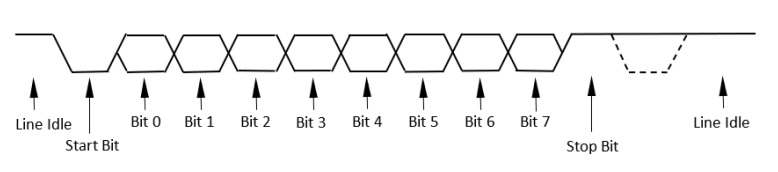
\includegraphics[width=0.8\textwidth]{images/uart_protocol.png}
\caption{Formatul de date UART \cite{uart_poza}}
\label{fig:uart_protocol}
\end{figure}

Pentru realizarea transferului de date este folosit conceptul fundamental al acestui protocol, transmisia bit cu bit secvențială. Datele au un format special, specific, ce include un bit de start ce indică începutul comunicării, în mod configurabil între 5 și 9 biți de date. Un bit de paritate ce este opțional și este folosit în verificare erorilor de transmisie și unul sau doi biți de stop care marchează sfârșitul comunicării și semnalează receptorului că biții au fost transmiși cu succes. O altă caractersitică a transferuli este viteza acestuia (baud rate-ul). Aceasta reprezintă numărul de biți transmiși pe secundă și ia valori comune precum 9600, 38400 și 115200 în funcție de nevoile și performanța sistemului. De menționat este faptul că pe ambele dispozitive se impune folosirea aceleiași viteze de transfer. \cite{pena2020uart}. 

\subsection{I2C}
Protocolul I2C (Inter-Integrated Circuit) este un protocol de comunicație serială sincronă și este utilizat pentru comunicații pe distanțe scurte. Acesta permite ca mai multe dispozitive să fie conectate simultan la o singură magistrală de comunicație și funcționează folosind o arhitectură master-slave. În mod uzual, este folosit pentru a conecta la un microcontroller,  dispozitivele  de tip slave.

\begin{figure}[H]
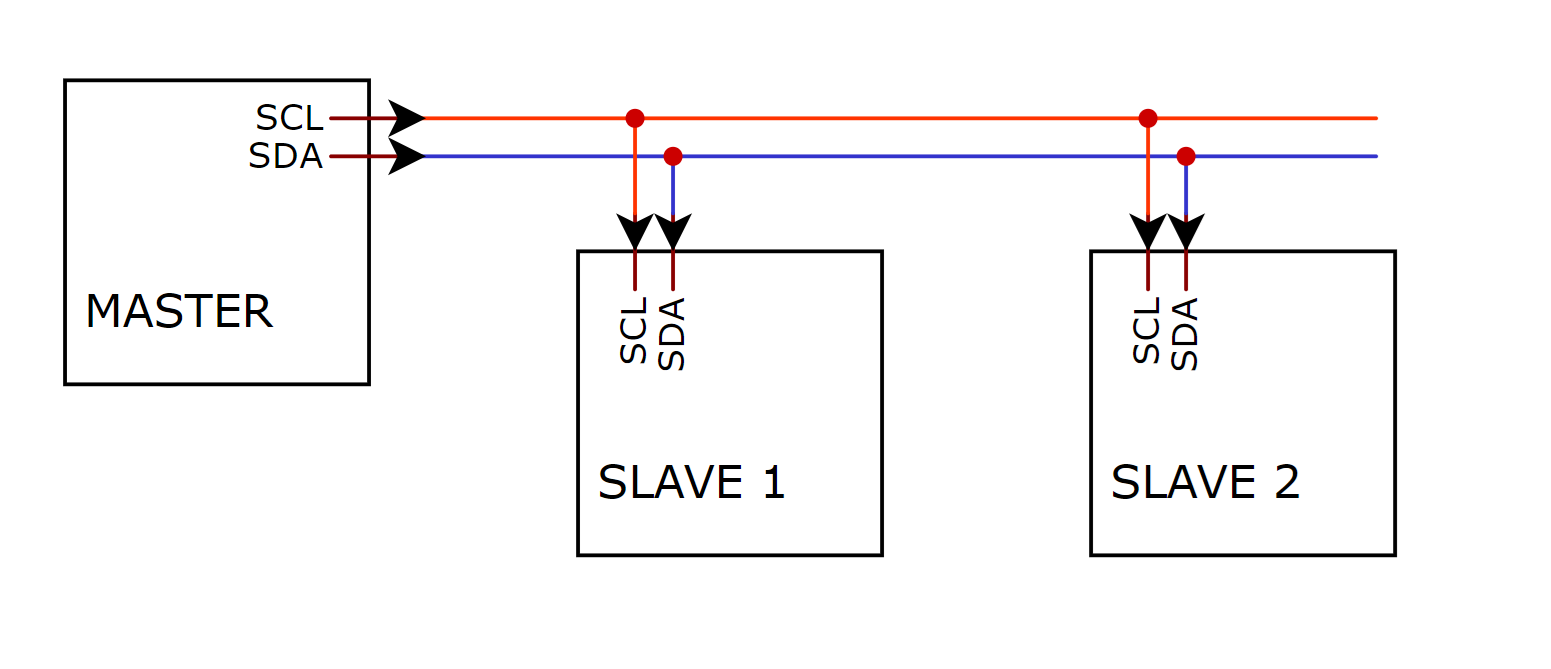
\includegraphics[width=0.7\linewidth]{bachelors_ro/images/i2c_com.png}
\caption{Conectarea dispozitivelor la magistrala I2C}
\label{fig:i2c_com}
\end{figure}

Pentru a realiza comunicarea sunt necesare două linii: SDA (Serial Data Line) și SCL (Serial Clock Line). SCL reprezintă linia de tact ce sincronizează transferul de date, iar SDA linia de date prin care se realizează transferul bidirecțional, dar nu simultan. Master-ul va furniza semnalul de tact. Dispozitivele slave au adrese unice pe magistrala I2C. Astfel, master-ul poate să comunice selectiv cu oricare dintre dispozitivele slave \cite{xu2023design}.

\subsection{Bluetooth}
Bluetooth este un standard de comunicație wireless destinat schimbului de date pe distanțe scurte până în 10 metri. Acesta folosește unde radio la o frecvență de 2.4 GHz. Dispozitivele ce beneficiază de tehnologia Bluetooth se pot conecta la alte dispozitive asemenea atât timp cât respectă raza de comunicare. În timp ce cele două dispozitive sunt conectate, acestea formează o rețea numită piconet. Interconectarea a două sau mai multe rețele piconet duce la formarea unei rețele Scatternet.

În general rata de transfer este cuprinsă între 700 kbps și 3 Mbps pentru versiunile mai vechi, iar pentru versiuni mai noi se poate ajunge până la 25 Mbps. Totodată, transmisia dispune de criptare pentru a preveni interceptarea datelor și de autentificare printr-un cod PIN sau o cheie criptografică \cite{bisdikian2001overview}.

\subsection{WiFi}
WiFi este o tehnologie ce permite conectarea dispozitivelor la internet fără a utiliza cabluri. Principiul de funcționare al WiFi-ului este bazat pe unde radio pentru a transmite date între un punct de acces (sau router) și dispozitivele conectate. Acesta folosește unde radio în banda de frecvență cuprinsă între 2.4 GHz și 5 GHz. Aceste frecvențe sunt folosite pentru a asigura o comunicare eficientă și lipsită de interferențe \cite{chernukhin2014new}.

WiFi utilizează standarde de comunicație precum IEEE 802.11, ce definește modul de transmisie și recepție al datelor. Routerele WiFi folosesc adrese IP pentru a identifica și comunica cu dispozitivele din rețea. DHCP (Dynamic Host Configuration Protocol) este utilizat adesea pentru a atribui în mod automat adrese IP dispozitivelor din rețea. Totodată, WiFi utilizează diverse metode de criptare a datelor transmise, cum ar fi WEP, WPA și WPA2 \cite{hiertz2010ieee}.

\section{Echipamente Hardware}

\subsection{Arduino Mega}
Arduino Mega 2560 R3 este echipată cu microcontrollerul ATmega2560, care oferă o capacitate mare de memorie și mai mulți pini GPIO, făcând-o ideală pentru proiecte avansate ce necesită multiple conexiuni și funcționalități complexe. Placa este compatibilă cu o varietate de shield-uri și module \cite{mega_datasheet}.

\begin{figure}[H]
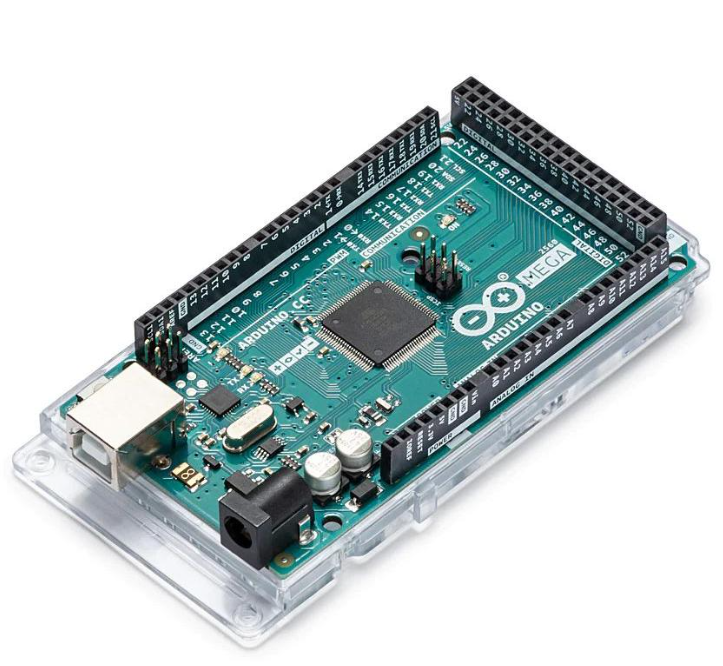
\includegraphics[width=0.7\linewidth]{images/arduino_mega.png}
\caption{Placa de dezvoltare Arduino Mega \cite{mega_poza}}
\label{fig:arduino_mega}
\end{figure}

Specificații tehnice \cite{mega_datasheet}:

\begin{itemize}
  \item Dimensiune placă 101 x 53 mm, greutate 37 g
  \item Tensiunea de alimentare este cuprinsă între 7-12 V
  \item Pini digitali 54, pini analogici 16
  \item Memorie flash de 256 KB din care 8 KB sunt utilizați de bootloader
  \item EEPROM 4 KB
  \item SRAM 8 KB
  \item Frecvența ceas 16 MHz
  \item Oferă și comunicare I2C, USB, SPI, UART
\end{itemize}

\section{Microcontroller-ul ATmega2560}
Microcontroller-ul ATmega2560 dispune de un procesor pe 8 biți din familia AVR, creat de Atmel. AVR este o arhitectură Harvard modificată. Arhitectura este pe 8 biți și este de tip RISC (Reduced Instruction Set Computer). Aceasta este cunoscută pentru eficiența sa energetică și performanța sa când vine vorba de sisteme integrate.

\begin{figure}[H]
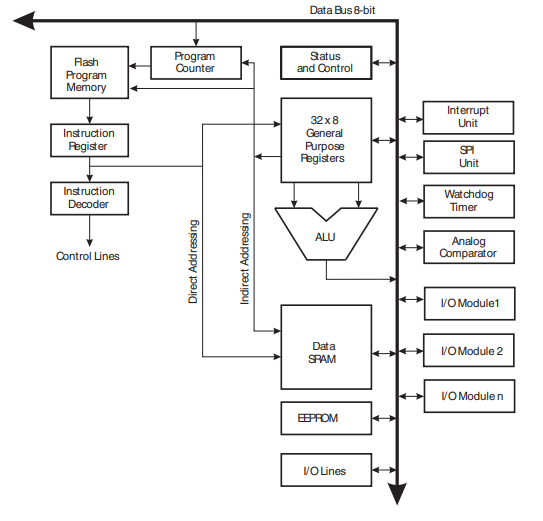
\includegraphics[width=0.6\linewidth]{bachelors_ro/images/arhitectura_avr.png}
\caption{Schema bloc a arhitecturii AVR \cite{avr_atmega2560}}
\label{fig:arhitectura_avr}
\end{figure}

Unitatea centrală de procesare (CPU) AVR este partea cea mai semnificativă a micrcontroller-ului. CPU-ul este comandat de un ceas intern ce funcționează la 16 MHz. Instrucțiunile din memoria de program sunt executate cu ajutorul unui pipeline pe un singur nivel. Astfel, în timp ce o instrucțiune este executată următoare instrucțiune este deja adusă din memoria de program. În Figura \ref{fig:instruction_pipeline} se poate observa cum are loc acest proces. Acestă metodă de bază de pipielining este folosită pentru a obține până la 1 MIPS pe MHz \cite{avr_atmega2560}.

\begin{figure}[H]
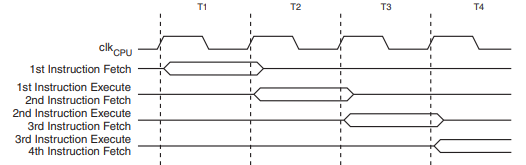
\includegraphics{bachelors_ro/images/instruction_pipeline.png}
\caption{Executarea și aducerea din memorie în paralele executată de procesor \cite{avr_atmega2560}}
\label{fig:instruction_pipeline}
\end{figure}

Această metodă permite ca în fiecare ciclu de tact să fie executată câte o instrucțiune\cite{avr_atmega2560}. Deși mai puțin eficient ca celelalte variante de pipeline, această implementare oferă siguranță împotriva apariției hazardurilor.

\subsection{Modul NodeMCU Lua WIFI ESP8266 CP2102}
NodeMCU ESP8266 este o placă de dezvoltare ce integrează modulul ESP8266, un cip WiFi cu un microcontroler integrat. Aceasta este cunoscută pentru dimensiunile compacte și capacitatea de a oferi o soluție pentru proiectele IoT (Internet of Things). NodeMCU poate fi programat utilizând chiar Arduino IDE și sunt disponibile foarte multe biblioteci pentru acesta\cite{nodemcu_datasheet}.

\begin{figure}[H]
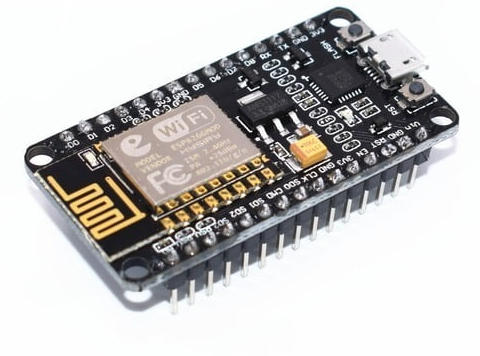
\includegraphics[width=0.5\textwidth, height=0.4\textwidth]{images/nodemcu.png}
\caption{Modul NodeMCU WIFI ESP8266 \cite{nodemcu_poza}}
\label{fig:nodemcu}
\end{figure}

\subsection{Modulul de Bluetooth HC-05}
HC-05 este un modul Bluetooth destinat comunicării seriale fără fir, care permite transferul de date între două dispozitive prin intermediul protocolului Bluetooth. Acesta poate funcționa atât în modurile master, cât și slave, ceea ce înseamnă că poate iniția conexiuni sau poate răspunde la conexiuni inițiate de alte dispozitive. Datele trimise sau primite de acest modul nu necesită nicio decodificare deoarece acestea sunt recepționate bit cu bit.

\begin{figure}[H]
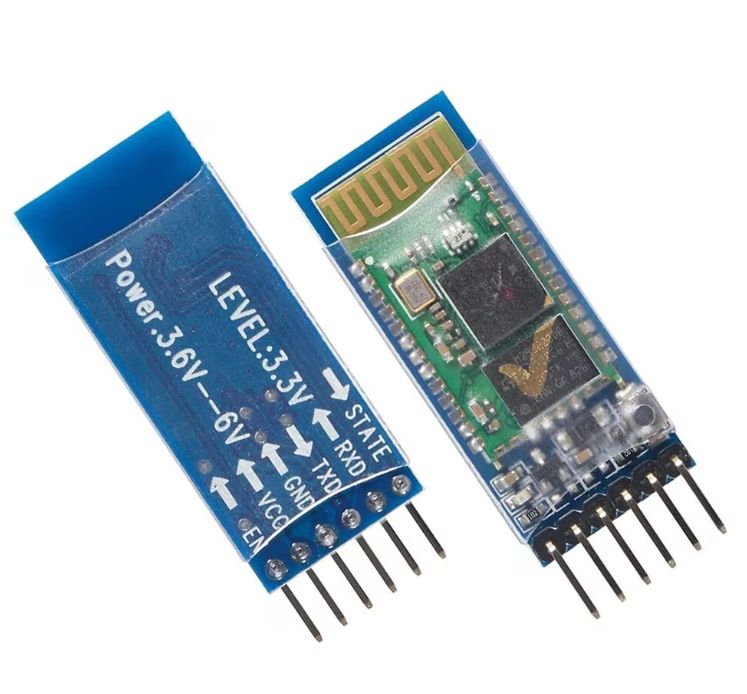
\includegraphics[width=0.3\linewidth]{images/hc05.png}
\caption{Modul Bluetooth HC-05 \cite{hc05_poza}}
\label{fig:hc05}
\end{figure}

\subsection{Display LCD 1602 cu interfață I2C}
Display-ul LCD 1602 cu interfață I2C este un afișaj cu cristale lichide, utilizat popular în proiecte de electronică. Acesta combină un ecran LCD tradițional de 16 caractere pe 2 rânduri cu un modul I2C. Reducând numărul de pini necesari pentru conexiune de la 16 la 4, simplifică integrarea în proiecte. Ținând cont că se folosește de protocolul I2C, acesta se folosește de pinii SDA și SCL pentru a recepționa date.

\begin{figure}[H]
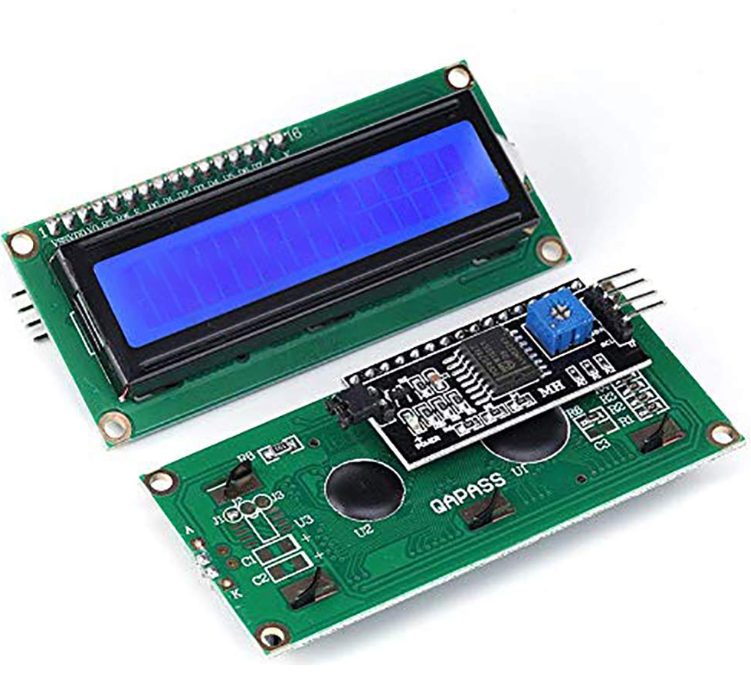
\includegraphics[width=0.4\textwidth, height=0.4\textwidth]{images/lcd.png}
\caption{Display LCD 1602 cu interfață I2C \cite{lcd_poza}}
\label{fig:lcd}
\end{figure}

\subsection{Tastatură 4x4}
Tastatură 4x4 este un keypad matricial care constă din 16 butoane dispuse în formă de matrice. Fiecare buton are o poziție unică, identificată de rândul și coloana sa. Tastatura este de obicei conectată la un microcontroler sau la un alt dispozitiv de control, care citește stările butoanelor pentru a detecta apăsările de taste.

\begin{figure}[H]
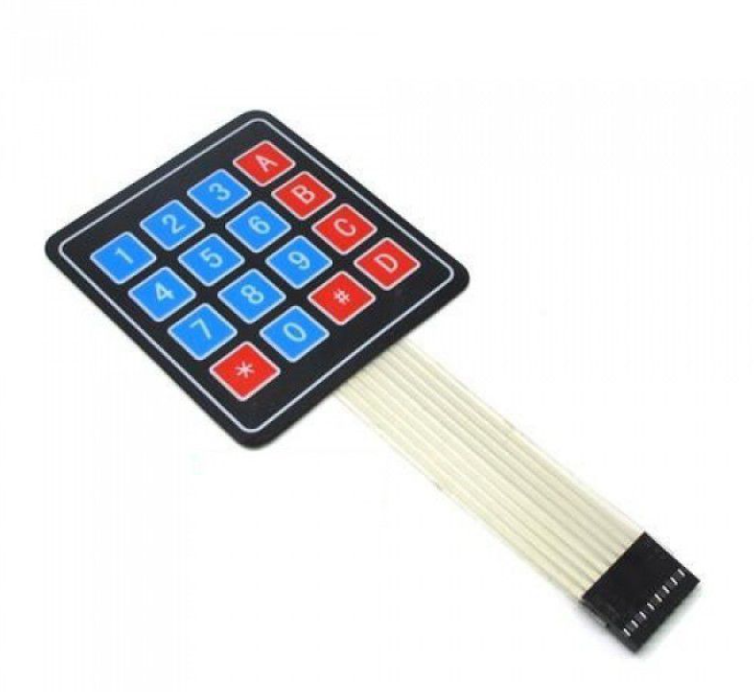
\includegraphics[width=0.4\textwidth, height=0.4\textwidth]{images/tastatura.png}
\caption{Tastatură 4x4 \cite{key_poza}}
\label{fig:tastatura}
\end{figure}


\subsection{Modul Releu}
Un releu este un dispozitiv electric ce funcționează ca un întrerupător, fiind controlat de un circuit electronic. Acesta este utilizat pentru a gestiona circuite de înaltă putere prin intermediul unui semnal de joasă putere. Releul este alcătuit din două componente esențiale: un electromagnet și un set de contacte. Atunci când o tensiune de control este aplicată electromagnetului, se generează un câmp magnetic care acționează asupra unui comutator mecanic, permițând deschiderea sau închiderea circuitului electric.

\begin{figure}[H]
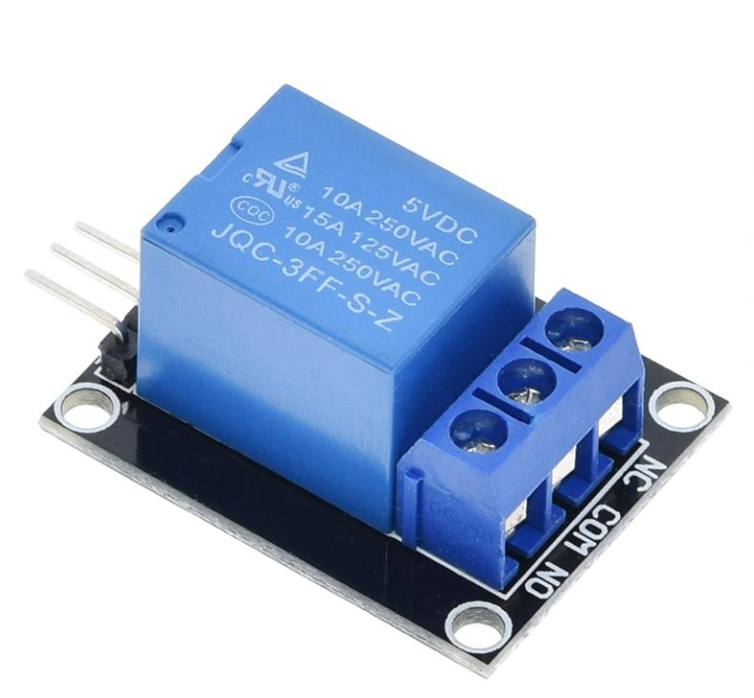
\includegraphics[width=0.3\textwidth, height=0.3\textwidth]{images/releu.png}
\caption{Modul releu cu un singur canal\cite{releu_poza}}
\label{fig:releu}
\end{figure}

\subsection{Senzori}
BMP280 este un senzor de înaltă precizie pentru măsurarea presiunii barometrice și a altitudinii. Fabricat de Bosch Sensortec, acest senzor compact și performant oferă măsurători exacte, fiind perfect pentru aplicații portabile și autonome. Utilizând tehnologia MEMS (Micro-Electro-Mechanical Systems), BMP280 se remarcă prin consumul său redus de energie și fiabilitatea sa în diverse condiții de operare.

\begin{figure}[H]
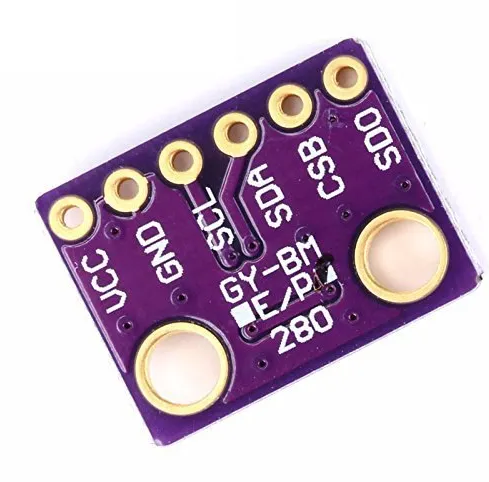
\includegraphics[width=0.3\textwidth, height=0.3\textwidth]{images/bmp.png}
\caption{Senzorul BMP280\cite{bmp_poza}}
\label{fig:bmp}
\end{figure}

DHT11 este un senzor digital folosit pentru a măsura atât temperatura, cât și umiditatea. Datorită ușurinței sale de utilizare este potrivit pentru proiecte de monitorizare a condițiilor de mediu și automatizări casei. Acest senzor integrează un termistor și un senzor capacitiv pentru umiditate, furnizând date precise în format digital.

\begin{figure}[H]
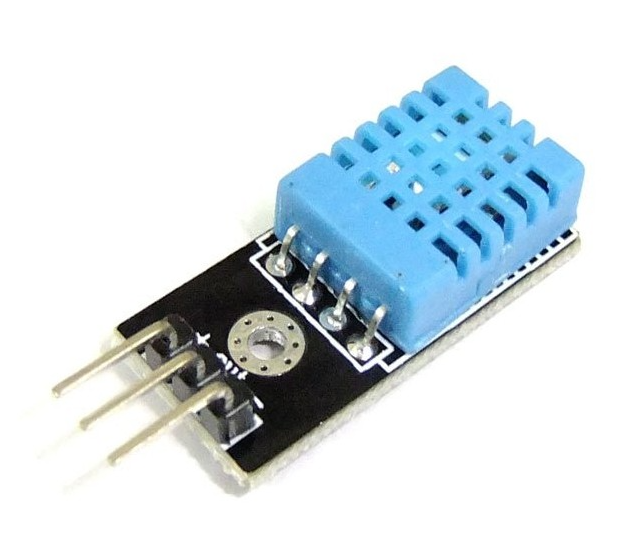
\includegraphics[width=0.3\textwidth, height=0.3\textwidth]{images/dht11.png}
\caption{Senzorul DHT11\cite{dht_poza}}
\label{fig:dht11}
\end{figure}

Senzorul MQ-2 este conceput pentru a detecta concentrații de gaze inflamabile, inclusiv propan, butan, metan și hidrogen, precum și fum. Acest senzor folosește un element sensibil din oxid de staniu (SnO2), care își reduce rezistența electrică în prezența acestor gaze, permițând astfel măsurarea concentrației de gaz.

\begin{figure}[H]
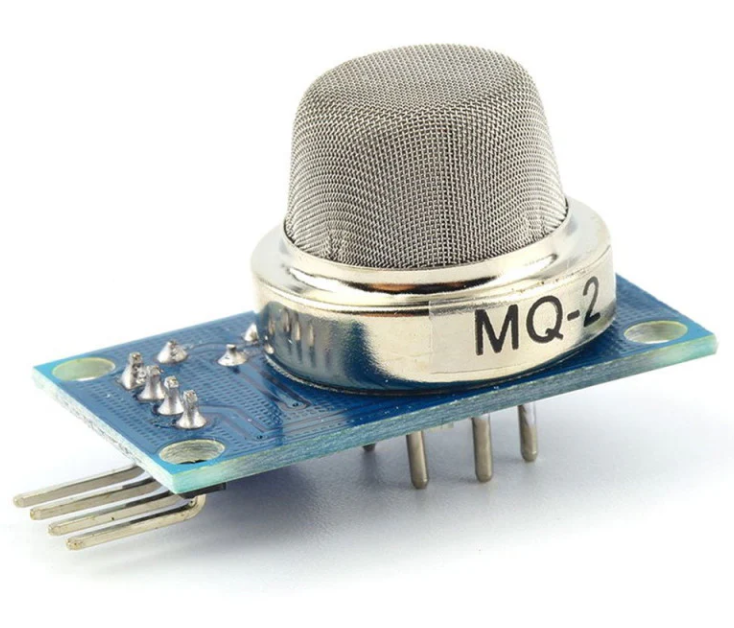
\includegraphics[width=0.3\textwidth, height=0.3\textwidth]{images/mq2.png}
\caption{Senzorul MQ2\cite{mq_poza}}
\label{fig:mq2}
\end{figure}

Un modul cu fotorezistor constă într-un fotorezistor și un circuit de bază, ce include un potențiometru pentru reglarea sensibilității, precum și conexiuni pentru alimentare și transmiterea unui semnal digital . Fotorezistorul, componenta esențială a modulului, își modifică rezistența în funcție de nivelul de lumină la care este expus, permițând astfel generarea unui semnal digital corespunzător.

\begin{figure}[H]
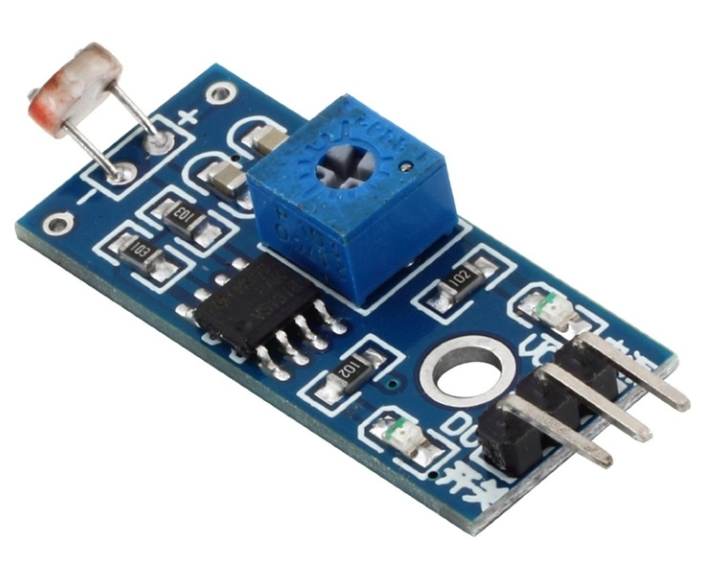
\includegraphics[width=0.3\textwidth, height=0.3\textwidth]{images/senz_lumina.png}
\caption{Modul cu fotorezistor\cite{senzlum_poza}}
\label{fig:senz_lumina}
\end{figure}

HC-SR501 este un senzor PIR (Passive Infrared) care identifică mișcarea detectând modificările în radiația infraroșie din mediul înconjurător. Acesta include un element detector de infraroșu, un circuit de procesare și o lentilă Fresnel, care focalizează radiația infraroșie pe elementul sensibil. Atunci când un obiect cu o temperatură diferită față de fundal (cum ar fi o persoană sau un animal) se deplasează în zona de detectare, senzorul emite un semnal de ieșire.

\begin{figure}[H]
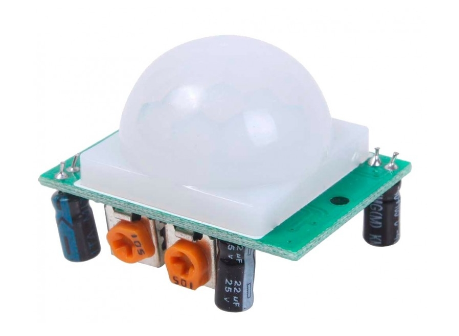
\includegraphics[width=0.4\linewidth]{images/pir.png}
\caption{Senzorul HC-SR501 PIR\cite{pir_poza}}
\label{fig:pir}
\end{figure}

HC-SR04 este un senzor ultrasonic destinat măsurării distanței. Acest senzor funcționează prin emiterea undelor ultrasonice pentru a determina distanța față de un obiect. Are patru pini: VCC, Trig, Echo și GND. Senzorul generează un impuls ultrasonic de 40 kHz prin intermediul pinului Trig și primește ecoul reflectat prin pinul Echo. Intervalul de timp necesar pentru ca semnalul să se reflecte înapoi este utilizat pentru a calcula distanța față de obiectul detectat.

\begin{figure}[H]
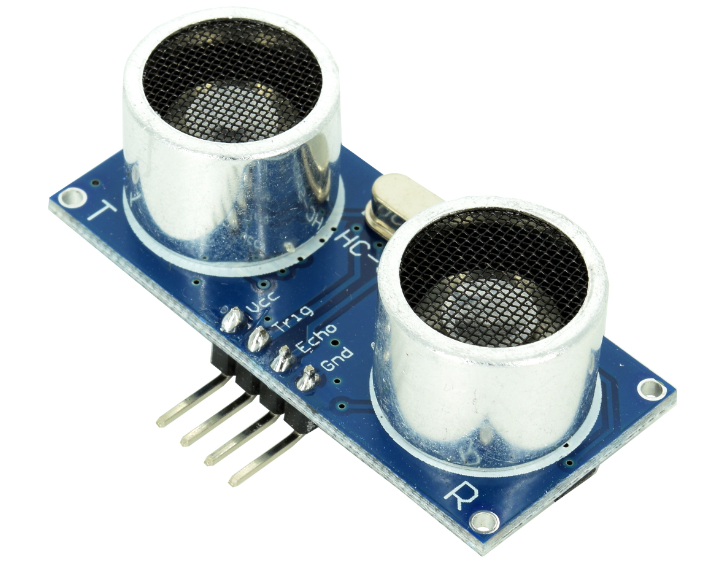
\includegraphics[width=0.4\textwidth, height=0.3\textwidth]{images/ultrasonic.png}
\caption{Senzorul HC-SR04\cite{ultras_poza}}
\label{fig:ultrasonic}
\end{figure}


\subsection{Microservo SG90}
Microservo SG90 este un servomotor compact, care operează utilizând semnale PWM (Pulse Width Modulation). Arborele său de ieșire poate fi reglat la unghiuri cuprinse între 0 și 90 de grade. Acest reglaj se realizează prin modificarea semnalului PWM trimis motorului. Microservo SG90 include un motor DC de mici dimensiuni, un set de angrenaje pentru reducerea vitezei și creșterea cuplului, precum și un circuit de control. Circuitul de control interpretează semnalul PWM de la microcontroller și ajustează poziția arborelui în funcție de durata impulsurilor semnalului.

\begin{figure}[H]
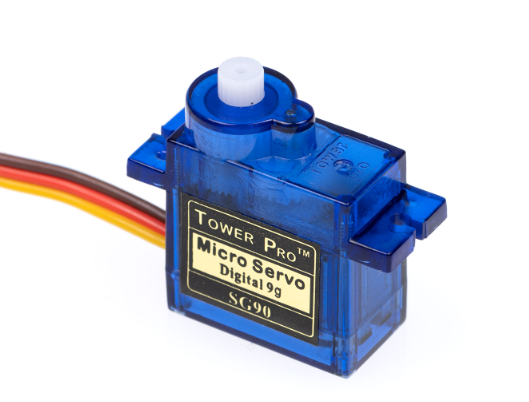
\includegraphics[width=0.4\textwidth, height=0.3\textwidth]{images/servo.png}
\caption{Microservo SG90\cite{servo_poza}}
\label{fig:servo}
\end{figure}

\subsection{Buzzer pasiv și LED}
Buzzerele pasive sunt dispozitive care produc sunet atunci când primesc un semnal cu frecvență variabilă. Acestea transformă semnalul electric în vibrații mecanice, generând astfel unde sonore. Spre deosebire de buzzerele active, cele pasive sunt mai versatile, fiind capabile să emită o varietate de tonuri și sunete în funcție de semnalul de control primit.

\begin{figure}[H]
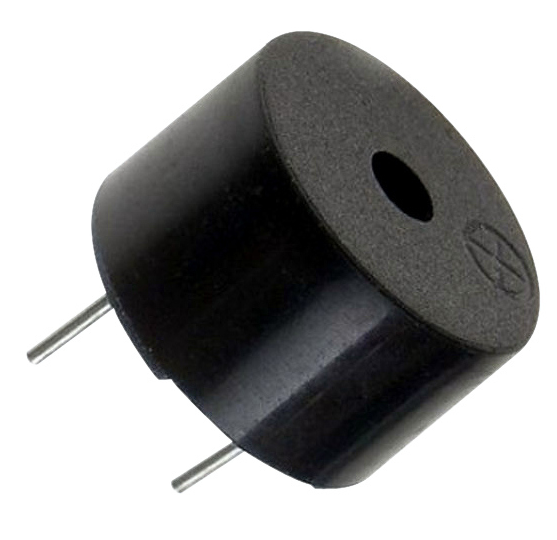
\includegraphics[width=0.3\textwidth, height=0.3\textwidth]{images/buzzer.png}
\caption{Buzzer Pasiv\cite{buzzer_poza}}
\label{fig:buzzer}
\end{figure}

LED-urile sunt diode care emit lumină atunci când un curent electric le parcurge într-o anumită direcție. Acestea sunt disponibile într-o varietate de culori, dimensiuni și forme, fiind utilizate în numeroase aplicații, de la iluminat interior și exterior, până la afișaje digitale, semnalizări și dispozitive electronice. Comparativ cu becurile tradiționale, LED-urile nu au filament și generează foarte puțină căldură, ceea ce le conferă o eficiență energetică superioară.

\begin{figure}[H]
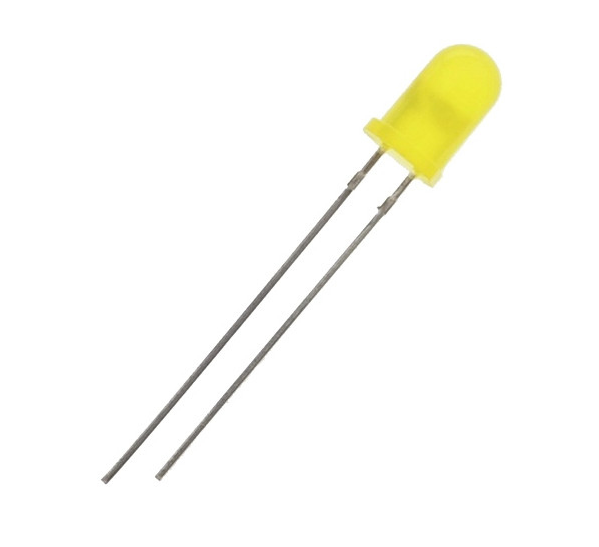
\includegraphics[width=0.3\textwidth, height=0.3\textwidth]{images/led.png}
\caption{LED\cite{led_poza}}
\label{fig:led}
\end{figure}

\subsection{Sursă alimentare 12 V, Ventilator și bec H7}
O sursă de alimentare care convertește tensiunea de 220V AC la 12V DC funcționează prin mai multe etape cheie. În prima fază, curentul alternativ de 220V este transformat în curent continuu pulsatoriu prin intermediul unui circuit redresor, de obicei un pod redresor. Apoi, acest curent continuu pulsatoriu este netezit de un condensator de filtrare, producând un curent continuu mai stabil. Următoarea etapă implică reducerea și stabilizarea tensiunii la 12V folosind un regulator de tensiune sau un convertor DC-DC step-down. De asemenea, sursa de alimentare include circuite de protecție care previn deteriorările cauzate de supratensiuni, scurtcircuite sau supraîncălziri. Toate aceste procese sunt integrate într-un circuit compact, oferind o conversie eficientă și stabilă a tensiunii pentru a asigura funcționarea în siguranță și fiabilitatea dispozitivelor conectate.

\begin{figure}[H]
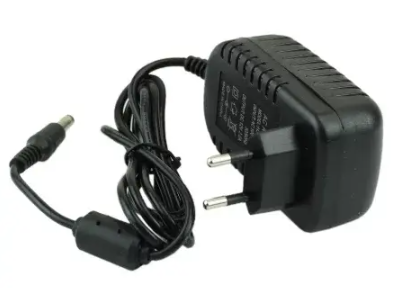
\includegraphics[width=0.4\textwidth, height=0.3\textwidth]{images/sursa.png}
\caption{Sursă de alimentare\cite{sursa_poza}}
\label{fig:sursa}
\end{figure}

Un ventilator funcționează prin convertirea energiei electrice în energie mecanică pentru a produce un flux de aer. Alimentat la o tensiune de 12V DC, motorul electric, adesea de tip brushless, transformă energia electrică în mișcare, rotind axul pe care sunt fixate palele ventilatorului. Această rotație generează un curent de aer, a cărui direcție și intensitate depind de designul și viteza palelelor. Viteza ventilatorului poate fi ajustată manual printr-un controler sau automat, cu ajutorul unui senzor de temperatură.

\begin{figure}[H]
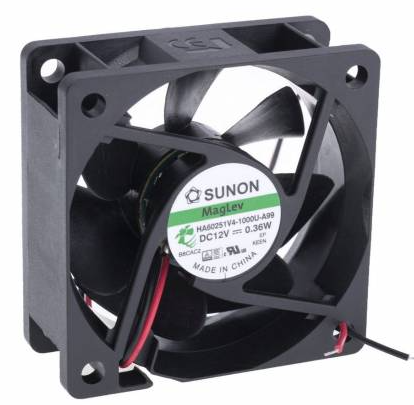
\includegraphics[width=0.3\textwidth, height=0.3\textwidth]{images/ventilator.png}
\caption{Ventilator 12 V\cite{vent_poza}}
\label{fig:ventilator}
\end{figure}

Becul H7 este larg utilizat în sistemele de iluminat auto, fiind recunosccut pentru farurile de fază scurtă și lungă. Acest tip de bec aparține categoriei de becuri halogen și este recunoscut pentru luminozitatea și claritatea luminii pe care o oferă.

Aceste becuri funcționează pe baza principiului halogenului, unde un filament de tungsten este înconjurat de un gaz halogen. Acest design permite becurilor să aibă o durată de viață mai lungă și o temperatură de operare mai mare în comparație cu becurile incandescente tradiționale. Rezultatul este o lumină mai strălucitoare și mai albă, care îmbunătățește vizibilitatea pe timp de noapte și în condiții meteorologice dificile.

\begin{figure}[H]
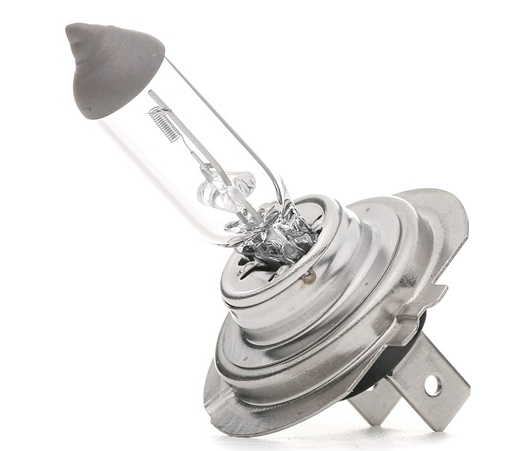
\includegraphics[width=0.3\textwidth, height=0.3\textwidth]{images/bec_h7.png}
\caption{Bec H7\cite{bech7_poza}}
\label{fig:bec_h7}
\end{figure}



\chapter{Fundamente de fiabilitate, redundanţă şi mentenabilitate}
\thispagestyle{pagestyle}
Necesitatea de a menține funcționarea continuă și optimă a sistemelor embedded a condus la dezvoltarea unor principii esențiale pentru implementarea acestor sisteme. Pentru ca un sistem să răspundă cerințelor pentru care a fost creat, nu este suficient să își îndeplinească funcțiile. Acesta trebuie să fie fiabil, să mențină un echilibru adecvat între cost și eficiență și să fie ușor de întreținut.

\section{Fiabilitate}
Fiabilitatea (notată cu R(t)) se referă la abilitatea unui sistem sau a unei componente de a funcționa fără defecțiuni pe o durată de timp specificată (intervalul de timp [$t_0$,t])
 și în condiții de utilizare definite. Aceasta este o trăsătură crucială, deoarece are un impact direct asupra performanței și disponibilității sistemului. Un sistem fiabil reduce la minimum perioadele de nefuncționare și costurile de întreținere, consolidând totodată încrederea utilizatorilor în capacitatea sa de a opera conform specificațiilor stabilite\cite{fiabilitate_curs}, \cite{fault_tolerant}.

 Pentru a asigura un nivel înalt de fiabilitate, este esențial să se efectueze o proiectare minuțioasă, să se utilizeze componente de înaltă calitate și să se desfășoare teste riguroase. Suplimentar, monitorizarea constantă și întreținerea preventivă sunt vitale pentru a menține fiabilitatea pe termen lung. În domeniul sistemelor embedded, fiabilitatea capătă o importanță majoră, deoarece aceste sisteme sunt frecvent implementate în aplicații critice, unde defecțiunile pot avea impacturi semnificative.

 Pentru dispozitivele complexe, respectarea principiului fiabilității implică poziționarea componentelor într-un sistem în două perspective:

\begin{itemize}
\item Din punct de vedere fiabilistic: se subliniază că fiabilitatea unei componente din cadrul sistemului poate influența fiabilitatea altor componente.
\item Din punct de vedere structural: se analizează fiabilitatea sistemului în funcție de aranjarea componentelor.
\end{itemize}


Există patru modalități principale de configurare a componentelor \cite{fault_tolerant}:

\begin{itemize}
\item Serie: Defectarea unei singure componente cauzează defectarea întregului sistem.
\item Paralel: Sistemul continuă să funcționeze până când ultima componentă se defectează; defectarea întregului sistem are loc doar dacă toate componentele se defectează.
\item Serie-paralel: Întregul sistem se defectează numai dacă toate componentele dispuse în paralel se defectează.
\item Paralel-serie: Sistemul se defectează complet dacă toate componentele dispuse în serie se defectează.
\end{itemize}

Luând în considerare aspectele prezentate mai sus, am decis ca în sistemul proiectat de mine să folosesc o dispunere în paralel a componentelor pentru a asigura o fiabilitate cât mai ridicată. O defecțiune la o anumită componentă nu va duce la distrugerea întregului sistem și îi va permite o funcționare parțială, dar totuși relevantă.


\section{Mentenabilitate}


Mentenabilitatea, proprietatea unui sistem de a fi întreținut și reparat cu ușurință, este crucială pentru a asigura funcționarea continuă și eficientă pe termen lung. Aceasta poate fi definită atât calitativ, cât și cantitativ. Din perspectivă calitativă, mentenabilitatea se referă la capacitatea unui sistem de a funcționa fără defecțiuni într-o anumită perioadă de timp. Din punct de vedere cantitativ, aceasta reprezintă capacitatea sistemului de a îndeplini funcțiile pentru care a fost implementat \cite{fault_tolerant}.

Mentenabilitatea include atât întreținerea preventivă, care are ca scop evitarea defecțiunilor prin inspecții și ajustări regulate, cât și întreținerea corectivă, concentrată pe repararea sau înlocuirea componentelor defecte după apariția unei probleme. Este esențială în proiectarea sistemelor, influențând direct costurile de operare și timpul de nefuncționare.

Un sistem cu o mentenabilitate ridicată permite tehnicienilor să identifice rapid problemele, să acceseze cu ușurință componentele necesare pentru reparații și să finalizeze lucrările necesare într-un interval de timp scurt. Proprietatea de mentenabilitate devine foarte importantă în perioada de maturitate a produsului, după ce acesta a fost introdus pe piață și pus în funcțiune, deoarece este principalul factor care trebuie luat în calcul pentru a menține performanțele sistemului și pentru a minimiza costurile și timpul de nefuncționare.

Astfel, în sistemul creat de mine componentele pot fi înlocuite individual, fără a fi nevoie ca întreg sistemul să fie dezasamblat. Atât timp cât dispunem de componente noi pentru înlocuirea celor defectate, timpul de nefuncționare ar trebui să fie de ordinul minutelor.

\section{Redundanţă}
Redundanța implică adăugarea de componente suplimentare sau sisteme alternative într-un design pentru a îmbunătăți fiabilitatea și disponibilitatea acestuia. Atunci când apare o defecțiune, aceste elemente redundante preiau funcțiile componentelor defecte, garantând continuitatea operării sistemului \cite{fault_tolerant}.

Putem avea 4 modalități de implementare a redundanței:

\begin{itemize}
\item Hardware
\item Software
\item Informațional
\item Temporal
\end{itemize}

Redundanța hardware constă în folosirea unor echipamente suplimentare, cum ar fi surse de alimentare, procesoare sau unități de stocare duplicate. Redundanța software presupune implementarea unor algoritmi sau programe alternative capabile să preia controlul în cazul unei erori a software-ului principal. Redundanța informațională implică replicarea și distribuirea datelor pe multiple suporturi sau locații pentru a preveni pierderea acestora. Redundanța temporală se referă la executarea unor operații sau procese critice în momente diferite, asigurând astfel, că în cazul unui eșec inițial, există posibilitatea reîncercării fără a compromite funcționarea generală a sistemului.

În sistemul creat de mine am implementat atât redundanță hardware, cât și informațională. Redundanța hardware provine din faptul că datele adunate de senzori sunt transmise atât prin Bluetooth către aplicația mobilă creată de mine, prin WiFi către Cloud-ul Blynk unde se pot urmări folosind aplicația web sau mobile oferită de aceștia și nu în ultimul rând pe LCD-ul atașat sistemului. Astfel, dacă una sau două dintre căile de vizualizare a datelor se defectează încă este posibil ca sistemul să fie supravegheat. Redundanța informațională este oferită cu ajutorul Cloud-ului Blynk, unde informațiile înregistrate până la momentul defectării sau al statusului de offline, sunt înregistrate și pot fi exportate.

\section{Fault Tree Analysis}
Fault Tree Analysis (FTA) este o metodă deductivă utilizată pentru a identifica și evalua cauzele potențiale ale defecțiunilor în sistemele complexe. Această tehnică ajută la determinarea modului în care diverse defecțiuni ale componentelor pot duce la o defecțiune generală a sistemului. Aceste defecțiuni neplăcute pot fi cauzate de probleme software, hardware sau de erori umane \cite{fiabilitate_curs}.

Metoda deductivă începe cu o concluzie generală și se focalizează pe identificarea cauzelor specifice până la cel mai detaliat element care poate contribui la acea concluzie. Prin acest proces, se construiește un arbore al defecțiunilor provenite din cauze multiple sau simple.

Scopul principal al analizei acestui arbore este de a ajuta la identificarea cauzelor potențiale de defectare a sistemului înainte ca acestea să se producă efectiv.

Pentru a detecta cauzele defecțiunii este folosit arborele din Figura \ref{fig:fta}. Modul de parcurgere al acestuia este de sus în jos și este interpretat pe nivele. Evenimentul principal este \texttt{System failure} (Defectarea sistemului) și folosind poarta \texttt{OR}, acestă defecțiune poate apărea din două motive: \texttt{sensor failure} (defecțiunea senzorilor) sau \texttt{Control boards failure} (defecțiunea plăcilor de control). La rândul lor, aceste două defecțiuni pot apărea din varii motive. Defecțiunea senzorilor poate apărea dintr-o lipsă de alimentare sau dintr-o interpretare incorectă a datelor. Defecțiunea plăcilor de control poate fi determinată de o eroare software în codul rulat sau de o eroare de hardware care poate apărea la rândul ei din alte două motive: lipsa alimentării sau o eroare a microcontroler-ului.

\begin{figure}[H]
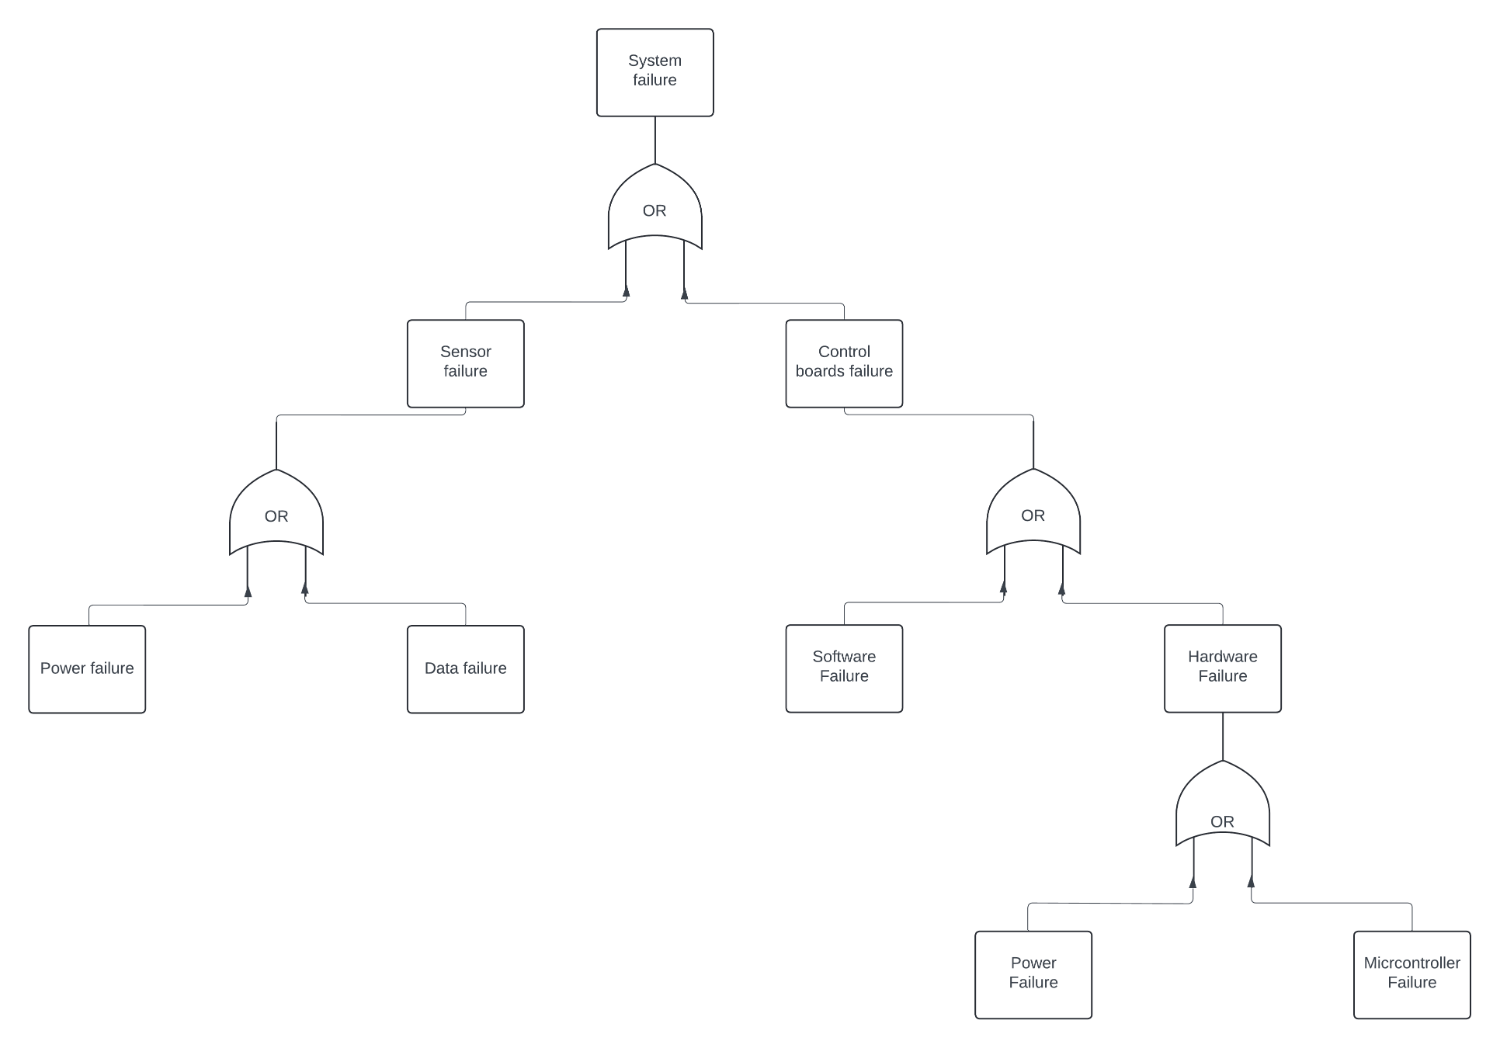
\includegraphics[width=1\linewidth]{images/fta.png}
\caption{Fault Tree Analysis pentru sistemul implementat}
\label{fig:fta}
\end{figure}


\chapter{Arhitectura Hardware}
\thispagestyle{pagestyle}
\section{Schema hardware bloc a sistemului}

\begin{figure}[h]
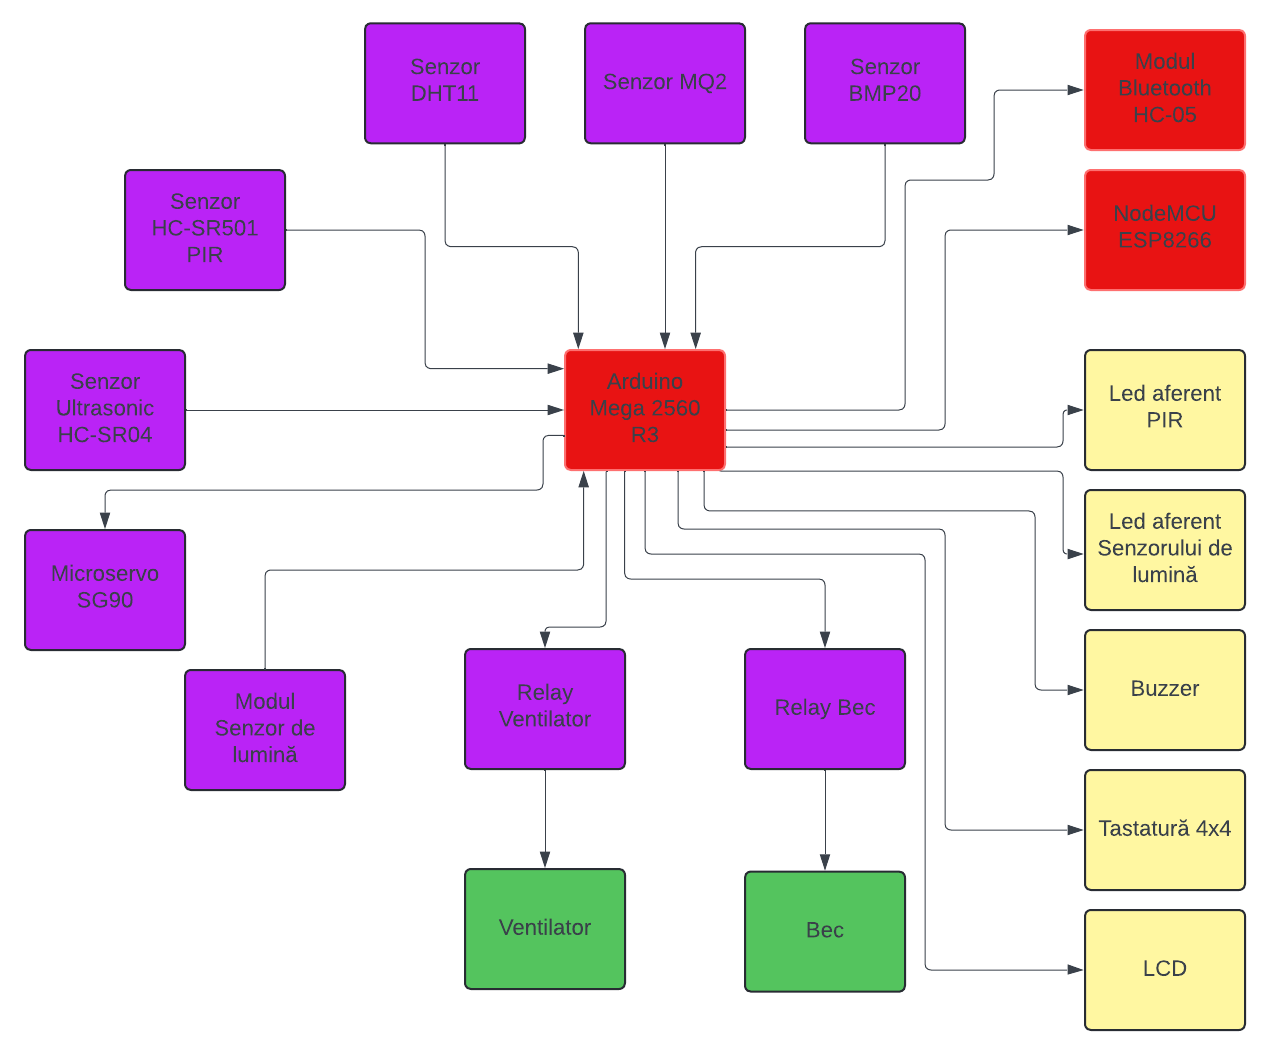
\includegraphics[width=1\textwidth]{bachelors_ro/images/schema_bloc.png}
\caption{Schema hardware bloc a sistemului}
\label{fig:schema_bloc}
\end{figure}

În figura \ref{fig:schema_bloc} este prezentată schema bloc a sistemului modelat de mine. Scopul acestei arhitecturi este de a controla componente precum led-urile, servomotorul și buzzer-ul cu ajutorul datelor oferite de senzori. Astfel, componentele din chenarele mov reprezintă componentele ce oferă diverse date (senzori), iar cel verzi și galbene reprezintă componentele ce execută diverse funcții conform necesităților aferente. În chenarele roșii sunt componentele ce primesc informații interpretate de placa de dezvoltare Arduino Mega și le trimit mai departe prin intermediul WiFi-ului către Cloud-ul Blynk și prin Bluetooth către aplicația Andorid.

Majoritatea senzorilor sunt legați folosind fire la pinii digitali ai plăcii, cu excepția senzorului MQ2 ce este conectat la un pin analogic și senzor BMP280 ce folosește protocolul I2C. Legătura dintre Arduino Mega cu Modulul Bluetooth, respectiv NodeMCU ESP8266, se face prin interfețele seriale UART oferite de placă.

\section{Realizarea montajului arhitecturii Hardware}
Pentru a realiza montajul afarent arhitecutrii implementate am ales să folosesc o placă dedicată PCB (Printed Circuit Board). Astfel, am lipit direct pe aceasta placa de dezvoltare Arduino Mega, NodeMCU ESP8266 și modul de Bluetooth HC-05 cu ajutorul cositorului și a gărdulețelor de pini. Pentru modulul Bluetooth și NodeMCU am folosit jumpere pentru a putea întrerupe comunicarea serială între acestea și Arduino Mega, deoarce aceasta trebuie să fie oprită dacă doresc să urc cod nou pe placa Arduino Mega, dar și pe NodeMCU. 

Pentru restul componentelor am folosit fire de diverse culori și grosimi pentru a fi mai ușor identificabile. Aceste cabluri au lipite direct de pinii plăcii Arduino cu cositor, iar la capete au fost modificate fie cu mufe mama, fie cu mufe tată în funcție de nevoie. În Figura \ref{fig:sechema_full_sistem} este prezentată schema de conectare a întregului sistem.

\begin{figure}[H]
    \centering
    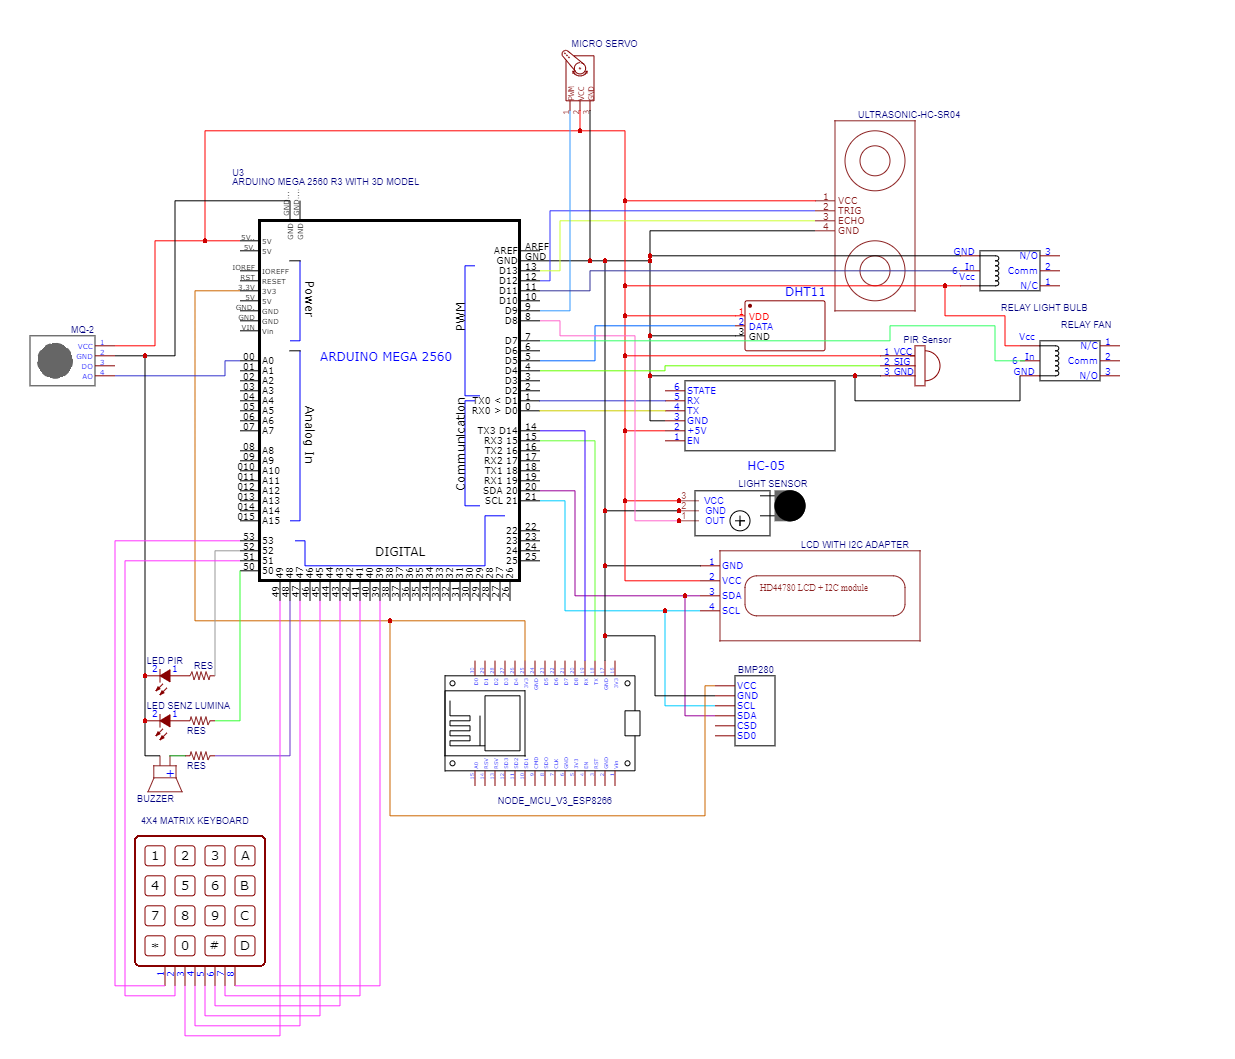
\includegraphics[width=1\linewidth]{bachelors_ro/images/sechema_full_sistem.png}
    \caption{Schema de conectare a sistemuui}
    \label{fig:sechema_full_sistem}
\end{figure}
\chapter{Implementarea Hardware}
\thispagestyle{pagestyle}

Pentru implementarea hardware am decis să aleg o placă de dezvoltare oferită de Arduino cu performanțe superioare din toate aspectele necesare dezvoltării, și anume Arduino Mega 2560 Rev3. Cu un microcontroler performant aceasta îndeplinește toate criteriile necesare pentru realizarea sistemului. Placa de dezvoltare dispune de 54 de pini digitali, incluzând și toate funcțiile suplimentare de care aveam nevoie: 15 pini ce dispun de PWM, 4 cupluri de pini pentru comunicare serială și pinii pentru comunicarea prin protocolul I2C\cite{mega_datasheet}.

Astfel, cu placa de dezvoltare aleasă și cu arhitectura gândită a început procesul de implementare hardware al componentelor.

\section{Conectarea modulului NodeMCU Lua WIFI ESP8266 CP2102}
Primul pas a fost realizarea comunicării seriale dintre Arduino Mega și modulul NodeMcu pentru a avea acces la WiFi. Modulul trebuie alimentat la 3.3 V fapt ce a fost facilitat de faptul că Arduino Mega dispune de un pin ce oferă o tensiune de 3.3 V fără a mai fi nevoie de un stabilizator de tensiune auxiliar. Apoi, am conectat pinul de GND al plăcii cu cel al modului. Ultimul pas a fost să leg pinii ce realizează comunicarea serială. Am ales a treia interfață serială disponibilă pe Arduino Mega și am conectat pinii dedicați RX (pinul D15) și TX (pinul D14) ai plăcii la pinii dedicați ai modulului RX și TX.
\begin{figure}[H]
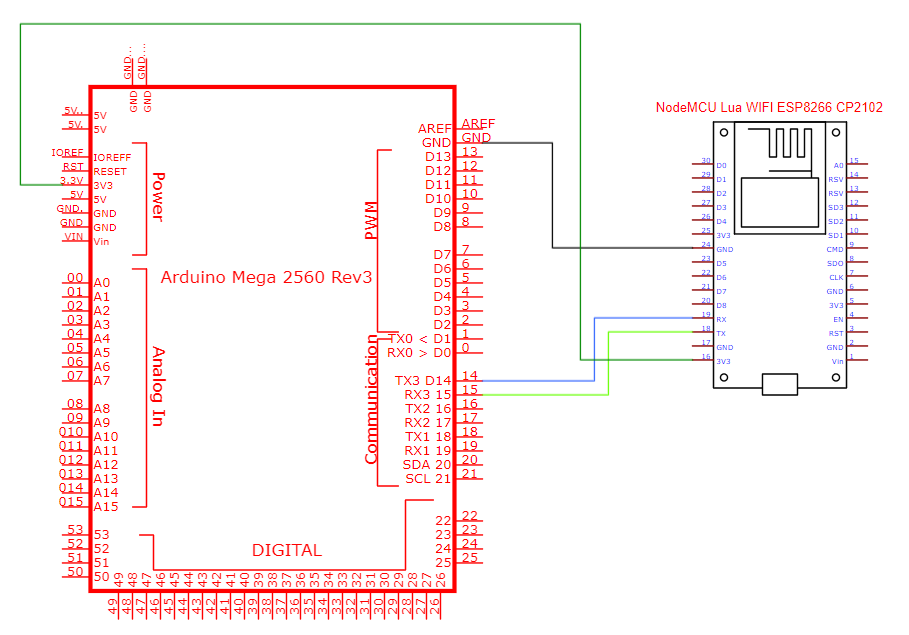
\includegraphics[width=0.9\linewidth]{bachelors_ro/images/conexiune_mega_esp.png}
\caption{Schema de conectare Arduino Mega - NodeMCU}
\label{fig:conexiune_mega_esp}
\end{figure}

\section{Conectarea modulului HC-05}
Următorul pas a fost să realizez comunicarea serială dintre placă și modulul de Bluetooth HC-05. Cele două comunică serial, apoi modulul trimite prin Bluetooth datele mai departe. HC-05 are 6 pini: STATE, RX, TX, GND, 5V, EN. Dintre aceștia a fost nevoie doar de 4. Astfel, pinul de 5V a fost conectat la pinul de alimentare de 5V disponibil pe placa, pinii RX și TX la cuplul RX0 și TX0 al plăcii, iar GND la GND plăcii.

\begin{figure}[H]
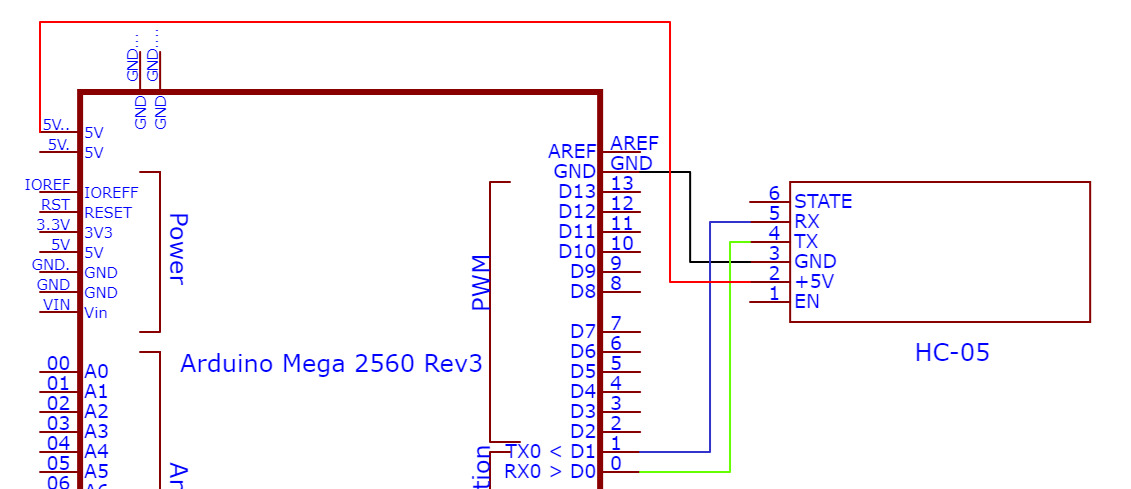
\includegraphics[width=0.7\textwidth, height=0.3\textwidth]{bachelors_ro/images/conexiune_mega_hc05.png}
\caption{Schema de conectare Arduino Mega - HC-05}
\label{fig:conexiune_mega_hc05}
\end{figure}

\section{Conectarea ansamblului de stabilizare a temperaturii}
Montajul ansamblului de stabilizare a temperaturii este format dintr-un senzor de temperatura și umiditate DHT11, un ventilator, un bec H7. Becul și ventilatorul au nevoie de o alimentare de 12 V. Astfel, am ales să folosesc o sursă externă de 12V ce alimentează componentele menționate. Declanșatoarele pentru acestea sunt reprezentate de două relee, ce comută în funcție de o temperatură de prag presetată. În cazul în care temperatura este mai mică decât cea de prag se activează becul, iar dacă este mai mare se activează ventilatorul. 

În Tabelul \ref{tab:conexiune_mega_relee} este prezentată modalitatea în care au fost legați pinii plăcii de cele două relee.
\begin{table}[H]
\caption{Legăturile dintre Arduino Mega și cele doua relee de control}
\label{tab:conexiune_mega_relee}
\begin{tabular}{|l|c|c|c|c|}
\hline
Arduino Mega     & D7 & D11 & 5V & GND \\ \hline
Releu ventilator & S  &     & +  & -   \\ \hline
Releu bec        &    & S   & +  & -   \\ \hline
\end{tabular}
\end{table}

Firul de alimentare de la sursa externă a fost introdus în releu la contactul COM (Common), iar din releu a fost tras un fir de la contactul NC (Normally Closed) la alimentarea ventilatorului. Firul de ground al sursei a fost dus direct la groundul ventilatorului. În aceeași manieră s-a procedat și în cazul becului.
\begin{figure}[H]
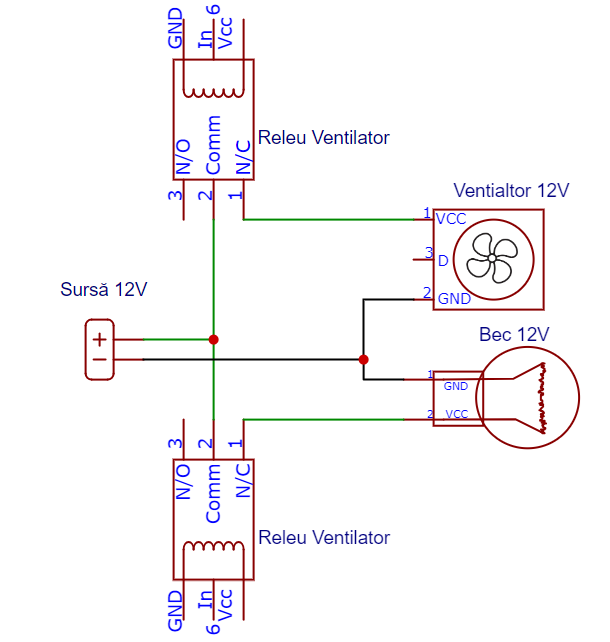
\includegraphics[width=0.6\textwidth, height=0.6\textwidth]{bachelors_ro/images/conexiune_relee_bec_vent.png}
\caption{Schema de conectare Sursă 12V - Relee - Bec/Ventilator}
\label{fig:conexiune_relee_bec_vent}
\end{figure}

Senzorul de umiditate și temperatură DHT11 are 3 pini: S, +, -. Aceștia sunt conectați astfel la placa de dezvoltare.

\begin{table}[H]
\caption{Legăturile dintre Arduino Mega și senzorul DHT11}
\label{tab:conexiune_mega_dht11}
\begin{tabular}{|l|c|c|c|}
\hline
Arduino Mega & D5 & 5V & GND \\ \hline
DHT11 & S & + & - \\ \hline
\end{tabular}
\end{table}

Conform Tabelului \ref{tab:conexiune_mega_relee},\ref{tab:conexiune_mega_dht11} și Figurii \ref{fig:conexiune_relee_bec_vent} ansamblul rezultat este reprezentat în Figura \ref{fig:conexiune_ansamblu_temp}.

\begin{figure}[H]
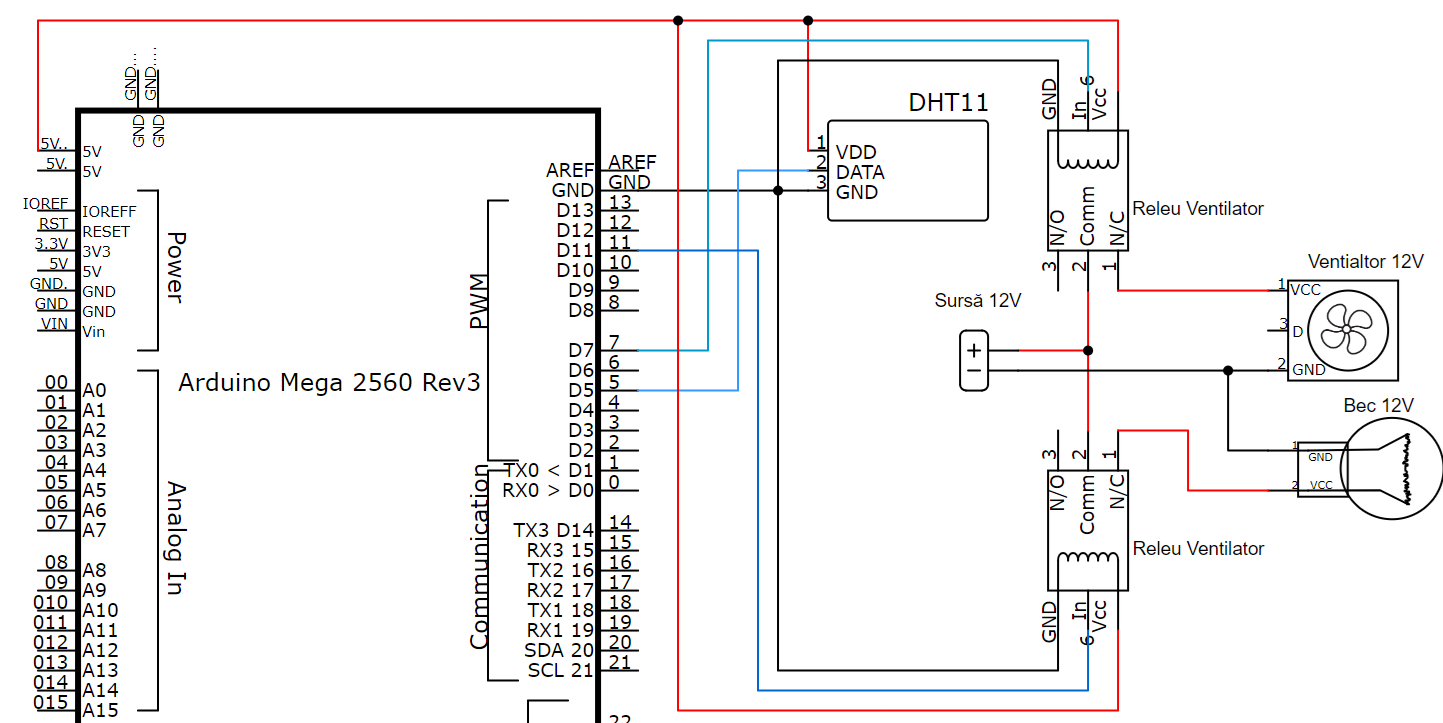
\includegraphics[width=1\linewidth]{bachelors_ro/images/conexiune_ansamblu_temp.png}
\caption{Schema de conectare a ansamblului de stabilizare a temperaturii}
\label{fig:conexiune_ansamblu_temp}
\end{figure}

Ultima componentă pentru a seta temperatura de prag este o tastatură de 4 rânduri și 4 coloane ce permite introducerea acesteia. Tastatura se leagă la 8 pini digitali, 4 pini pentru rânduri și 4 pentru coloane. Legăturile se realizează conform Tabelului \ref{tab:conexiune_tastaura}

\begin{table}[H]
\caption{Legăturile dintre Arduino Mega și Tastatura 4x4}
\label{tab:conexiune_tastaura}
\begin{tabular}{|l|c|c|l|c|l|l|l|l|}
\hline
Arduino Mega & D53 & D51 & D49 & D47 & D45 & D43 & D41 & D39 \\ \hline
Tastatură 4x4 & ROW1 & ROW2 & ROW3 & ROW4 & COL1 & COL2 & COL3 & COL4 \\ \hline
\end{tabular}
\end{table}

Astfel, în Figura \ref{fig:conexiune_tastatura} este prezentat modul de legătură dintre tastatura 4x4 și Arduino Mega.

\begin{figure}[H]
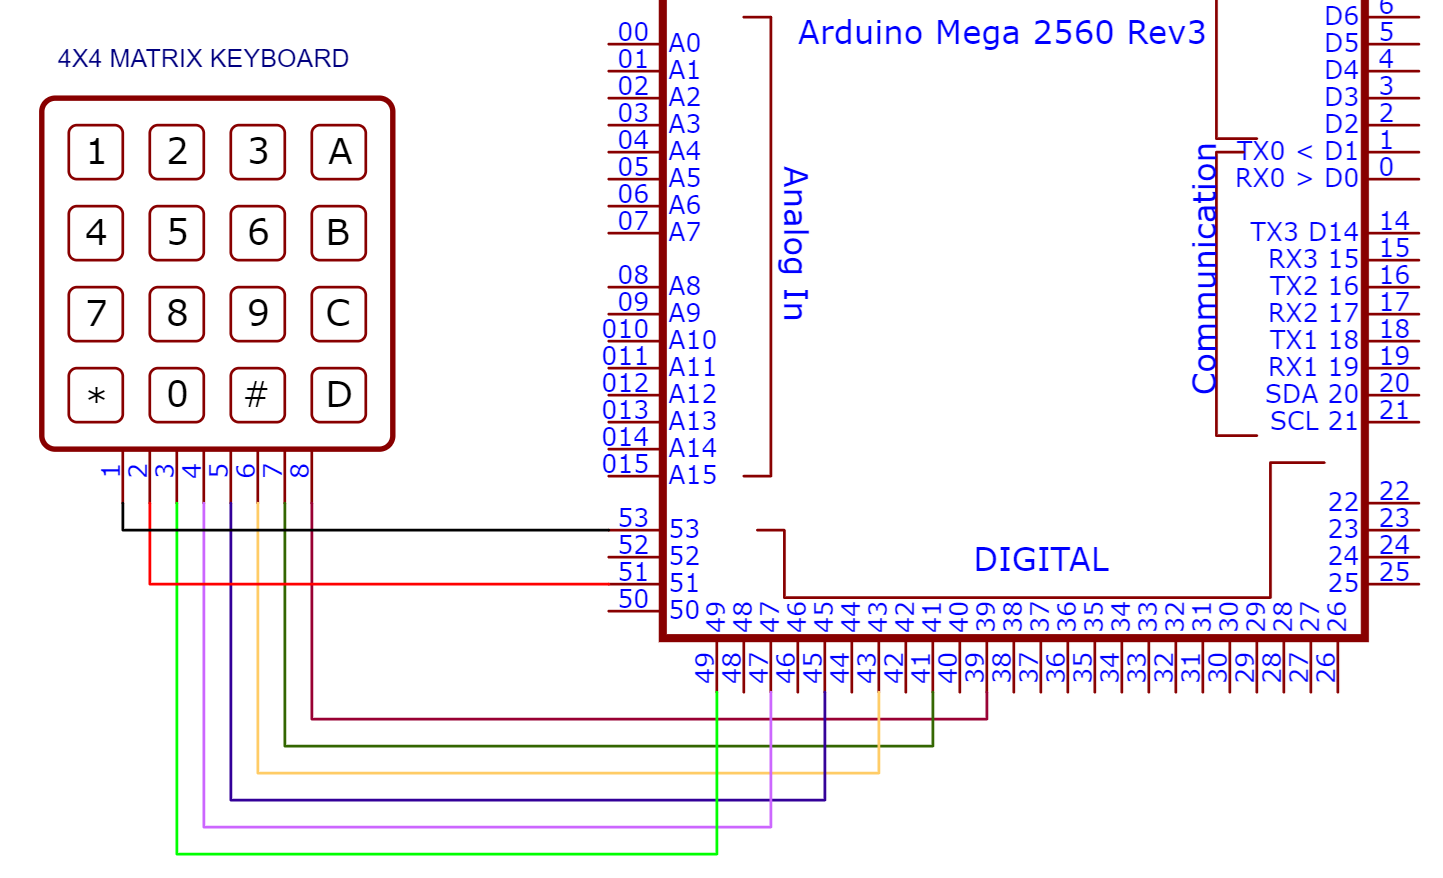
\includegraphics[width=0.5\linewidth]{bachelors_ro/images/conexiune_tastatura.png}
\caption{Schema de conectare dintre tastatură și Arduino Mega}
\label{fig:conexiune_tastatura}
\end{figure}

\section{Conectarea Senzorului de presiune barometrică și a display-ului LCD cu ajutorul protocolului I2C}
Atât senzorul de presiune barometrică BMP280, cât și display-ul LCD 1602 comunică cu placa Arduino Mega prin intermediul protocolului I2C.

În mod tradițional LCD-ul comunică prin mai mulți pini digitali cu placa de dezvoltare, însă celui folosit în proiect i-a fost adăugat o interfață ce permite comunicarea acestuia cu Arduino Mega utilizând protocolul I2C. Astfel, numărul de pini folosiți pentru comunicare a fost redus de la 16 la doar 4 pini specifici modulelor ce folosesc I2C: VCC, GND, SDA (Serial Data Line) și SCL (Serial Clock Line). Echivalent, senzorul de presiune barometrică dispune de exact aceiași pini.

Senzorul de presiune barometrică BMP280 dispune de 6 pini: VCC, GND, SDA, SCL, CSD, SD0. Pentru realizarea montajului s-au folosit doar 4 dintre aceștia (VCC, GND, SCL, SDA). Totodată, senzorul are nevoie de o tensiune de alimentare de 3.3 V spre deosebire de LCD, acesta având nevoie de 5 V. Astfel, firul de alimentare nu poate fi comun pentru cele două.

În Tabelul \ref{tab:conexiune_mega_lcd_bmp} este prezentat modul în care trebuie conectate componentele la Arduino Mega utilizând pinii D20 (SDA) și D21 (SCL) dedicați comunicării I2C.

\begin{table}[H]
\caption{Legăturile dintre Arduino Mega și \\componentele ce comunică prin I2C}
\label{tab:conexiune_mega_lcd_bmp}
\begin{tabular}{|l|c|c|c|l|c|}
\hline
Arduino Mega & D20 & D21 & 5V & 3.3V & GND \\ \hline
LCD 1602 & SDA & SCL & VCC & & GND \\ \hline
BMP280 & SDA & SCL & & VCC & GND \\ \hline
\end{tabular}
\end{table}

Ținând cont de faptul că ambele componente folosesc protocolul I2C pentru a comunica cu microcontroler-ul, fiecare are o adresă unică prezentată în Tabelul \ref{tab:adres_i2c}. Master-ul în acesta caz este reprezentat de microcontroler, iar componentele sunt elementele slave. Pentru a comunica, master-ul inițializează comunicarea folosind o condiție de start, apoi trimite adresa dispozitivului cu care dorește să comunice. Astfel, schimbul de date se face folosind linia SDA (Serial data line) și este sincronizat de SCL (Serial clock line). Pentru încheierea transferului, master-ul generează o condiție de stop. 

\begin{table}[H]
\caption{Adresele componentelor de pe magistrala I2C}
\label{tab:adres_i2c}
\begin{tabular}{|l|c|}
\hline
\textbf{Componenta} & \textbf{Adresa} \\ \hline
BMP280              & 0x76            \\ \hline
LCD 1602            & 0x27            \\ \hline
\end{tabular}
\end{table}

Pentru a realiza conexiunile a fost necesară separarea firelor SDA și SCL în două deoarece se pot folosi doar pinii D20 (SDA) și D21 (SCL) pentru a se realiza comunicarea. Astfel, în Figura \ref{fig:conexiune_bmp_lcd} este prezentată realizarea montajului celor două componente.

\begin{figure}[H]
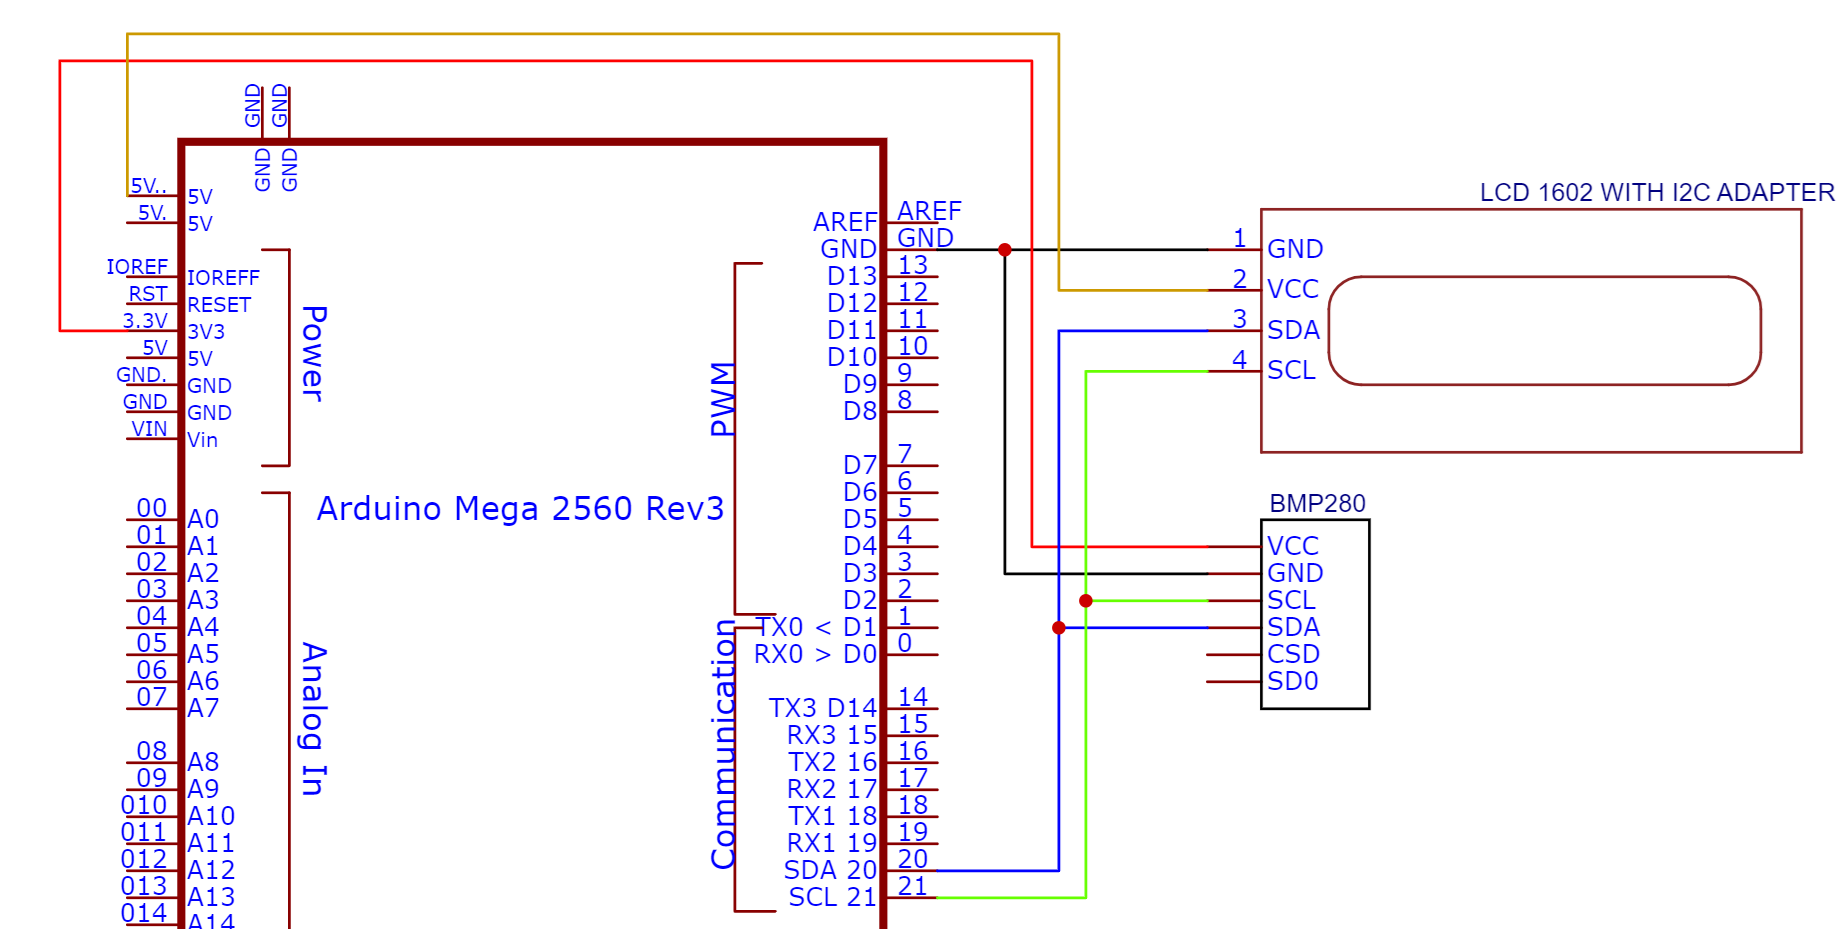
\includegraphics[width=1\textwidth, height=0.5\textwidth]{bachelors_ro/images/conexiune_bmp_lcd.png}
\caption{Schema de conectare a senzorulu de presiune barometrică și a LCD-ului}
\label{fig:conexiune_bmp_lcd}
\end{figure}

\section{Conectarea ansamblului de deschidere automată a ușii}
Ansamblul de deschidere automată a ușii este format din senzorul ultrasonic HC-SR04 și servomotorul SG90. La detectarea mișcării la o anumită distanță predefinită, senzorul trimite un semnal ce activează modificarea poziției servomotorului de la 0 la 180 de grade, astfel deschizând ușa. Apoi, după câteva secunde revine la poziția inițială.

Ambele componente au nevoie de un fir de alimentare comun legat la pinul de 5 V al plăcii și de un GND comun legat la pinul de GND al plăcii. Senzorul ultrasonic trimite date prin pinii ECHO și TRIG către doi pini digitali de pe Arduino Mega, iar servomotorul este controlat folosind un pin digital ce dispune de PWM(Pulse Width Modulation) de pe placă ce este legat la pinul D0 al servomotorului. Astfel, în Tabelul \ref{tab:conexiune_mega_hcsr04_servo} sunt prezentați pinii aleși pentru cele două componente.

\begin{table}[H]
\caption{Legăturile dintre Arduino Mega, Servomotor și Senzorul Ultrasonic}
\label{tab:conexiune_mega_hcsr04_servo}
\begin{tabular}{|l|c|c|c|l|c|}
\hline
Arduino Mega & D9(PWM) & D12 & D13 & 5 V & GND \\ \hline
Servomotor SG90 & D0 & & & VCC & GND \\ \hline
Senzorul HC-SR04 & & TRIG & ECHO & VCC & GND \\ \hline
\end{tabular}

\end{table}

În Figura \ref{fig:conexiune_servo_hcsr04} este prezentat montajul ansamblului format din Arduino Mega, Senzorul Ultrasonic HC-SR04 și servomotorul SG90.

\begin{figure}[H]
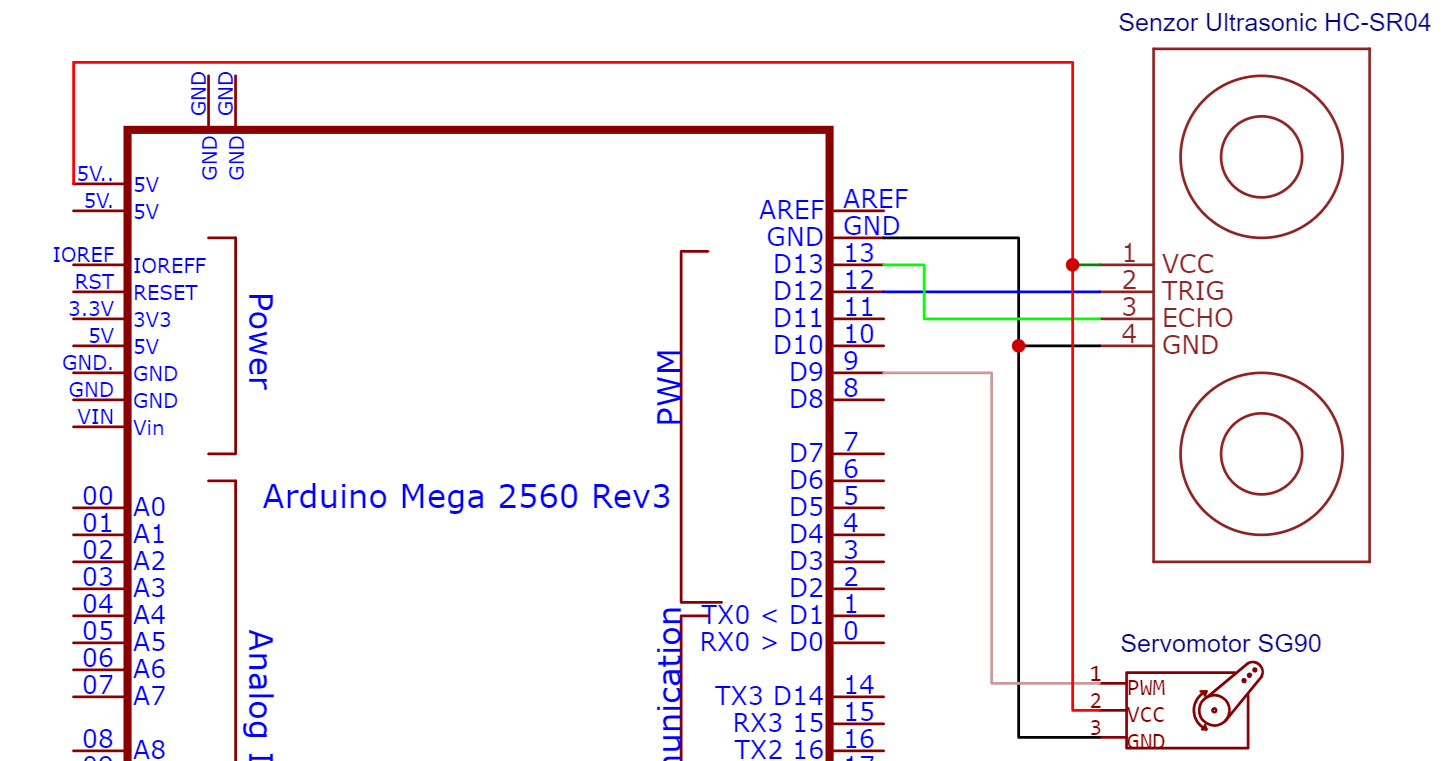
\includegraphics[width=1\textwidth, height=0.6\textwidth]{bachelors_ro/images/conexiune_servo_hcsr04.png}
\caption{Schema de conectare a senzorului ultrasonic și a servomotorului}
\label{fig:conexiune_servo_hcsr04}
\end{figure}

\section{Conectarea ansamblului de alarmă la detectarea gazelor sau a fumului}
Ansamblului de alarmă la detectarea gazelor sau a fumului este format din senzorul MQ2 și un buzzer pasiv. Senzorul este conectat la un pin analogic, acesta oferind date despre concentrația de gaze și fum prezentă în aer. La depășirea unui anumit prag buzzer-ul este activat pentru câteva secunde.

Buzzer-ul este conectat doar la un pin digital împreună cu o rezistență de 100 Ohm și la GND, neavând nevoie de o tensiune de alimentare. Senzorul, în schimb, trebuie conectat și la o tensiune de alimentare de 5 V pe lână pinul analogic și pinul de GND. Totodată, senzorul MQ2 dispune și de un al patrulea pin, DO, ce ar trebui legat la un pin digital pentru a transmite datele înregistrate, dar acest mod este lipsit de acuratețe deci nu va fi folosit. Astfel, în Tabelul \ref{tab:conexiune_mega_mq2_buzzer} sunt prezentați pinii folosiți pentru sistemul de alarmă.

\begin{table}[H]
\caption{Legăturile dintre Arduino Mega, Senzorul MQ2 și Buzzer}
\label{tab:conexiune_mega_mq2_buzzer}
\fontsize{12}{14}\selectfont
\begin{tabular}{|l|c|c|l|c|}
\hline
Arduino Mega & A0 & D29 & 5 V & GND \\ \hline
Senzorul MQ2 & AO & & VCC & GND \\ \hline
Buzzer & & D-IN & & GND \\ \hline
\end{tabular}
\end{table}

Senzorul MQ2 este conectat la un pin analogic ce dispune de un modul de conversie analog-digital. Acesta translatează o tensiune cuprinsă între 0 și 5 V într-o valoare cuprinsă între 0 și 1023. Intervalul acestei valori este dată de faptul că ADC-ul (Analog to digital convertor) este pe 10 biți permițând 1024 de nivele ($2^{10}$), astfel fiecare nivel reprezintă o tensiune de aproximativ 4.88 mV.
Pentru controlul buzzer-ului, microcontroler-ul trimite un semnal dreptunghiular la o frecvență specifică. Această frecvență este folosită pentru a controla tonul sunetului emis de buzzer. Pentru generarea acestei frecvențe se folosește un pin ce dispune de PWM (Pulse Width Modulation).

În Figura \ref{fig:conexiune_mq2_buzzer} este prezentat montajul ansamblului de alamă format din Senzorul MQ2 și Buzzer.

\begin{figure}[H]
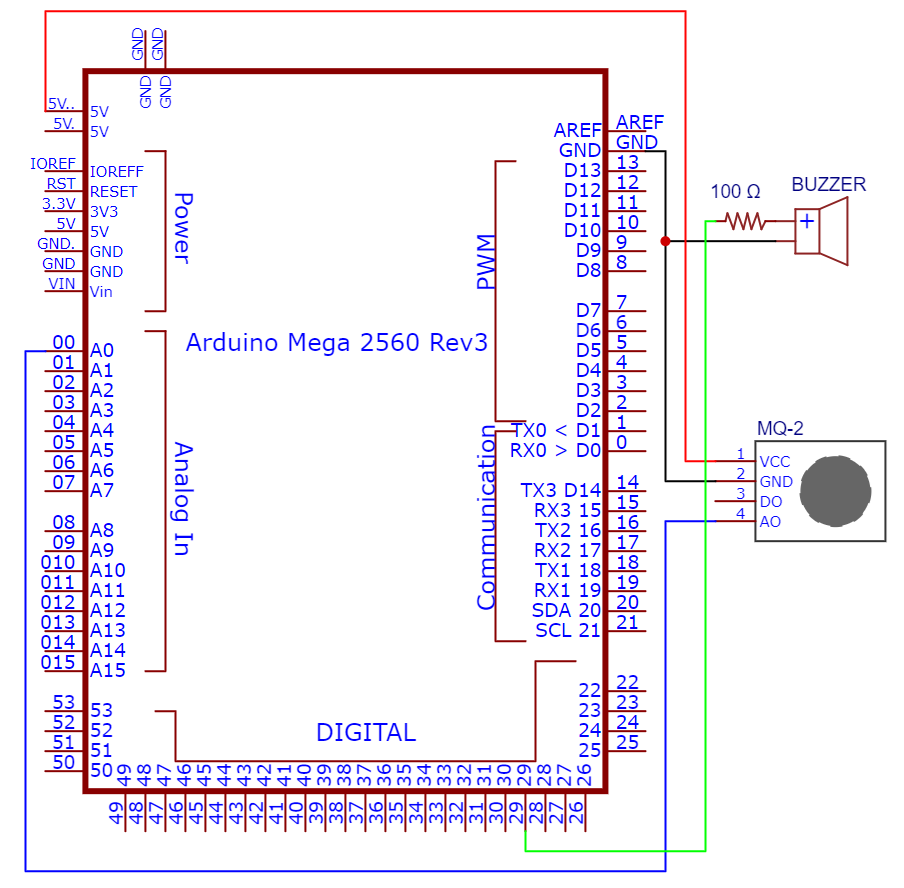
\includegraphics[width=0.7\textwidth, height=0.7 \textwidth]{bachelors_ro/images/conexiune_mq2_buzzer.png}
\caption{Schema de conectare a senzorului de gaz și fum și al buzzer-ului}
\label{fig:conexiune_mq2_buzzer}
\end{figure}

\section{Conectarea Senzorului PIR și al led-ului aferent si al modulului cu fotorezistor și al led-ului aferent}
Primul ansamblu are ca scop aprinderea led-ului în momentul în care senzorul PIR detectează mișcare. Pentru a fi conectat la placa de dezvoltare, led-ul are nevoie de o rezistență de 220 Ohm pe firul de alimentare ce este legat la un pin digital (D26). Rezistența este folistă pentru a limita curentul ce trece prin led pentru a evita arderea acestuia, valoarea este calculată folosind legea lui Ohm ($I=U/R$). Celălalt picior al led-ului este legat la pinul GND. Senzorul PIR dispune de 3 pini: VCC, Dout, GND. Pinul VCC este legat la pinul 5 V de pe placă, pinul de GND la pinul GND al plăcii, iar Dout la pinul digital D4.

Cel de-al doilea ansamblu are ca scop aprinderea led-ului în funcție de nivel de lumină detectat de modulul cu fotorezistor. Led-ul aferent modului este legat în același fel ca și la ansamblul anterior cu mențiunea ca acesta este conectat la pinul D24. Modulul cu fotorezistor dispune de aceeași 3 pini ca și senzorul PIR. Modulul de legătură este similar cu excepția faptului că pinul Dout al modulului este legat la pinul digital D8 al plăcii Arduino.

În figura \ref{fig:conexiune_pir_lum_led} este prezentat montajul final pentru senzorul PIR, modulul cu fotorezistor și led-uri.

\begin{figure}[H]
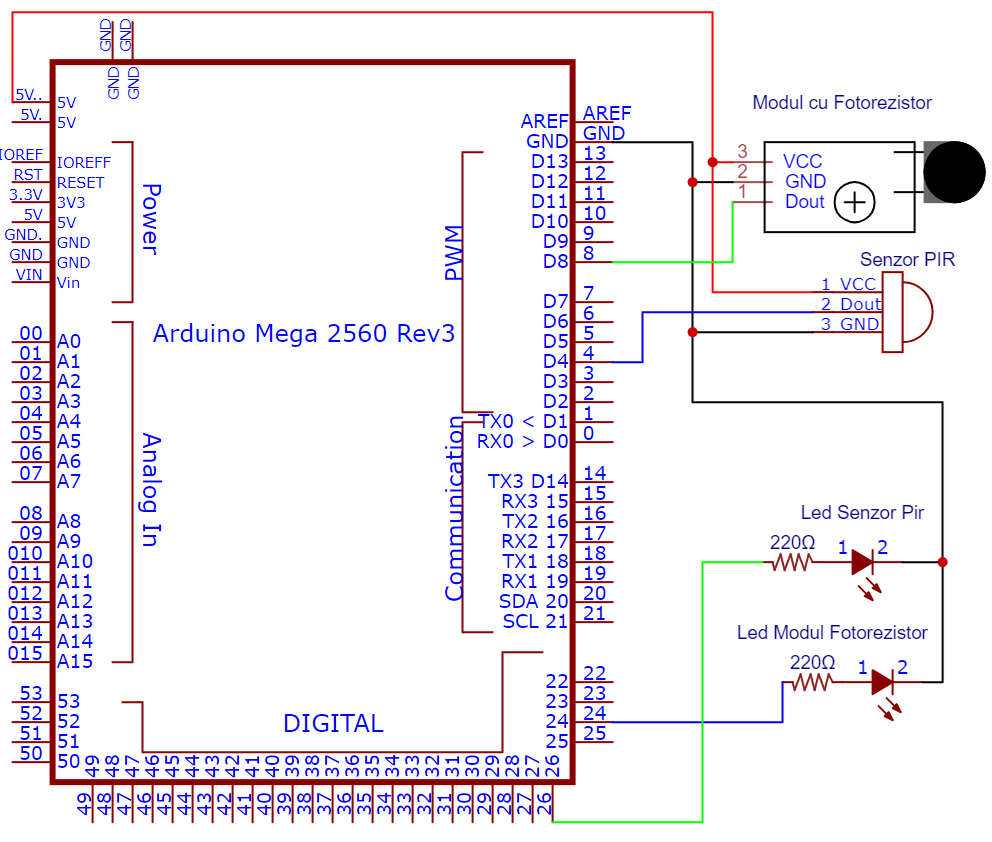
\includegraphics[width=0.8\linewidth]{bachelors_ro/images/conexiune_pir_lum_led.png}
\caption{Schema de conectare a senzorului PIR, a modulului cu fotorezistor și a led-urilor aferent}
\label{fig:conexiune_pir_lum_led}
\end{figure}
\chapter{Arhitectura Software}
\thispagestyle{pagestyle}

Arhitectura software generală a sistemului este alcătuită la rândul ei din trei arhitecturi software separate: arhitectura software pentru placa de dezvoltare Arduino Mega, arhitectura software pentru aplicația mobilă și arhitectura software pentru platforma web/mobile Blynk. În acest capitol ne vom axa doar pe arhitectura generală.

În Figura \ref{fig:arhitectura_soft_general} este prezentată schema bloc a sistemului. Practic, se poate observa funcționarea sistemului într-un ciclu de execuție. Flow-ul de execuție al unui ciclu este următorul: se alimentează sistemul, se inițializază placa, modulele și senzorii, se stabilesc conexiunile cu NodeMCU și modulul de Bluetooth; dacă tot acest setup este efectuat cu succes urmează să introducem un număr la tastatură. Acest număr reprezintă temperatura de prag pe care o dorim în casă. Acest proces de introducere al numărului se termină în momentul în care este apăsată tasta "\#". După introducere, microcontrolerul strânge datele de la senzori, afișează aceste date pe LCD, după care comandă actuatorii (leduri, buzzer, servomotor).

Următorul pas este încercarea de a trimite date prin modulul de Bluetooth către aplicația mobilă de Android. Dacă transmisia a fost realizată cu succes, aplicația va afișa pe ecran datele primite și va aștepta următoarea transmisie lăsând microcontrolerul să execute instrucțiunile rămase. Dacă transmisia eșuează, microcontrolerul ignoră acest fapt continuând setul de instrucțiuni, astfel sistemul nu rămâne blocat.

Apoi, microcontrolerul va încerca să trimită datele către NodeMCU. Dacă comunicarea este realizată cu succes, NodeMCU va trimite datele mai departe către Serverul Blynk, iar acesta le va afișa în interfața platformei. Pe urmă, NodeMCU așteaptă date noi permițând microcontrolerului să execute programul rămas. Dacă comunicarea nu se poate realiza între cele două, microcontrolerul ignoră acest pas și continuă.

Ultima etapă este cea de verificare: dacă palca de dezvoltare este alimentată va continua repetarea acestui ciclu. Astfel, atât timp cât Arduino Mega este alimentată sistemul va executa ciclic aceste etape până la un semnal de reset sau oprirea alimentării.

\begin{figure}[H]
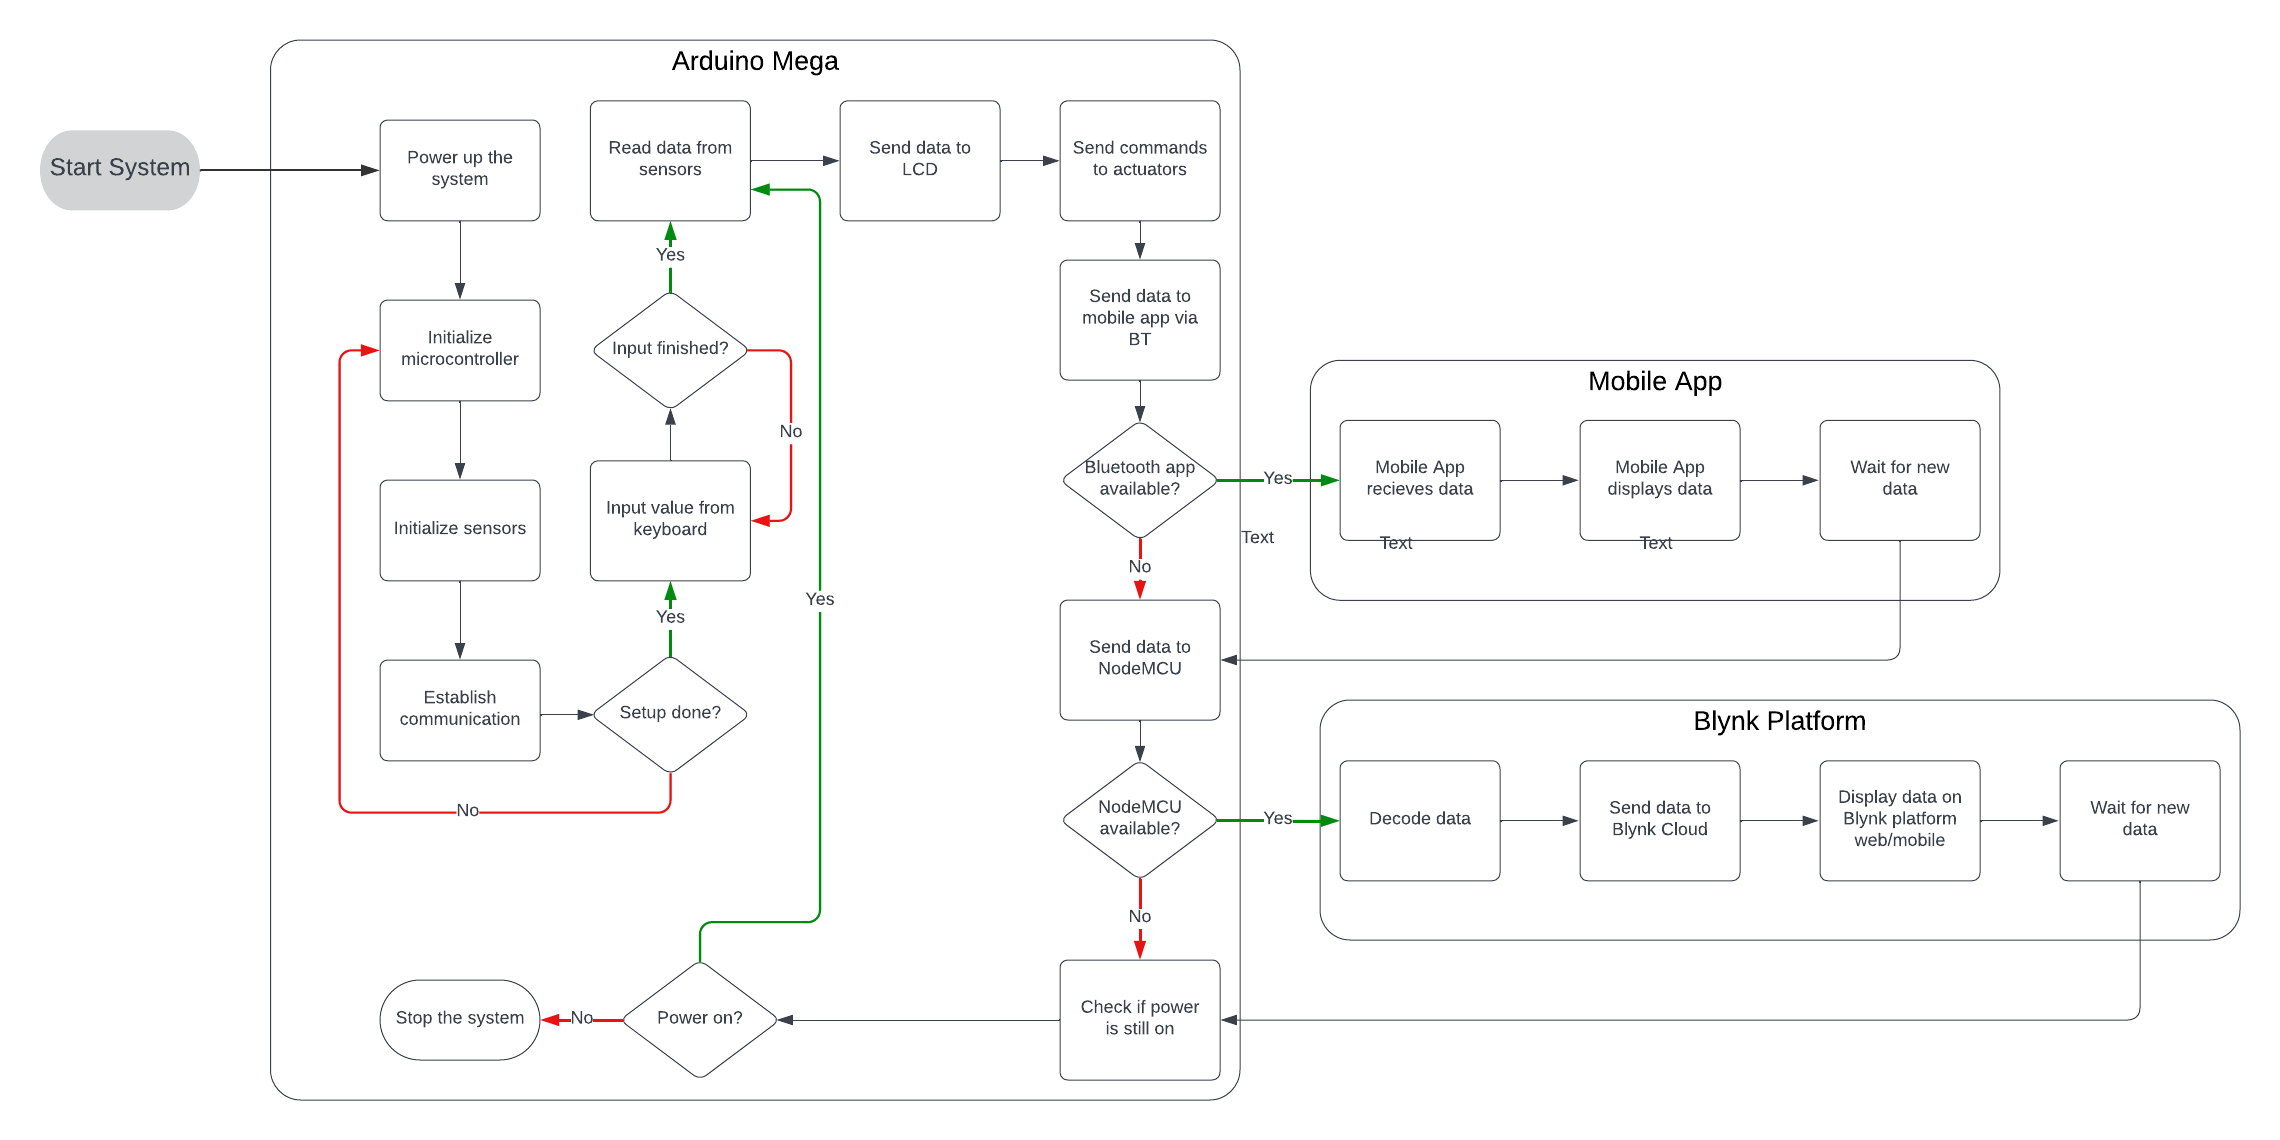
\includegraphics[width=1\textwidth, height=0.6\textwidth]{bachelors_ro/images/arhitectura_soft_general.png}
\caption{Schema software bloc a sistemului}
\label{fig:arhitectura_soft_general}
\end{figure}

\chapter{Implementarea Software pe placa de dezvoltare Arduino Mega}
\thispagestyle{pagestyle}
În acest capitol va fi prezentată în detaliu implementarea software pe placa de dezvoltare Arduino Mega. Microcontroller-ul ATmega2560 face parte din seria AVR produsă de Atmel și reprezintă "creierul" întregului sistem. Acesta va comanda întreaga execuție a codului implementat.

Codul sursă rulat de ATmega2560 este scris în limbajul C++, dar cu câteva modificări aduse specific pentru plăcile de dezvoltare Arduino. Mediul de dezvoltare folosit pentru realizarea codului este Arduino IDE\cite{arduino_ide}. Structura codului este formată din două funcții: \texttt{setup()} ce este apelată o singură dată la începutul execuției și \texttt{loop()} care rulează în continuu până la un reset sau o lipsă de alimnetare.


\section{Implementarea ansamblului de stabilizare a temperaturii}

Pentru a realiza ansamblul de stabilizare a temperaturii este nevoie de următoarele componente: tastatura 4x4, senzorul DHT11, releu pentru controlul becului și releu pentru controlul ventilatorului.

\subsection{Definirea pinilor și inițializarea componentelor}
Pentru a realiza implementarea, avem nevoie două biblioteci predefinite pentru tastatură și senzorul de temperatură:
\begin{code}[H]
\begin{lstlisting}[language=C++]
#include <DHT.h>;
#include <Keypad.h>;
\end{lstlisting}
\caption{Bibliotecile folosite pentru tastatură și senzorul DHT11\cite{lib_key},\cite{lib_dht}}
\label{code:bib_key_dht}
\end{code}

Următorul pas este definirea pinilor la care sunt legate componentele și tipul senzorului DHT deoarece acesta poate fi de două tipuri: DHT11 și DHT 22. Tastatura are un mod propriu de definire a pinilor diferit de celelalte componente datorită bibliotecii folosite. Toate acestea sunt prezentate în Fragmentul \ref{code:def_temp_key_relay}

\begin{code}[H]
\begin{lstlisting}[language=C++]
#define DHTTYPE DHT11
#define DHTPIN 5
#define RELAYPINBEC 11
#define RELAYPINFAN 7

const byte ROWS = 4;
const byte COLS = 4;

char hexaKeys[ROWS][COLS] = {
{'1','2','3','A'},
{'4','5','6','B'},
{'7','8','9','C'},
{'*','0','#','D'}
};

byte rowPins[ROWS] = {53, 51, 49, 47};
byte colPins[COLS] = {45, 43, 41, 39};
Keypad keypad = Keypad(makeKeymap(hexaKeys), rowPins, colPins, ROWS, COLS);
\end{lstlisting}
\caption{Definirea pinilor ansamblului de stabilizare a temperaturii}
\label{code:def_temp_key_relay}
\end{code}

Din codul prezentat în Fragmentul \ref{code:def_temp_key_relay} se observă modul diferit de definire al pinilor folosiți de tastatură. Constantele de la liniile \textit{(6)} și \textit{(7)} definesc numărul de rânduri și coloane. De la linia \textit{(9)} până la linia \textit{(14)} este declarată o matrice de caractere unde fiecare element reprezintă o tastă de pe tastatură. La liniile \textit{(16)} și \textit{(17)} sunt definiți pinii digitali ai plăcii de dezvoltare folosiți de tastatură. Linia de cod \textit{(18)} creează un obiect Keypad. Aceasta mapează tastatura fizică la codul software prin: \texttt{makeKeymap(hexaKeys)} creează harta de taste utilizând matricea \texttt{hexaKeys}; \texttt{rowPins} specifică pinii pentru rândui si \texttt{colPins} specifică pinii pentru coloane; \texttt{ROWS} și \texttt{COLS} specifică dimensiunea matricii. Astfel, tastatura este inițializată.

\begin{code}[H]
\begin{lstlisting}[language=C++]
dht.begin();
pinMode(RELAYPINBEC, OUTPUT);
pinMode(RELAYPINFAN, OUTPUT);
\end{lstlisting}
\caption{Inițializarea senzorului DHT11 și al releelor}
\label{code:init_dht_relay}
\end{code}

Codul din Fragmentul \ref{code:init_dht_relay} se execută în partea de \texttt{setup()} a codului. Senzorul este inițializat automat cu autorul bibliotecii aferente, iar pinii de care sunt legate releele sunt puși în modul OUTPUT pentru a le putea controla utilizând semnale.

\begin{code}[H]
\begin{lstlisting}[language=C++]
 while (!completed) {
    char key = keypad.getKey();
    if (key != NO_KEY) {
      if (key == '#') {
        temperaturaSetata = inputTemp.toFloat(); 
        Serial.println("Temperatura setata:");
        Serial.println(temperaturaSetata);
        completed = true; 
      } else if (isdigit(key)) {
        inputTemp += key;
        Serial.print("Continuati introducerea temperaturii sau apasati tasta # pentru oprire: ");
        Serial.println(inputTemp); 
      }
    }
  }
\end{lstlisting}
\caption{Setarea temperaturii de prag}
\label{code:set_temp}
\end{code}

În Fragmentul \ref{code:set_temp} este prezentat modul în care este setată temperatura de prag. Acesta este executat în partea de \texttt{setup()} deoarece temperatura trebuie introdusă o singură dată la începutul execuției codului.

Cu ajutorul bibliotecii \texttt{Keypad.h} se face citirea tastaturii. Aceasta setează pe rând fiecare rând pe LOW, iar apoi citește starea fiecărui pin de coloană. Dacă o cloană este pe LOW, se detectează în matrice tasta apăsată și este trimisă valoarea acesteia.

Utilizatorul va introduce un număr la tastatură urmat de tasta \# atunci când a terminat de introdus numărul. Acest lucru este realizat cu ajutorul buclei \texttt{while(!completed)} și liniile \textit{(4)} și \textit{(8)} care verifică dacă tasta apăsată este \#. În cazul în care a fost apăsată schimbă valoarea flag-ului \texttt{completed} în \texttt{true} oprind bucla. Dacă a fost apăsată orice altă tastă, valoarea numerică a acesteia este adăugată la stringul \texttt{inputTemp} apoi fiind transformată într-un număr real și stocată în variabila \texttt{tempearturaSetata} conform liniei \textit{(5)}.

\subsection{Logica de funcționare a ansamblului de stabilizare a temperaturii}

Folosind biblioteca menționată anterior (\texttt{DHT.h}), se face citirea senzorului DHT11. Senzorul folosește un singur fir pentru comunicare, iar biblioteca gestionează protocolul de comunicare. Microcontroler-ul trimite un semnal de start către senzor, apoi senzorul răspunde cu un semnal de recunoaștere și încep să transmită valorile înregistrate. Senzorul trimite 40 de biți de date către micrcontroler: 16 biți pentru temperatură (8 pentru partea întreagă, 8 pentru partea fracționară), 16 biți pentru umiditate (8 pentru partea întreagă, 8 pentru partea fracționară) și 8 biți pentru checksum pentru a verifica integritatea datelor.

În fragmentul \ref{code:func_temp} este prezentat modul în care ansamblul funcționează și logica din spatele acestuia.

\begin{code}[H]
\begin{lstlisting}[language=C++]
if(dht.readTemperature() >= temperaturaSetata){
  digitalWrite(RELAYPINFAN, HIGH);
  digitalWrite(RELAYPINBEC, LOW);
  }
  else{
    digitalWrite(RELAYPINFAN, LOW);
    digitalWrite(RELAYPINBEC, HIGH);
  }
\end{lstlisting}
\caption{Codul pe baza căruia funcționează ansamblul de stabilizare a temperaturii}
\label{code:func_temp}
\end{code}

La linia \textit{(1)} din Fragmentul \ref{code:func_temp} se ia decizia dacă va porni becul sau ventilatorul. Funcția \texttt{dht.readTemperature()} returnează valoarea temperaturii în momentul apelului și o compară cu temperatura de prag setată anterior. Dacă temperatura curentă este mai mare ca cea setată se accesează prima ramură a instrucțiunii \texttt{if} și se activează pinul de care este legat releul ventilatorului fiind pus pe \texttt{HIGH}. Altfel, dacă temperatura curentă este mai mică, se intră pe a doua ramură setând pinul releului legat la bec pe \texttt{HIGH}, astfel acesta pornește.

\section{Implementarea ansamblului de alarmă la detectarea gazelor sau a fumului}
Senzorul de gaze și fum și buzzer-ul pasiv sunt componentele folosite pentru a realiza alarma. La detectarea gazelor periculoase sau a fumului, senzorul activează un semnal către buzzer, iar acesta va emite sunet timp de trei secunde.

\subsection{Definirea pinilor și inițializarea componentelor}
Senzorul MQ2 are nevoie de o bibliotecă predefinită, iar buzzer-ul funcționează fără o bibliotecă deoarece funcțiile sale sunt implementate în limbajul specific Arduino. Biblioteca folosită de senzor este \texttt{MQ2.h}\cite{lib_mq2}. Aceasta calibrează senzorul în aer curat pentru a stabili o referință, măsurând rezistența internă. Senzorul citește mai multe valori și face o medie pentru a evita zgomotul și a ridica acuratețea.

Următorul pas este definirea pinilor. Avem nevoie de un pin analogic pentru senzor și de un pin digital pentru buzzer. Conform liniilor \textit{(1)} și \textit{(2)} din Fragmentul \ref{code:init_mq2_buzzer} senzorul este legat la pinul analogic A0 al plăcii, iar buzzer-ul la pinul digital 29. La linia \textit{(4)} este inițializat un obiect de tip MQ2 ce este asociat pinului definit anterior și reprezintă senzorul în sine. Funcția \texttt{mq2.begin()} apelată la linia \textit{(6)} inițializează fizic senzorul și îl calibrează pentru a oferi citiri stabile și corecte.

\begin{code}[H]
\begin{lstlisting}[language=C++]
#define MQ2PIN A0
#define BUZZERPIN 29

MQ2 mq2(MQ2PIN);

mq2.begin();
\end{lstlisting}
\caption{Declararea pinilor pentru senzorul MQ2 și buzzer și inițializarea senzorului}
\label{code:init_mq2_buzzer}
\end{code}

\subsection{Logica de funcționare a ansamblului de alarmă}
La detecția gazelor sau a fumului, buzzer-ul trebuie să se activeze pentru trei secunde. În Fragmentul \ref{code:func_mq2_buzzer} este prezentată implementarea acestei funcționalități. La linia \textit{(1)} este verificat dacă valoarea citită de senzor pentru dioxid de carbon, gaz petrolier lichefiat sau fum este mai mare de prag. În cazul în care condiția este adevărată, este înregistrat timpul curent folosind funcția \texttt{millis()} și este activat buzzer-ul conform liniei \textit{(3)} la o frecvență de 1000 Hz. Flagul \texttt{buzzer\_on\_off} este activat și semnalează ca buzzer-ul este activ. Apoi, la linia \textit{(7)} este verificat dacă au trecut trei secunde de la activarea buzzerului. În cazul în care au trecut buzzer-ul este oprit folosind \texttt{noTone(BUZZERPIN)}.

Funcția \texttt{millis()} este o funcție integrată în Arduino și cronometrează timpul trecut de la rularea acelei linii. Astfel, cu ajutorul acestei funcții evităm folosirea funcției \texttt{delay()} ce ar crea o întârziere în întreg sistemul și nu doar în cadrul acestui ansamblu.

\begin{code}[H]
\begin{lstlisting}[language=C++]
  if(mq2.readCO() || mq2.readLPG() || mq2.readSmoke() > 100){
    buzzerStart = millis();
    tone(BUZZERPIN, 1000); 
    buzzer_on_off = true;
  }
  else
    if(buzzer_on_off &&(millis() - buzzerStart >= intervalBuzzer)){
      noTone(BUZZERPIN);
      buzzer_on_off = false;
  }
}
\end{lstlisting}
\caption{Codul pe baza căruia funcționează ansamblul de alarmă}
\label{code:func_mq2_buzzer}
\end{code}

\section{Implementarea senzorului de presiune barometrică și a display-ului LCD cu ajutorul protocolului I2C}
Atât senzorul BMP280, cât și LCD-ul folosesc protocolul I2C pentru a comunica cu placa de dezvoltare Arduino Mega. Astfel, avem nevoie de adresele lor de memorie pentru a realiza conexiunea.

\subsection{Inițtializarea componentelor}
LCD-ul utilizează biblioteca \texttt{LiquidCrystal\_I2C.h}\cite{lib_lcd}, iar senzorul folosește biblioteca \texttt{Adafruit\_BMP280.h}\cite{lib_bmp280}. Ambele componente necesită biblioteca \texttt{Wire.h}\cite{lib_wire} pentru a comunica prin protocolul I2C. Biblioteca pentru display realizează conexiunea dintre modulul I2C și LCD-ul propoiu zis. Modulul interpretează comenzile și le transformă într-un format accesibil pentru display. Biblioteca senzorului ajută la transformarea datelor înregistrate de acesta folosind formule de calibrare. Biblioteca \texttt{Wire.h} este folosită pentru a realiza comunicarea. Aceasta inițializează transmisia către adresa specificată, apoi folosind un buffer transmite datele.


Următorul pas este să inițializăm componentele cu adresele la care se află acestea.

\begin{code}[H]
\begin{lstlisting}[language=C++]
LiquidCrystal_I2C lcd(0x27,16,2);
Adafruit_BMP280 bmp;

void setup(){
lcd.init();
lcd.clear();
lcd.backlight();

bmp.begin(0x76) ;
}
\end{lstlisting}
\caption{Inițializarea LCD-ului și a senzorului BMP280}
\label{code:init_lcd_bmp}
\end{code}

În Fragmentul \ref{code:init_lcd_bmp} la linia \textit{(1)} este inițializat un obiect LCD la adresa 0x27 din memorie, 16 reprezintă numărul de caracter de pe un rănd, iar 2 numărul de rânduri. Senzorul BMP 280 se află la adresa de memorie 0x76 conform liniei \textit{(9)}. Liniile \textit{(5)},\textit{(6)} și \textit{(7)} au ca scop inițializarea fizică a display-ului acestea golind ecranul de orice caracter și setând lumina de fundal.

\subsection{Codul pentru afișarea datelor pe display-ul LCD}
Display-ul LCD afițează datele primite de la senzorul de temperatură și umiditate (DHT11), senzorul de presiune atmosferică și altitudine (BMP280) și senzor de gaze și fum (MQ2). Deoarece dimensiunea datelor este mare și LCD-ul poate afișa doar 32 de caractere simultan, acesta trece prin trei stări separate: prima în care afișează datele de la DHT11, a doua în care afișează datele de la BMP280 și a treia în care afișează datele de la MQ2. Aceste stări sunt executate ciclic.

În Fragmentul \ref{code:func_lcd} sunt prezentate stările prin care trece LCD-ul. Pentru început, la linia \textit{(3)} se verifică cu ajutorul funcției \texttt{millis()} dacă au trecut cele 3 secunde pentru a schimba afișajul. Ecranul trebuie golit înainte de fiecare afișaj pentru a nu exista disfuncții. Apoi, fiecare stare apelează o funcție ce afișează pe display, datele citie de la senzorul aferent stării. Starea 0 este pentru senzorul de temperatură și umiditate (\textit{(7),(8)}), starea 1 este pentru senzorul de gaze și fum (\textit{(9),(10}) și starea 3 este pentru senzorul de presiune și altitudine (\textit{(11),(12)}). Apoi, variabilei \texttt{displayState} îi este atribuită o nouă stare folosind clasa de resturi a numărului trei, adică zero, unu și doi, asigurând ciclicitatea execuției formând o buclă.

\begin{code}[H]
\begin{lstlisting}[language=C++]
const long updateInterval = 5000;

if (millis() - lastDisplayLCD >= intervalLCD){
    lastDisplayLCD = millis(); 
    lcd.clear(); 

    if (displayState == 0){
      displayDHTReadings();
    }else if (displayState == 1){
      displayMQ2Readings();
    }else if (displayState == 2){
      displayBMPReadings();
    }

    displayState = (displayState + 1) % 3; //ca sa trecem circular prin cele trei stari pt lcd
  }
\end{lstlisting}
\caption{Codul pentru afișarea ciclică a datelor pe LCD }
\label{code:func_lcd}
\end{code}

Cele trei funcții \texttt{displayDHTReadings()}, \texttt{displayMQ2Readings()} și \texttt{displayBMPReadings()} sunt similare, astfel în Fragmentul \ref{code:func_bmp_disp} este prezentată doar funcția \texttt{displayBMPReadings()}.

Funcția este de tip \texttt{void} deoarece nu trebuie să returneze nimic, ci doar să printeze pe LCD. În variabilele \texttt{pressure} și \texttt{altitude} sunt stocate valorile citite de către senzor cu ajutorul funcțiilor predefinite oferite de bibliotecă. Apoi, pe primul rând al display-ului începând cu poziția 0 este afișată valoarea presiunii (liniile \textit{(5)-(8)}). La linia \textit{(10)} se trece la cel de-al doilea rând al display-ului la poziția 0 pentru a afișa în mod similar și valoarea altitudinii.

\begin{code}[H]
\begin{lstlisting}[language=C++]
void displayBMPReadings() {
float pressure = bmp.readPressure() * 0.000145038; //transformare Pa -> psi
float altitude = bmp.readAltitude(1020);

lcd.setCursor(0, 0);
lcd.print("Pres: ");
lcd.print(pressure);
lcd.print(" PSI");

lcd.setCursor(0, 1);
lcd.print("Alt: ");
lcd.print(altitude);
lcd.print(" m");
}
\end{lstlisting}
\caption{Afișarea datelor primite de la BMP280}
\label{code:func_bmp_disp}
\end{code}

\section{Implementarea ansamblului de deschidere automată a ușii}
Acest ansamblu este format din senzorul ultrasonic HC-SR04 și micro servomotorul SG90. La detecția unei persoane în proximitatea sa, senzorul comandă un semnal către servomotor pentru a acționa ușa de care este legat printr-o mișcare de 90 de grade. Ușa rămâne deschisă timp de 10 secunde, iar dacă după acest interval nu mai este detectată prezența unei persoane, acest execută o altă mișcare de 90 de grade revenind la poziția inițială.

\subsection{Definirea pinilor și inițializarea componentelor}
În Fragmentul \ref{code:init_servo_hcsr} putem observa că senzorul are nevoie de doi pinii digitali pentru a funcționa: ECHO și TRIG. Sunt folosiți pentru aceasta pinii digitali 12 și 13. În \texttt{setup()} pinul TRIG este setat ca și ieșire (\texttt{OUTPUT}) pentru că acesta emite o undă sonoră, iar dacă aceasta se lovește de un obiect este reflectată și recepționată de pinul ECHO, motiv pentru care este setat pe intrare (\texttt{INPUT}).

Servomotrul are nevoie de biblioteca \texttt{Servo.h} pentru a funcționa \cite{lib_servo}. Este creat un obiect de tip Servo, iar în \texttt{setup()} îi este atașat pinul digital 9 ce dispune de PWM. Biblioteca ajustează lățimea impulsului PWM și modifică poziția servomotorului pe baza duratei impulsului.

\begin{code}[H]
\begin{lstlisting}[language=C++]
#include <Servo.h>

#define TRIGPIN 12
#define ECHOPIN 13
#define SERVOPIN 9

Servo myServo;

void setup(){
pinMode(TRIGPIN, OUTPUT);
pinMode(ECHOPIN, INPUT);

myServo.attach(SERVOPIN);
}
\end{lstlisting}
\caption{Definirea pinilor și inițializarea servomotorului și senzorului ultrasonic}
\label{code:init_servo_hcsr}
\end{code}

\subsection{Logica de funcționare a ansamblului de deschidere automată a ușii}
Funcția \texttt{pulseIn(ECHOPIN, HIGH)} măsoară durata în microsecunde în care semnalul pe pinul ECHO este pe \texttt{HIGH}, indicând timpul necesar pentru ca undele sonore să parcurgă drumul până la un obiect și înapoi. Pentru a calcula distanța avem nevoie de durata de timp calculată anterior și viteza sunetului în aer (0.0343 cm/microsecundă). Astfel, folosind formula \ref{eq:distance} putem calcula distanța la care se află obiectul.

La linia \textit{(4)} se verifică dacă senzorul detectează un obiect la o distantă de maxim 10 cm și folosind funcția \texttt{millis()} deschide ușa mutând servomotorul la 90 de grade timp de 10 secunde. Apoi după 10 secunde, ușa rămâne deschisă dacă senzorul detectează o prezență, dacă nu, revine la poziția inițială de 0 grade.

\begin{code}[H]
\begin{lstlisting}[language=C++]
  duration = pulseIn(ECHOPIN, HIGH);
  distance = (duration * 0.0343) / 2; // 0.0343 cm/micros (343 m/s) = viteza sunetului in aer
  
  if (distance < 10 && millis() - lastServoMove >= intervalUltra){ 
    myServo.write(90);
    lastServoMove = millis(); 
  }

  if (millis() - lastServoMove < intervalUltra){
    myServo.write(90); 
  }
  else{
    myServo.write(0);
  }
\end{lstlisting}
\caption{Mișcarea servomotorului comandată de senzorul ultrasonic}
\label{code:func_servo_hcsr}
\end{code}

\begin{equation}
\label{eq:distance}
\text{Distanța} = \frac{\text{Viteza sunetului} \times \text{Durata de zbor a undei}}{2}
\end{equation}

\section{Implementarea Senzorului PIR și al led-ului aferent}
\label{sec:senzor_pir_led}
Acest ansamblu are ca scop aprinderea unui led în momentul în care senzorul PIR detectează mișcare.

Conform Fragmentului \ref{code:init_pir_led}, senzorul trimite către pinul digital 4 valoarea 1 sau 0, fiind pus pe modul intrare. Pinul aferent led-ului este setat în modul ieșire deoarece acesta trimite un semnal care aprinde led-ul. Astfel, se realizează comanda dintre senzor și led.

\begin{code}[H]
\begin{lstlisting}[language=C++]
#define PIRPIN 4
#define LEDPIRPIN 26

setup(){
pinMode(PIRPIN, INPUT);
pinMode(LEDPIRPIN, OUTPUT);
}
\end{lstlisting}
\caption{Definirea pinilor și inițializarea senzorului și a led-ului}
\label{code:init_pir_led}
\end{code}

Logica de funcționare este simplă deoarece senzorul PIR dispune de setarea timpului în care semnalul trimis are valoare 1 și distanța la care acesta acționează folosind două potențiometre atașate pe senzor. Cât timp senzorul trimite valoarea 1, adică detectează mișcare, led-ul este comandat să se aprindă. Când senzorul nu detectează mișcare și comută pe valoarea 0, led-ul se stinge. Acest principiu poate fi urmărit în Fragmentul \ref{code:func_pir_led}

\begin{code}[H]
\begin{lstlisting}[language=C++]
if(digitalRead(PIRPIN)==1){
    digitalWrite(LEDPIRPIN,HIGH);
  }
  else
  {
    digitalWrite(LEDPIRPIN,LOW);
  }
\end{lstlisting}
\caption{Comandarea led-ului cu ajutorul senzorului PIR}
\label{code:func_pir_led}
\end{code}

\section{Implementarea modulului cu fotorezistor și al led-ului aferent}
Rolul acestui ansamblu este de a controla un led în funcție de nivelul de lumină detectat de fotorezistor. Astfel, dacă nivelul de lumină este scăzut modulul comandă led-ul să fie aprins.

Modulul are nevoie de un pin digital la care să trimită date, iar led-ul de un pin digital prin care să fie trimis un semnal care să îl aprindă. În Fragmentul \ref{code:init_lum_led} se observă că pentru modul se folosește pinul digital 8 setat pe modul intrare, iar pentru led pinul 24 setat pe ieșire.

\begin{code}[H]
\begin{lstlisting}[language=C++]
#define SLUMINAPIN 8
#define LEDLUMINAPIN 24

setup(){
pinMode(SLUMINAPIN, INPUT);
pinMode(LEDLUMINAPIN, OUTPUT);
}
\end{lstlisting}
\caption{Comandarea led-ului cu ajutorul senzorului PIR}
\label{code:init_lum_led}
\end{code}

Logica de funcționare este similară cu cea prezentată în subcapitolul \ref{sec:senzor_pir_led}. Modulul dispune de un potențiometru ce permite ajustarea sensibilității la lumină. Diferența majoră este că led-ul se activează atunci când modulul emite valoarea 1, adică fotorezistorul nu detectează lumină. Modulul trimite valoarea 0 când nivelul luminii a trecut de pragul setat cu ajutorul potențiometrului și astfel led-ul se stinge. Acest mod de funcționare este prezentat în Fragmentul \ref{code:func_lum_led}.

\begin{code}[H]
\begin{lstlisting}[language=C++]
if(digitalRead(SLUMINAPIN) == 0){
digitalWrite(LEDLUMINAPIN,LOW);
}
else {
digitalWrite(LEDLUMINAPIN,HIGH);
}
\end{lstlisting}
\caption{Comandarea led-ului cu ajutorul modulului cu fotorezistor}
\label{code:func_lum_led}
\end{code}

\section{Implementarea comunicării seriale între Arduino Mega, NodeMCU și modulul Bluetooth}

Placa de dezvoltare Arduino Mega comunică serial atât cu modulul WiFi NodeMCU, cât și cu modulul Bluetooth HC-05. Fiecare comunicare se face individual printr-un alt canal.

Comunicarea dintre Arduino Mega și modulul HC-05 se realizează folosind interfața UART 0 fiind folosiți pinii 0 (RX0) și 1 (TX0) ai plăcii. Acești pini nu trebuie declarați în cod deoarece este suficientă doar legătura hardware. Comunicarea trebuie inițializată folosind funcția \texttt{Serial.begin(9600)} ce este implementată în limbajul folosit de Arduino, nefiind necesară o bibliotecă specifică.

Pentru comunicarea dintre Arduino Mega și modulul NodeMCU se folosește interfața UART 3. Astfel la nivel de hardware s-a realizat o conexiune între pinii 14 (TX3) și 15 (RX3) la pinii dedicați ai modulului. În mod echivalent cu paragraful anterior și această conexiune trebuie inițializată prin apelul funcției \texttt{Serial3.begin(9600)} în partea de \texttt{setup()}.

Arduino Mega trimite către modulul Bluetooth un șir de caractere format din citirile tuturor senzorilor. Astfel, șirurile de caractere returnate de funcțiile \texttt{readDHTSensor()}, \texttt{readMQ2Sensor()}, și \texttt{readBMPSensor()} sunt concatenate în String-ul \texttt{dataStringBt} fiind separate de caracterul new line \texttt{\textbackslash n} pentru vizibilitate. Apoi, pentru a trimite efectiv datele către modul, se apelează funcția \texttt{Serial.println()} care are ca argument șirurl de caractere \texttt{dataStringBt} pe care dorim sa îl trimitem. Caracterul \texttt{\$} este folosit pentru a semnala sfârșitul șirului.

\begin{code}[H]
\begin{lstlisting}[language=C++]
String dataStringBt = readDHTSensor() + "\n" + readMQ2Sensor() + "\n" + readBMPSensor() + "$";
Serial.println(dataStringBt);
\end{lstlisting}
\caption{Trimiterea serială a datelor către modulul Bluetooth HC-05}
\label{code:func_uart_bt}
\end{code}

Cele trei funcții de citire a datelor prezente în Fragmentul \ref{code:func_uart_bt} funcționează în mod similar. Acestea sunt de tip \texttt{String} și citesc datele de la senzori și le transformă din numere reale în șiruri de caractere. În Fragmentul \ref{code:func_read_dht} este prezentată funcția \texttt{readDHTSensor()} care citește datele de la senzorul DHT11 și returnează datele sub formă de șir de caractere. În mod asemănător sunt tratate și funcțiile \texttt{readMQ2Sensor()} și \texttt{readBMPSensor()}.

\begin{code}[H]
\begin{lstlisting}[language=C++]
String readDHTSensor() {
float humidity = dht.readHumidity();
float temperature = dht.readTemperature();

if (isnan(humidity) || isnan(temperature)) {
return "Nu se poate citi DHT11";
}

return "Temperature: " + String(temperature) + "\nHumidity: " + String(humidity);
}
\end{lstlisting}
\caption{Funcția de citire a datelor de la senzorul DHT11 și transformarea acestora în șiruri de caractere}
\label{code:func_read_dht}
\end{code}

Datele trimise către modulul NodeMCU sunt reprezentate tot de citirile senzorilor, doar că în acest caz fiecare valoare este transformată în șir de caractere individual și este separată de un spațiu pentru a permite modului o decodare mai facilă.

\begin{code}[H]
\begin{lstlisting}[language=C++]
String data_esp= String(dht.readHumidity())+" "+String(dht.readTemperature())+" "+String(mq2.readCO()*(5/1023.0))+" "+String(mq2.readLPG()*(5/1023.0))+" "+String(mq2.readSmoke()*(5/1023.0))+" "+String(bmp.readAltitude(1020))+" "+String(bmp.readPressure()* 0.000145038);
Serial3.println(data_esp);
\end{lstlisting}
\caption{Trimiterea serială a datelor către modulul NodeMCU}
\label{code:func_uart_esp}
\end{code}
\chapter{Implementarea Software pe Modulul NodeMCU ESP8266 și platforma Blynk}
\thispagestyle{pagestyle}

În acest capitol este prezentat modul în care modulul NodeMCU primește datele de la placa de dezvoltare Arduino Mega și le transmite prin WiFi către platforma Blynk.

NodeMCU este o placă de dezvoltare ce are incorporat un modul ESP8266 de WiFI și chip de conversie USB CH340 \cite{nodemcu_ard}. Aceasta este programabilă utilizând Arduino IDE și acceptă același limbaj de programare bazat pe C++ folosit și de Arduino Mega.

Modulul ESP8266 oferă o soluție ideală pentru proiectele ce includ sistemele încorporate, oferind o conexiune facilă la WiFi. Acesta este comandat de o unitate centrală de procesare (CPU) Tensilica L106. Acest procesor dispune de o arhitectură pe 32 de biți de tip RISC ce poate ajunge până la o frecvență de 160 MHz, dar în același timp să și rămână eficient din punct de vedere al consumului\cite{nodemcu_datasheet}.

\section{Recepția datelor de la Arduino Mega}

Modulul NodeMCU primește datele de placa Arduino Mega prin intermediul comunicării seriale. Sunt folosiți pinii predefiniți de interfață UART
RX și TX. Această conexiune nu trebuie definită în cod deoarece s-a executat deja hardware conectând fire între cele două interfețe UART.

Pentru a inițializa conexiunea serială, în secțiunea \texttt{setup()} este apelată funcția \texttt{Serial.begin(9600)}. Argumentul \texttt{9600} este folosit pentru a seta rata de transfer (Baud Rate) și este identică cu cea setată pe Arduino Mega pentru a nu exista erori în transmisie.

\begin{code}[H]
\begin{lstlisting}[language=C++]
if (Serial.available()) {
    String line = Serial.readStringUntil('\n');
    float valuesFromSen[7]; 
    int start = 0;
    for (int i = 0; i < 7; i++) {
      int spaceIndex = line.indexOf(' ', start);
      if (spaceIndex == -1) spaceIndex = line.length(); // cand nu mai sunt spatii merge pana la sfrasit
      String subStr = line.substring(start, spaceIndex);
      valuesFromSen[i] = subStr.toFloat();
      start = spaceIndex + 1;
    }
\end{lstlisting}
\caption{Decodarea șirului primit de la Arduino Mega}
\label{code:decode_data_esp}
\end{code}

Primul pas în decodarea datelor trimise este citirea de pe interfața serială. Acest lucru se întâmplă la linia \textit{(1)} unde este verificat dacă interfața este disponibilă. Apoi, dacă aceasta este activă, se citesc date folosind funcția \texttt{Serial.readStringUntil('\textbackslash n')} până la înâlnirea caracterului \texttt{\textbackslash n}, iar datele citite sunt stocate în variabila \texttt{line} de tip șir de caractere. Datele primite sunt formatate astfel încât să fie despărțite printr-un caracter "spațiu" (' '), iar setul de date să se termine cu \texttt{\textbackslash n}, astfel se poate identifica momentul în care sunt trimise date noi.

Vectorul \texttt{valuesFromSen[7]} are o dimensiune de 7 elemente deoarece sunt trimise 7 valori aparținând senzorilor de pe placa Arduino Mega. Variabila \texttt{start} este folosită pentru a înregistra indexul de început al porțiunii ce este decodată.

La linia \textit{(5)} din Fragmentul \ref{code:decode_data_esp} se găsește o bulcă \texttt{for} ce este iterată de 7 ori pentru fiecare valoare ce trebuie decodată. În variabila \texttt{spaceIndex} va fi rețiuntă poziția caracterului spațiu găsit în șirul de caractere \texttt{line} începând de la poziția indicată de \texttt{start}. Dacă nu este găsit niciun caracter spațiu, \texttt{indexOf} va returna -1, ceea ce înseamnă că am ajuns la ultima valoare de decodat și setăm \texttt{spaceIndex} cu lungimea șirului.

Astfel, folosind indexul caracterului spațiu și indexul de start al subșirului, este extrasă porțiunea ce conține o valoare transmisă și se stochează în șirul de caractere \texttt{subStr} folosind funcția \texttt{substring()}. Porțiunea extrasă este apoi convertită în număr real și stocată în vectorul \texttt{valuesFromSen[7]}, iar variabila \texttt{start} este setată la următoare poziție după \texttt{spaceIndex} pentru a continua decodarea.

\section{Configurarea interfeței de afișare pe platforma Blynk}
\label{configurare_blynk}
Pentru a trimite date către platforma Blynk, este necesar să creăm un template pe platformă alegând un nume, modulul folosit și tipul de conexiune.

\begin{figure}[H]
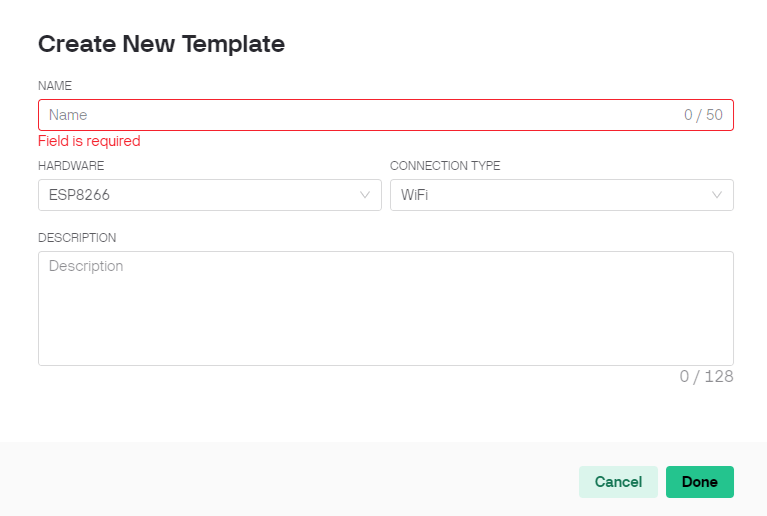
\includegraphics[width=0.7\linewidth]{bachelors_ro/images/blynk_template.png}
\caption{Crearea unui template pe platforma Blynk \cite{templ_blynk}}
\label{fig:template_blynk}
\end{figure}

După ce template-ul a fost creat, trebuie setate data stream-urile. Acestea reprezintă pini virtuali unde sunt transmise datele de pe modulul NodeMCU către platforma și sunt stocate individual. Acești pini pot fi configurați setând tipul de date primit și valoarea maximă ce poate fi reținută. Acest aspect este prezentat în Figura \ref{fig:data_stream_blynk}.

\begin{figure}[H]
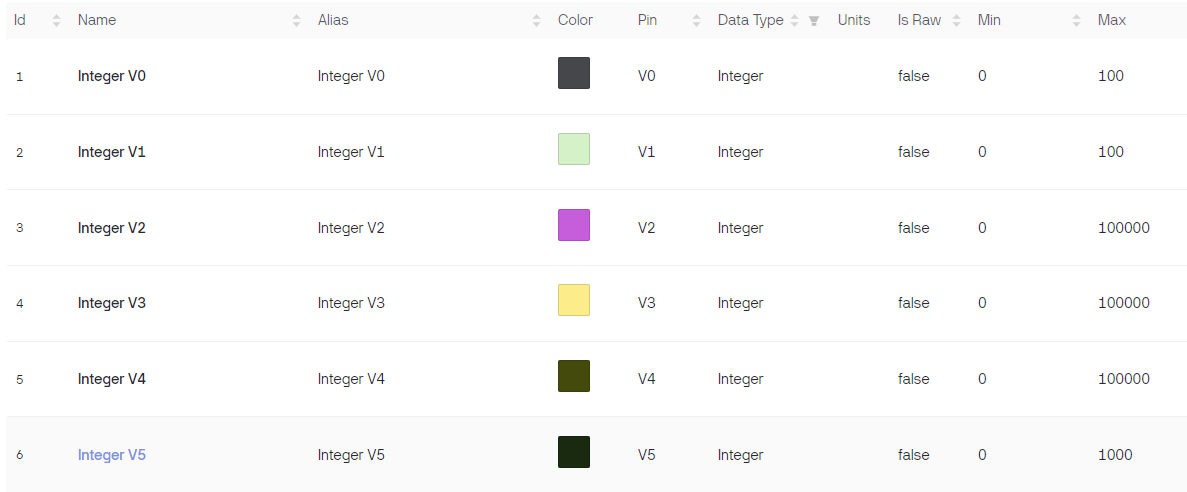
\includegraphics[width=0.9\textwidth, height=0.4\textwidth]{bachelors_ro/images/data_streams_blynk.png}
\caption{Configurarea data stream-urilor pe platforma Blynk \cite{templ_blynk}}
\label{fig:data_stream_blynk}
\end{figure}

Odată ce există un mod de recepționare a datelor pe platformă trebuie creată o interfață pentru a fi afișate. Astfel în secțiunea "Web Dashboard" pot fi adăugate elemente grafice ce afișează datele de la pinii virtuali. Platforma Blynk dispune de o varietate de widget-uri de afișaj, dar pentru acest proiect a fost ales widget-ul de tip indicator ("Gauge").

Acest gauge trebuie configurat la rândul său conform Figurii \ref{fig:config_gauge}. Trebuie să introducem un nume pentru widget și să alegem pinul virtual de la care acesta afișează datele.

\begin{figure}[H]
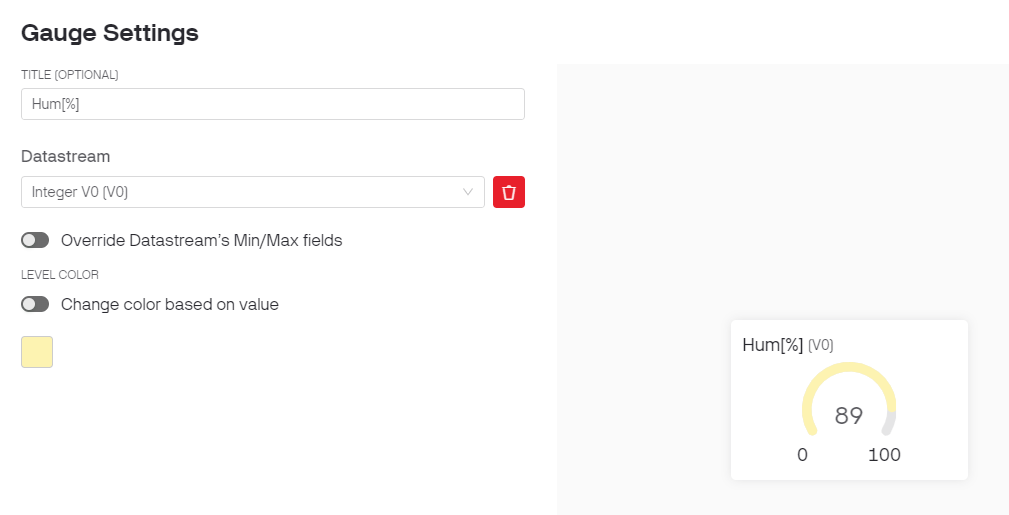
\includegraphics[width=0.8\linewidth]{bachelors_ro/images/config_gauge.png}
\caption{Configurarea gaguge-ului pentru un anumit pin virtual\cite{templ_blynk}}
\label{fig:config_gauge}
\end{figure}

După configurarea mai multor widget-uri pentru fiecare valoarea trimisă de modulul NodeMCU, în secțiunea "Devices" se poate observa interfața web finală obținută. (\ref{fig:interfata_blynk}).

\begin{figure}[H]
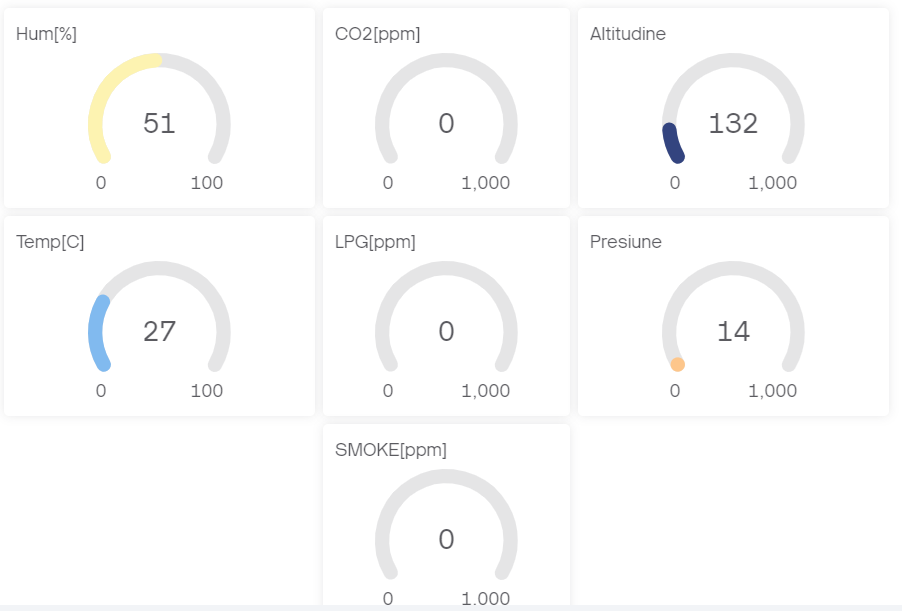
\includegraphics[width=0.7\linewidth]{bachelors_ro/images/interfata_blynk.png}
\caption{Interfața Web Blynk \cite{templ_blynk}}
\label{fig:interfata_blynk}
\end{figure}

Pentru a crea interfața mobile folosind aplicația Blynk sunt urmăriți aceeași pași menționați anterior. Interfața de pe platforma mobile Blynk se poate observa în Figura \ref{fig:interfata_blynk_mobile}.

\begin{figure}[H]
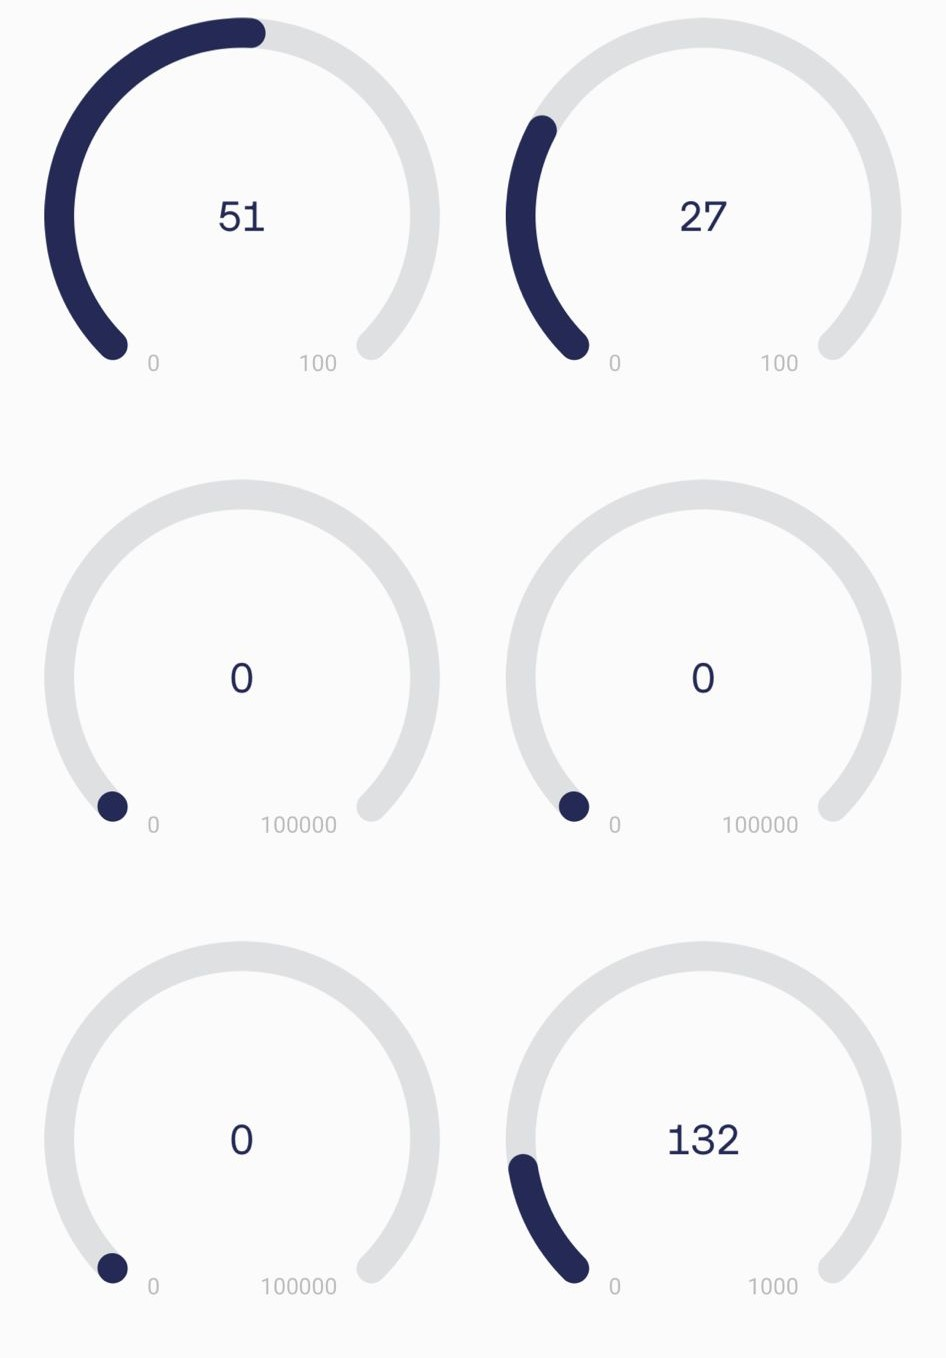
\includegraphics[width=0.4\linewidth]{bachelors_ro/images/interfata_blynk_mobile.jpg}
\caption{Interfața Mobile Blynk\cite{templ_blynk}}
\label{fig:interfata_blynk_mobile}
\end{figure}

\section{Transmiterea datelor către platforma Blynk}
După ce interfețele au fost configurate, următorul pas este trimiterea datelor prin WiFi către platforma Blynk. Pentru realizarea acestei transmisi avem nevoie de două biblioteci specifice: \texttt{ESP8266WiFi.h} \cite{lib_esp} și \texttt{BlynkSimpleEsp8266.h} \cite{lib_blynk}. Aceste biblioteci oferă posibilitatea de conexiune la WiFi a modulului și conectare la platforma Blynk.

Pentru a conecta modulul NodeMCU la dispozitivul creat pe platformă, avem nevoie de câteva informații cheie: id-ul template-ului, numele template-ului, cheia de autentificare, SSID-ul rețelei la care dorim să ne conectăm și parola acesteia. Acestea sunt transmise prin cod conform Fragmentului \ref{code:token_blynk} oferit de platforma Blynk \cite{blynk_browser}, însă au fost criptate din motive de securitate.

\begin{code}[H]
\begin{lstlisting}[language=C++]
#define BLYNK_TEMPLATE_ID           "TMPxxxxxx"
#define BLYNK_TEMPLATE_NAME         "Device"
#define BLYNK_AUTH_TOKEN            "AuthToken"

char ssid[] = "NetworkName";
char pass[] = "Password";
\end{lstlisting}
\caption{Declararea informațiilor pentru conectarea la dispozitivul Blynk \cite{blynk_browser}}
\label{code:token_blynk}
\end{code}

Apoi, pentru a inițializa conexiunea, în \texttt{setup()} este apelată funcția \texttt{Blynk.begin(BLYNK\_AUTH\_TOKEN, ssid, pass)}. Argumentele acesteia sunt datele declarate anterior și indică device-ul Blynk la care trebuie să ne conectăm și rețeaua pe care trebuie să o folosim. 

În urma conectării la rețea și la dispozitivul Blynk, datele decodificate de NodeMCU sunt trimise către pinii virtuali definiți în subcapitolul \ref{configurare_blynk}. În Fragmentul \ref{code:send_data_to_blynk} este prezentată metoda de transmitere a datelor. Funcția \texttt{Blynk.run()} asigură menținerea conexiunii și sincronizarea între modulul NodeMCU și platforma Blynk. Bucla \texttt{for} este iterată de 7 ori pentru fiecare valoare decodificată și pentru fiecare pin virtual. Cu ajutorul indexului \texttt{i} fiecărui pin virtual îi este desemnată o valoare decodificată folosind funcția \texttt{Blynk.virtualWrite()}. Acest ansamblu de cod se execută ciclic în funcția \texttt{loop()} și astfel transmiterea datelor de la NodeMCU la platforma web și mobile Blynk este realizată cu succes.

\begin{code}[H]
\begin{lstlisting}[language=C++]
Blynk.run();

for (int i = 0; i < 7; i++) {
    Blynk.virtualWrite(V0 + i, valuesFromSen[i]);
}
\end{lstlisting}
\caption{Trimiterea datelor către pinii vituali}
\label{code:send_data_to_blynk}
\end{code}

\chapter{Implementarea aplicației mobile}
\thispagestyle{pagestyle}

În acest capitol este prezentat modul de implementare și funcționare al aplicației mobile ce comunică cu placa de dezvoltare Arduino Mega. Aplicația trebuie să se conecteze la modulul Bluetooth HC-05 legat la placa de dezvoltare, să citească datele oferite de senzori și să le afișeze în timp real.

Pentru dezvoltarea acestei aplicații am folosit mediul de programare Android Studio și este destinată dispozitivelor mobile ce folosesc sistemul de operare Android. Limbajul de programare folosit pentru implementarea aplicației este Java, Android Studio oferind un editor de cod performant pentru acesta. Totodată, acest mediu software oferă și un emulator care permite utilizatorilor să testeze aplicații Android pe un dispozitiv virtual.

Este folosită versiunea 34 de SDK (Softwear Development Kit) Android ceea ce inseamnă că aplicația este disponibilă pentru dispozitive ce ruelază sistemul de operare Android 14. De asemenea, versiunea minimă de SDK Android setată este 23, astfel orice dispoztiv ce ruleză cel puțin versiunea Androird 6.0 (Marshmallow \cite{marhsmallow}) poate folosi aplicația.

Primul pas în crearea aplicației a fost crearea unei interfețe intuitive ce este ușor de folosit pentru utilizator. Android Studio oferă un sistem de drag and drop, unde se poate alege dintr-o listă vastă de componente UI (User Interface) cum ar fi butoane, câmpuri de text, afișaj de imagine, pentru a fi folosite în interfața aplicației. Astfel, este folosit un buton pentru conectarea la modulul HC -05 și un câmp de text pentru afișarea datelor recepționate. Aspectul butonului, al câmpului de text, dar și al fundalului aplicației poate fi modificat folosind fișiere \texttt{.xml} în folderul \texttt{res} unde se găsesc toate elementele vizuale. Astfel, butonului i s-a aplicat un radient de culori, iar marginile i-au fost rotunjite. Câmpului de text i-a fost adăugată o margine de culoare diferită și de asemenea i s-au rotunjit marginile.

\begin{figure}[H]
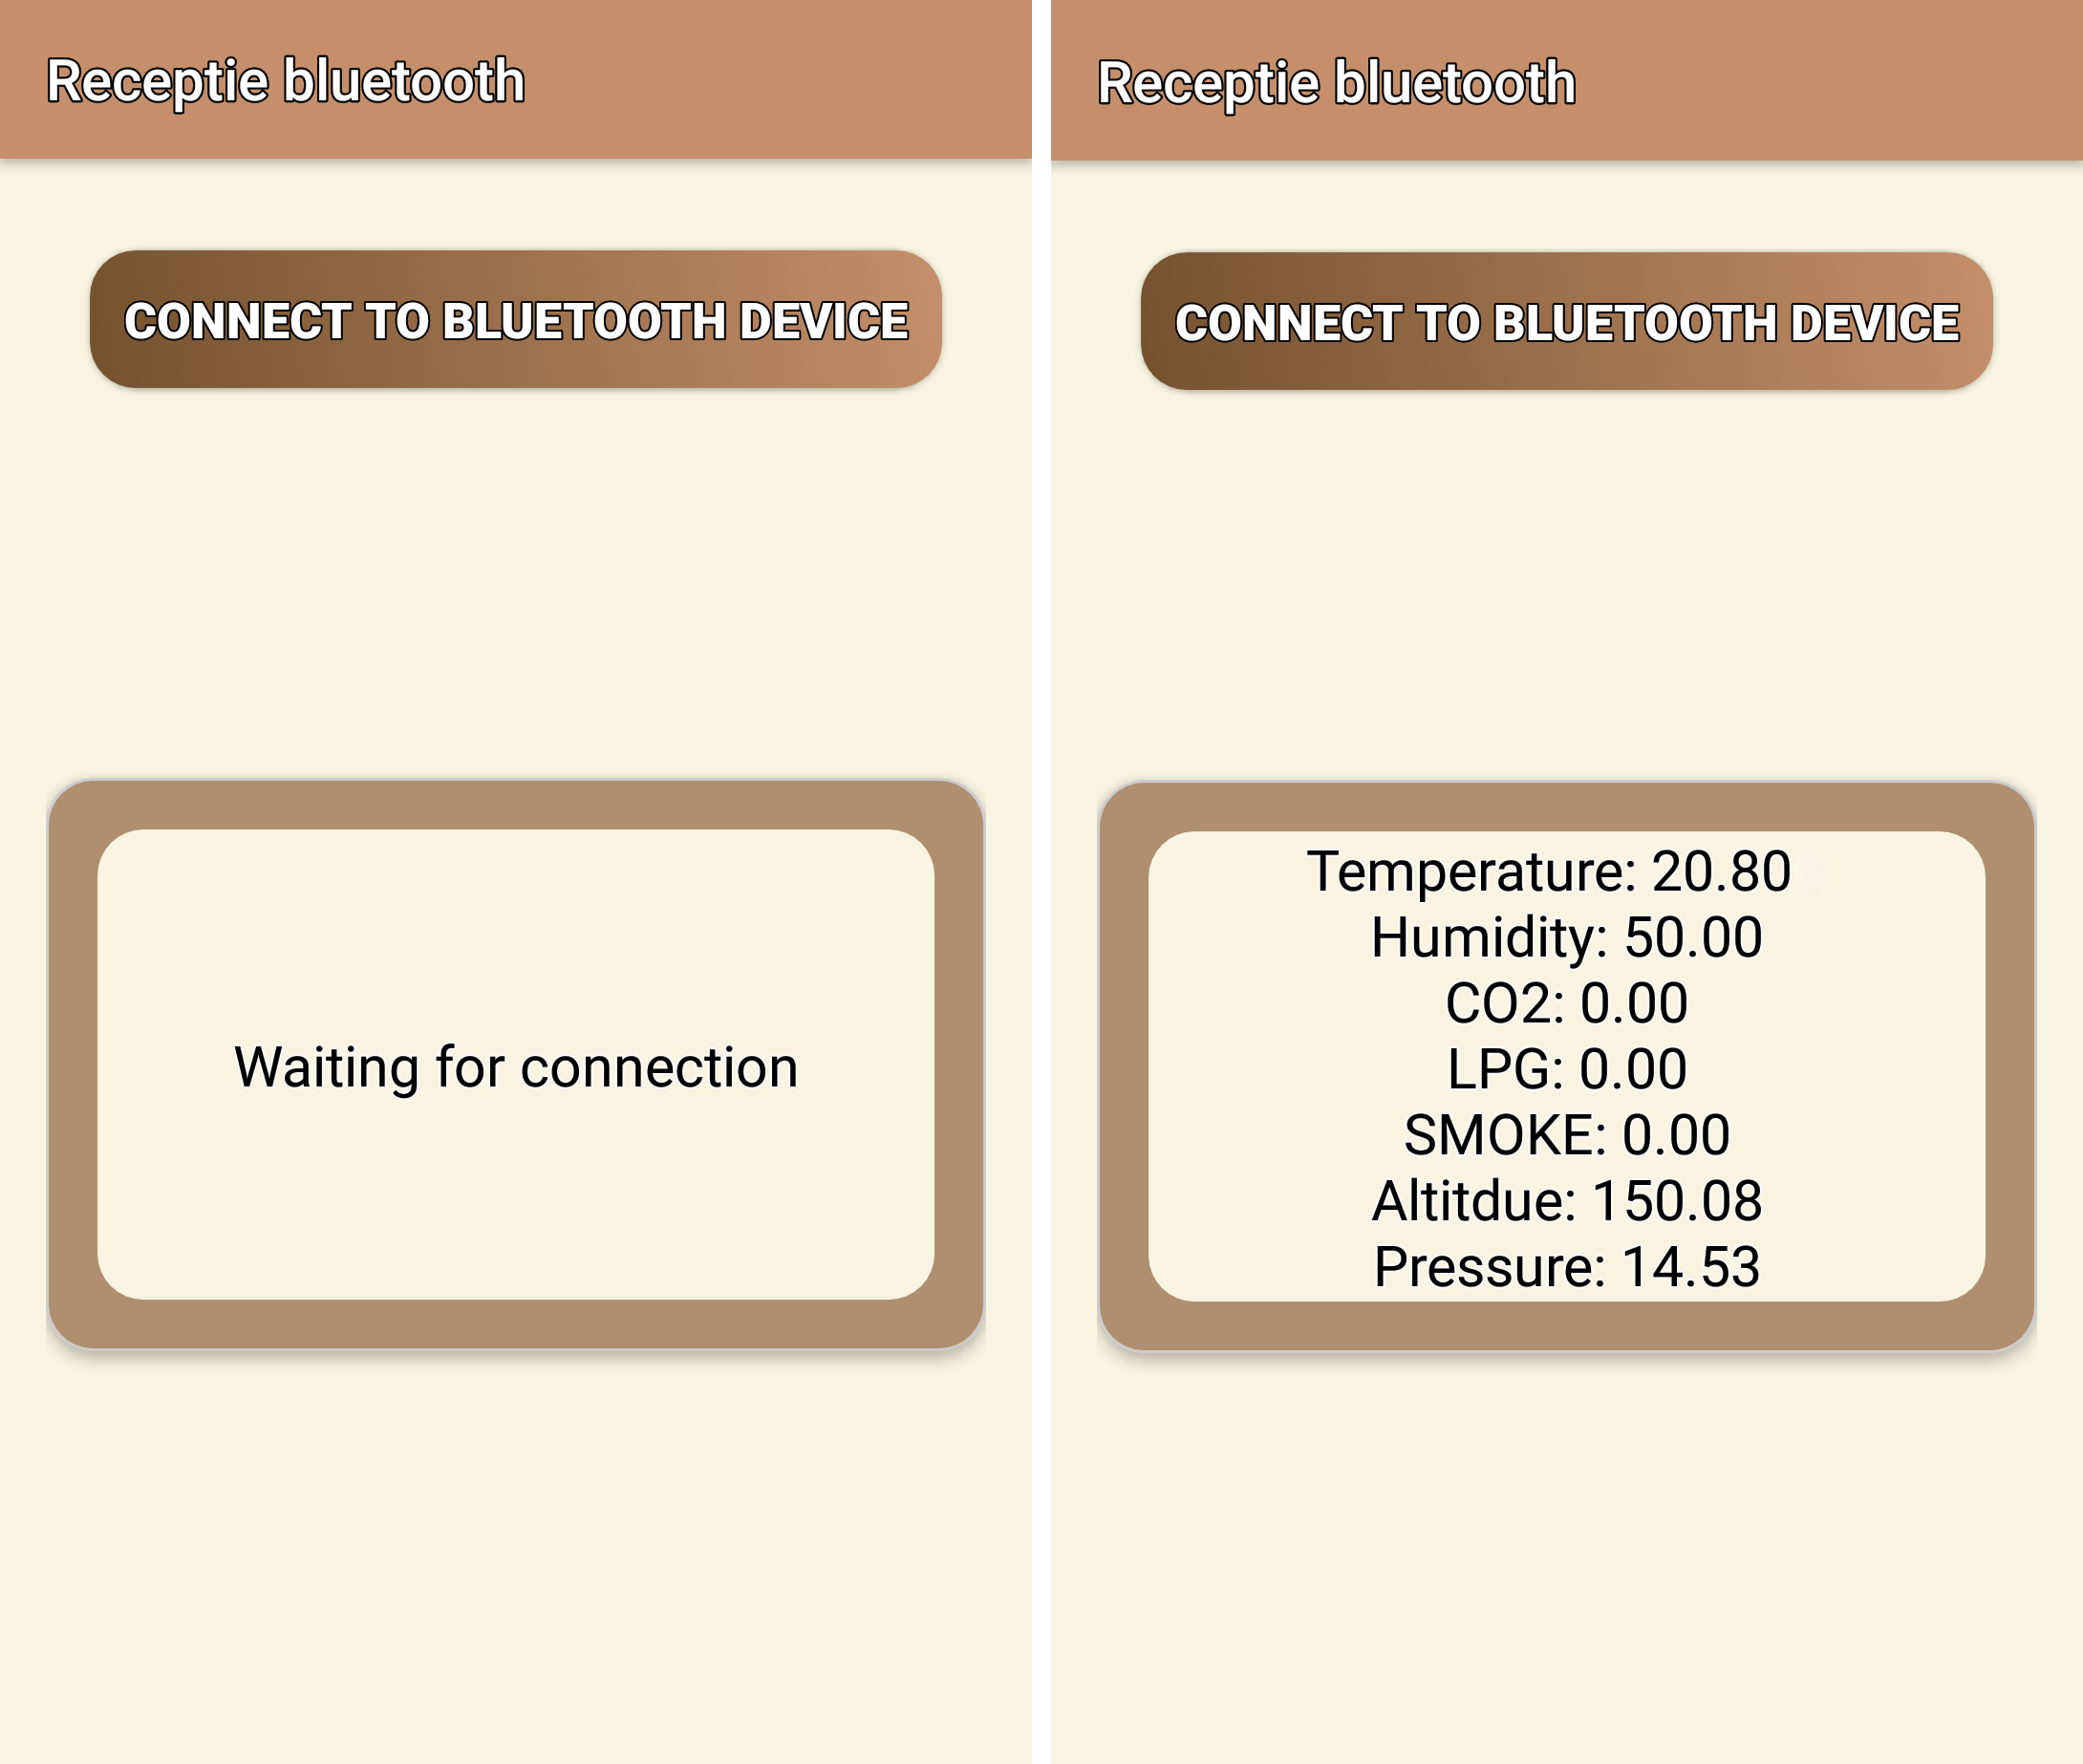
\includegraphics[width=0.6\linewidth]{bachelors_ro/images/bt_app_combined_separted.png}
\caption{Interfața aplicației înainte și după conectare}
\label{fig:bt_app_combined_separted}
\end{figure}

Următorul pas este implementarea codului de conexiune și citire a datelor trimise de modulul Bluetooth. Pentru ca aplicația să poată utiliza Bluetooth-ul este nevoie să ne folosim de API-ul (Application Programming Interface) Bluetooth ofeirt de Android \cite{bt_api}. În Fragmentul \ref{code:bt_api_classes} sunt prezentate clasele ce facilitează conexiunea la Bluetooth a aplicației și adresa MAC (media access control) a modulului. \texttt{deviceUUID} (Universally Unique Identifier) este folosit pentru a identifica tipul de serviciu Bluetooth. String-ul de la linia \textit{(6)} este folosit ca UUID și reprezintă serviciul SPP (Serial Port Profile).

\begin{code}[H]
\begin{lstlisting}[language=Java]
private BluetoothDevice bluetoothDevice;
private BluetoothAdapter bluetoothAdapter;
private BluetoothSocket bluetoothSocket;

private static final String deviceAddress = "**:**:**:**:**:**";
private static final UUID deviceUUID = UUID.fromString("00001101-0000-1000-8000-00805F9B34FB");

\end{lstlisting}
\caption{Clasele folosite din Bluetooth API \cite{bt_api}}
\label{code:bt_api_classes}
\end{code}

Chiar și cu toate datele de conectare oferite în Fragmentul \ref{code:bt_api_classes}, aplicația are nevoie de permisiuni de conectare la BLuetooth ce sunt oferite prin adăugarea Fragmentului \ref{code:bt_permisiuni} în fișierul \texttt{AndroidManifest.xml}.

\begin{code}[H]
\begin{lstlisting}[language=XML]
<uses-permission android:name="android.permission.BLUETOOTH_CONNECT" />
<uses-permission android:name="android.permission.BLUETOOTH"/>
<uses-permission android:name="android.permission.BLUETOOTH_ADMIN"/>
<uses-permission android:name="android.permission.BLUETOOTH_SCAN" />
\end{lstlisting}
\caption{Permisiunile de acces Bluetooth \cite{bt_perm}}
\label{code:bt_permisiuni}
\end{code}

Prima funcție ce trebuie apelată este funcția \texttt{onCreate()} ce inițializează aplicația. În interiorul acesteia avem funcția \texttt{setContentView(R.layout.activity\_main)} ce este apelată cu argumentul \texttt{R.layout.activity\_main} care inițalizează interfața definită anterior. Tot în corupul funcției \texttt{onCreate()} este inițializat și butonul ce conectează telefonul și modulul de Bluetooth. Asupra butonului este executată funcția \texttt{buttonConnect.setOnClickListener} pentru ca în momentul apăsării acesta să realizeze conexiunea cu modulul și să verifice permisiunile de conectare.

\begin{code}[H]
\begin{lstlisting}[language=Java]
private void connectToBluetoothDevice() {
    bluetoothDevice = bluetoothAdapter.getRemoteDevice(deviceAddress);
    try {
         bluetoothSocket = bluetoothDevice.createRfcommSocketToServiceRecord(deviceUUID);
         bluetoothSocket.connect();
        inputStream = bluetoothSocket.getInputStream();
         startReadingData();
    } catch (IOException e) {
        Log.e(TAG, "Error connecting", e);
    }
 }
\end{lstlisting}
\caption{Funcția de conectare la Bluetooth \cite{bt_api}}
\label{code:bt_conexiune}
\end{code}

În Fragmentul \ref{code:bt_conexiune} este prezentată funcția de conectare a dispozitiviului la Bluetooth. Inițial se obține referința către dispozitivul Bluetooth la care dorim să ne conectăm folosind metoda \texttt{bluetoothAdapter.getRemoteDevice(deviceAddress)} în care argumentul reprezintă adresa MAC a dispozitivului. Apoi, la linia \textit{(4)} se creează un socket RFCOMM (Serial Port Profile, iar metoda are ca argument \texttt{deviceUUID} pentru a identifica serviciul de conectare (SPP). După crearea socket-ului, se încearcă conectare cu dispozitivul. Dacă aceasta reușește să se stabilească, se deschide un flux de date, iar funcția \texttt{startReadingData()} este apleată pentru începerea citirii datelor. Dacă conectarea eșuează, se aruncă o excepție.

În Fragmentul \ref{code:bt_read_data} este prezentată metoda \texttt{readData()} ce citește datele primite de la placa de dezvoltare Arduino Mega. Pentru început, este nevoie de un flag \texttt{isReading} pentru a verifica dacă procesul de citire este activ, apoi este declarat obiectul de tip \texttt{Thread} care se ocupă de citirea propriu zisă. La liniile \textit{(4)} și \textit{(5)} avem variabila unde se va stoca șirul de caractere primit (\texttt{buffer}) și indexul acestuia. 

Cu ajutorul buclei \texttt{while(isReading)} menține execuția pornită atât timp cât se pot citi date. Apoi, se încearcă citire unui byte din inputStream, dacă citirea are succes se continuă procesarea datelor. Datele primite au un format special conceput astfel încât un set complet de date are ca terminator simbolul \texttt{\$}. Din acest motiv la linia \textit{(10)} se verifică dacă mesajul a fost transmis în întregime. În cazul în care mesajul este complet, acesta se stochează într-un șir de caractere, indexul buffer-ului se setează pe 0, iar folosind un \texttt{handler} se actualizează câmpul de text pentru a afișa datele primite. \texttt{Thread.sleep(1000)} este folosit pentru a citi datele o dată la o secundă. 


\begin{code}[H]
\begin{lstlisting}[language=Java]
private void readData() {
  isReading = true;
  readThread = new Thread(() -> {
    final byte[] buffer = new byte[1024];
    int bufferPosition = 0;

    while (isReading) {
      try {
        if (inputStream.read(buffer, bufferPosition, 1) > 0) {
          if (buffer[bufferPosition] == '$') {
            final String readMessage = new String(buffer, 0, bufferPosition).trim();
            bufferPosition = 0;
            handler.post(() -> textViewData.setText(readMessage));
            Thread.sleep(1000);
          } else {
            bufferPosition++;
          }
        }
      } catch (IOException | InterruptedException e) {
        Log.e(TAG, "Error reading data", e);
        isReading = false;
      }
    }
  });
  readThread.start();
}
\end{lstlisting}
\caption{Funcția de conectare la Bluetooth \cite{bt_transfer}}
\label{code:bt_read_data}
\end{code}

În final, funcția \texttt{onDestroy()} va asigura închiderea conexiunii și thread-ul de citire este oprit la închiderea aplicației.

Astfel, aplicația a fost creată și poate rula pe orice dispozitiv ce utilizează minim versiunea 6.0 de Android. Rezultatul final este prezent în Figura \ref{fig:bt_app_combined_separted}.


\chapter{Rezultate experimentale}
\thispagestyle{pagestyle}

Un prim experiment efectuat a fost expunerea ansamblului de alarmă la gaze și fum folosind o brichetă. În Figura \ref{fig:chart_gaze} se pot observa fluctuațiile valorilor pentru fum și gaz în intervalul 3:55 - 3:57, timp în care a fost efectuat experimentul. Folosind bricheta, am umplut camera din machetă unde se află senzorul MQ2, răspunsul sistemului fiind cel aștept: atât aplicația mobile, cât și interfața de pe platforma Blynk au arătat aceleași valori crescute, iar alarma a fost declanșată timp de trei secunde pe perioada fiecărei detecții.

\begin{figure}[H]
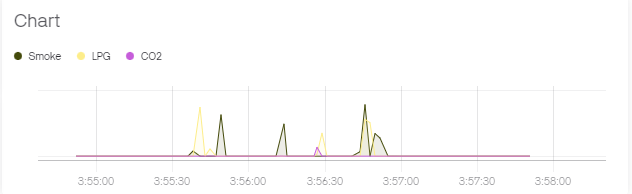
\includegraphics[width=0.8\linewidth]{bachelors_ro/images/chart_gaze.png}
\caption{Nivelul de gaze și fum detectat în urma experimentului}
\label{fig:chart_gaze}
\end{figure}

Un alt experiment efectuat a fost deconectarea sursei ce alimentează ventilatorul și becul pentru a lăsa senzorul să ajungă la temperatura ambientală. Am așteptat până temperatura s-a stabilizat la aproximativ 21 de grade, apoi am reconectat sursa și am setat temperatura dorită la 27 de grade.

\begin{figure}[H]
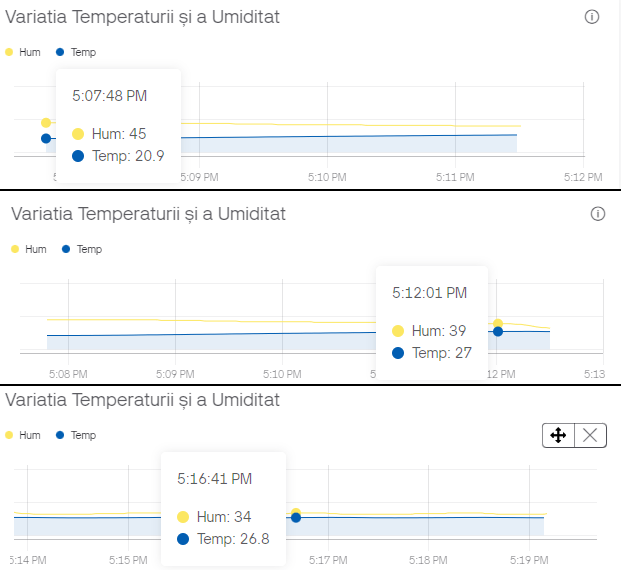
\includegraphics[width=0.5\linewidth]{bachelors_ro/images/combined_chart.png}
\caption{Grafice cu valorile temperaturii în timpul experimentului}
\label{fig:combined_chart}
\end{figure}

Plecând de la 21 de grade Celsius se poate observa în Figura \ref{fig:combined_chart} că termostatul a ajuns la temperatura setată de 27 de grade Celsius în aproximativ 4 minute (intervalul de timp 5:07:48 în primul grafic - 5:12:01 în al doilea grafic). În cel de-al treilea grafic se poate observa stabilitatea sistemului existând variații minore ale temperaturii de +/- 0.5 grade Celsius pe un interval de 5 minute. Concluzionând, ansamblul de stabilizare a temperaturii funcționează corect oferind valori aproape constante, dar și eficient reușind să încălzească 6 grade în doar 4 minute.

\section{Realizarea machetei}

Macheta ce găzduiește sistemul implementat este reprezentată de o casă făcută din plăci de lemn. În Figura \ref{fig:casa_init} se poate observa structura de la care s-a pornit, aceasta fiind un simplu paralelipiped gol. 

\begin{figure}[H]
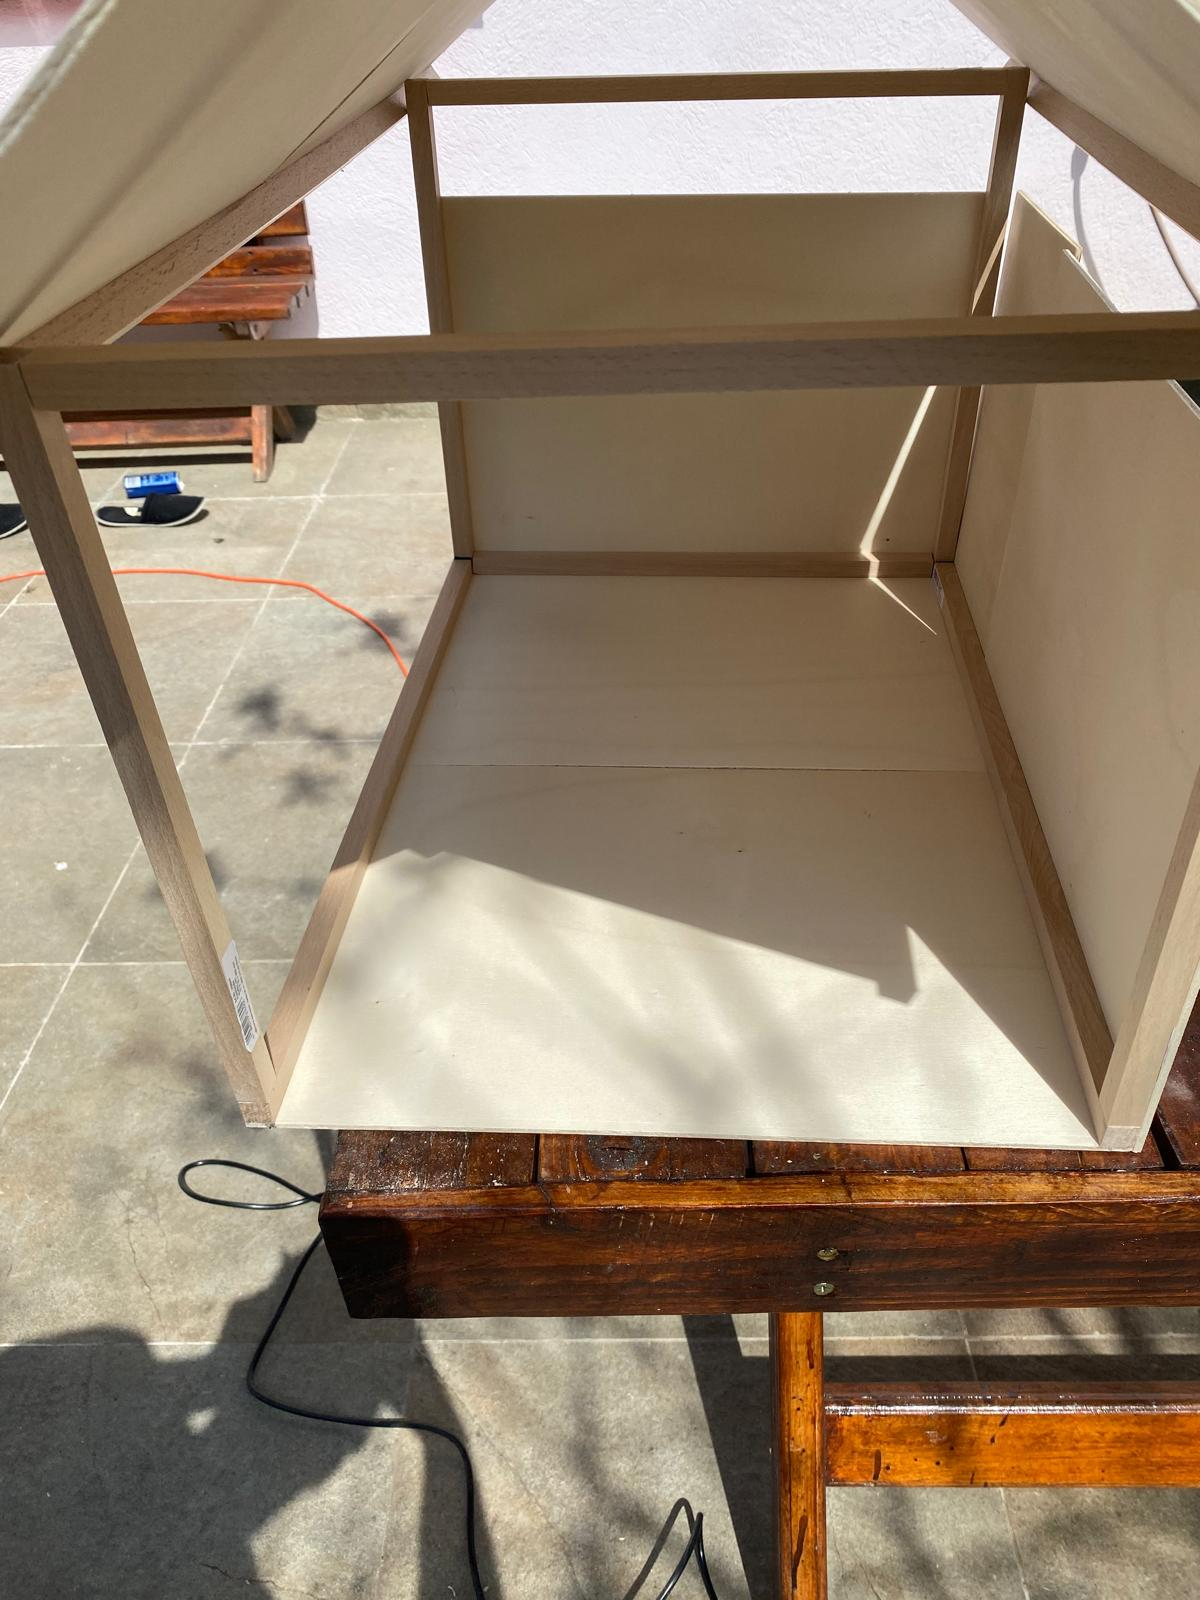
\includegraphics[width=0.3\textwidth, height=0.4\textwidth]{bachelors_ro/images/casa_init.jpg}
\caption{Macheta în stare incipientă}
\label{fig:casa_init}
\end{figure}

În continuare, am decis să construiesc două etaje, la primul etaj să fie folosite 3 camere individuale, una pentru alarma de gaz, una pentru senzorul de mișcare și led-ul controlat aferent și una pentru ușa automată. Astfel, am adăugat pereții necesari și am adăugat o podea pentru al doilea etaj ce reprezintă în același timp și tavanul primului etaj.

În Figura\ref{fig:schema_casa} se poate observa schema casei. Dimensiunile acesteia sunt: L 60 cm x l 42 cm x H 38 cm. Fiecare componentă a fost așezată într-una dintre camere: 1 - senzorul pir și led-ul aferent acestuia, 2 - ansamblul de alarmă, led-ul aferent modului cu fotorezistor și  senzorul BMP280, 3 - ansamblul de stabilizare a temperaturii, 4 - ansamblul de deschidere automată a ușii, 5 - modulul cu fotorezistor.

\begin{figure}[H]
    \centering
    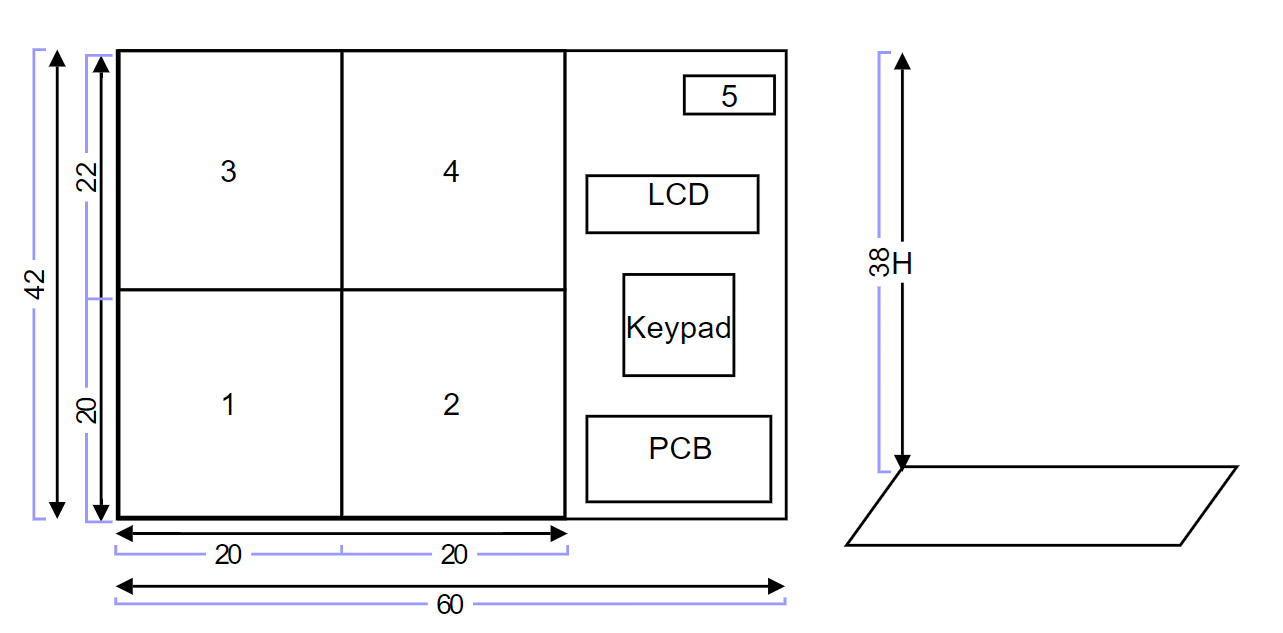
\includegraphics[width=0.8\linewidth]{bachelors_ro/images/schema_casa.png}
    \caption{Schema casei}
    \label{fig:schema_casa}
\end{figure}

Următorul pas după delimitarea arhitecturii a fost decuparea placajului pentru a permite trecerea cablurilor și, unde este cazul, încastrarea componentelor. Ultimul pas a fost să izolez zona ce conține ansamblul de stabilizare a temperaturii în plexiglas. 

În Figurile \ref{fig:casa_din_fata} \ref{fig:casa_de_sus} și \ref{fig:casa_din_lateral} se poate observa rezultatul final al realizării machetei.

\begin{figure}[H]
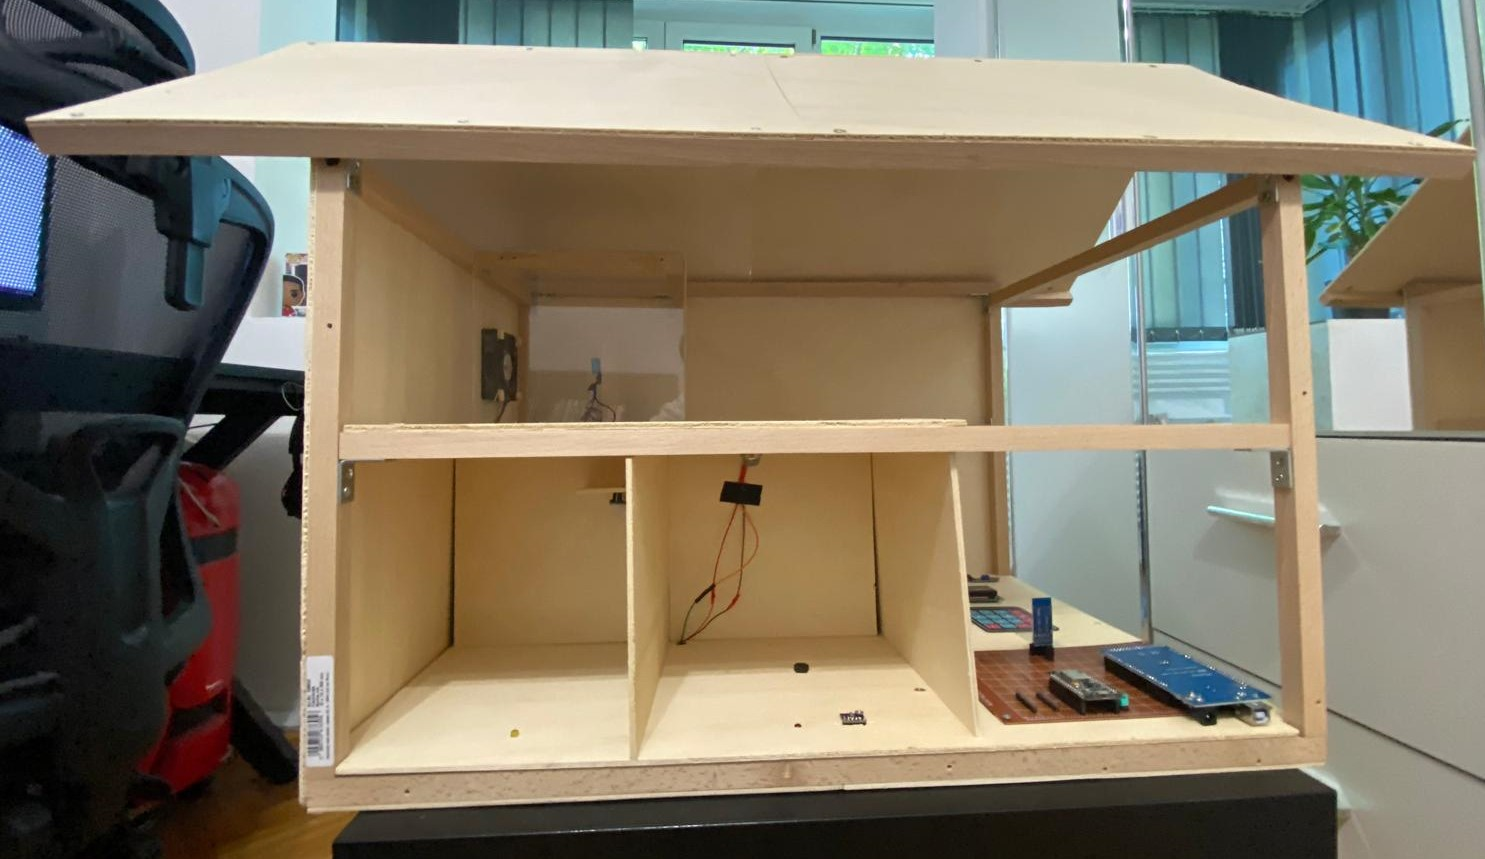
\includegraphics[width=0.6\linewidth]{bachelors_ro/images/casa_din_fata.jpg}
\caption{Macheta văzută din față}
\label{fig:casa_din_fata}
\end{figure}

\begin{figure}[H]
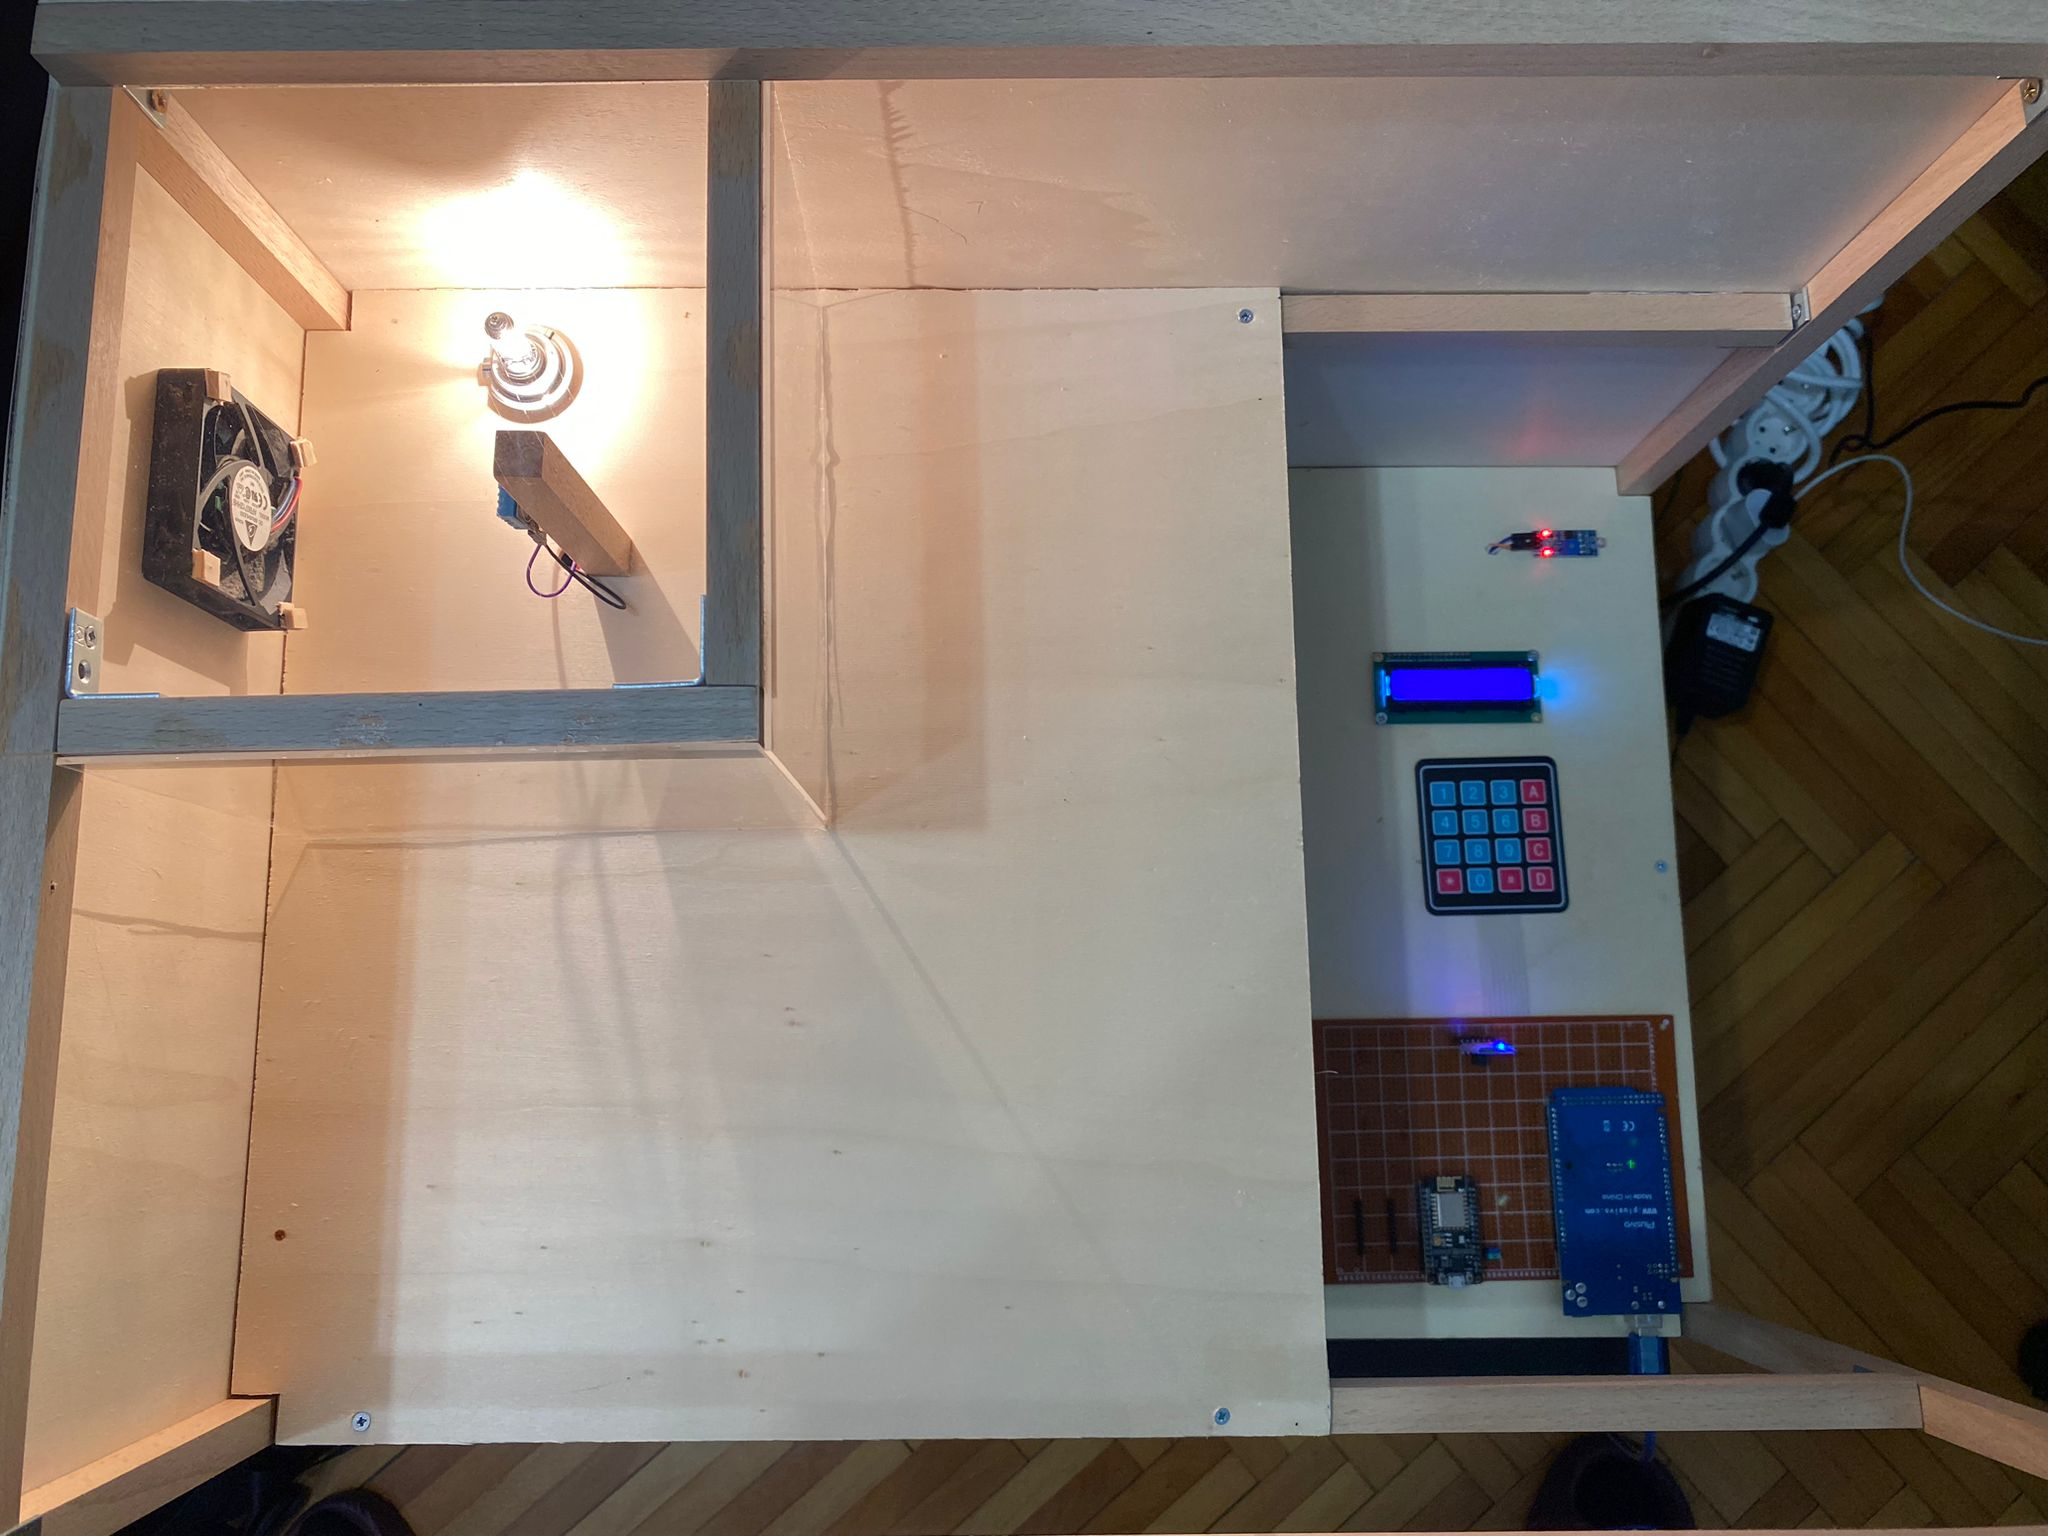
\includegraphics[width=0.6\linewidth]{bachelors_ro/images/casa_de_sus.jpg}
\caption{Macheta văzută de sus}
\label{fig:casa_de_sus}
\end{figure}

\begin{figure}[H]
\includegraphics[width=0.6\linewidth]{bachelors_ro/images/casa_din_lateral.jpg}
\caption{Macheta văzută din lateral}
\label{fig:casa_din_lateral}
\end{figure}

Cablajul a fost realizat inițial la nivel de breadboard (Figura \ref{fig:cablaj_breadboard}. Apoi am realizat că această variantă nu este practică deoarece cablurile se pot deconecta oricând. Astfel am decis să folosesc o placă PCB și să cositoresc toate firele de aceasta creând practic un nucleu al sistemului.

\begin{figure}[H]
\includegraphics[width=0.6\linewidth]{bachelors_ro/images/cablaj_breadboard.jpg}
\caption{Cablaj la nivel de breadboard}
\label{fig:cablaj_breadboard}
\end{figure}

În Figura \ref{fig:cablaj_pcb} se poate observa cablajul montan pe placa PCB. Această placă este încastrată în podeaua machetei. În Figura\ref{fig:pcb_fata} este prezentată placa PCB pe care s-a montat placa de dezvoltare Arduino Mega, modulul NodeMCU și modulul Bluetooth. Macheta dispune de o podea dublă pentru un management al cablurilor facil, acest fapt este prezentat în Figura \ref{fig:podea_dubla}.

\begin{figure}[H]
\includegraphics[angle=90,width=0.7\linewidth]{bachelors_ro/images/cablaj_pcb.jpg}
\caption{Cablaj pe placa PCB}
\label{fig:cablaj_pcb}
\end{figure}

\begin{figure}
    \centering
    \includegraphics[angle=90,width=0.7\linewidth]{bachelors_ro/images/pcb_fata.jpg}
    \caption{Placa PCB văzută de sus}
    \label{fig:pcb_fata}
\end{figure}

\begin{figure}[H]
\includegraphics[width=0.6\textwidth, height=0.4\textwidth]{bachelors_ro/images/podea_dubla.jpg}
\caption{Spatele podelei duble }
\label{fig:podea_dubla}
\end{figure}

\section{Interfețe finale pentru platforma Blynk și aplicația Android}

În Figura \ref{fig:interfata_android} este prezentată interfața finală a aplicației mobile Android dedicată sistemului. Se poate observa butonul de conectare la modulul de Bluetooth și câmpul de date unde sunt afișați parametrii oferiți de senzori.

\begin{figure}[H]
\includegraphics[width=0.6\linewidth]{bachelors_ro/images/bt_app_combined_separted.png}
\caption{Interfața aplicației mobile}
\label{fig:interfata_android}
\end{figure}

Interfețele finale web și mobile, pentru platforma Blynk, sunt prezentate în Figurile \ref{fig:interfata_blynk_web}, respectiv \ref{fig:interfata_blynk_mobile_full}.

\begin{figure}[H]
\includegraphics[width=1\linewidth]{bachelors_ro/images/interfata_blynk_web.png}
\caption{Interfața web a platformei Blynk}
\label{fig:interfata_blynk_web}
\end{figure}

\begin{figure}[H]
\includegraphics[width=0.3\linewidth]{bachelors_ro/images/interfata_blynk_mobile_full.jpg}
\caption{Interfața mobile a platformei Blynk}
\label{fig:interfata_blynk_mobile_full}
\end{figure}

\section{Probleme întâmpinate}

Inițial, pentru proiectul pe care urma să îl implementez, am decis să folosesc Arduino Uno, dar pe măsură ce avansam cu implementarea componentelor am realizat că placa nu oferă performanțele și tehnologiile de care aveam nevoie. Arduino Uno oferă doar un cuplu de pini pentru comunicarea serială, iar eu aveam nevoie de două. Pentru această problemă am decis să folosesc o bibliotecă de comunicare serială software\cite{software_serial_lib}, dar în scurt timp în urma experimentelor am aflat că aceasta este incompatibilă cu biblioteca necesară folosirii servomotorului\cite{servo_lib}. Acest conflict apare în urma faptului că, atât biblioteca dedicată servomotorului, cât și cea pentru comunicarea serială software împart un ceas intern de lucru oferit de placă.

Un alt impediment întâmpinat a fost numărul redus de pini digitali oferit de Arduino Uno. Această placă oferă doar 14 pini digitali din care majoritatea aveau și funcții suplimentare de care aveam nevoie cum ar fi: cei 6 pini ce dispun de PWM(Pulse Width Modulation), cei 2 pini de comunicare serială (RX, TX), cei 2 pini de comunicare prin intermediul protocolului I2C (SDA, SCL)\cite{uno_pinout}.

Ultima problemă de care m-am lovit a fost faptul că memoria flash de 32 KB oferită de Arduino Uno era aproape utilizată în întregime. Memoria SRAM de 2KB era foarte solicitată în timpul execuției programului, astfel reducea performanțele programului\cite{uno_specs}.
\chapter{Concluzii}
\thispagestyle{pagestyle}

\section{Concluzii și perspective de dezvoltare}
Proiectul implementat de automatizare a casei demonstrează funcționalitatea unui sistem complex format din mai multe subansamble precum subansamblul de: stabilizare a temperaturii, de alarmă de gaze și fum, de deschidere automată a ușii și de iluminat. Acest sistem poate fi monitorizat atât la distanțe medii folosind o aplicație Android ce comunică cu sistemul prin Bluetooth, dar și la distanțe mari, comunicând prin WiFi cu platforma Blynk. Sistemul poate fi monitorizat și local prin intermediul unui afișaj local LCD. Folosind macheta, putem observa un exemplu realist în care ansamblele funcționează simultan. 

Perspectivele de dezvoltare de care dispune proiectul sunt vaste. Se pot adăuga diverși noi senzori în funcție de nevoi și control vocal. Totodată, toate interfețele pot fi îmbunătățite sau chiar este posibil să fie adăugate și unele noi.

\section{Sinteza contribuțiilor}

În acest subcapitol voi prezenta contribuțiile aduse de mine acestui proiect:

\begin{itemize}
    \item Realizarea arhitecturii sistemului
    \item Realizarea schemelor de conectare pentru întreg sistemul, dar și pentru fiecare ansamblu în parte
    \item Realizarea cablajului la nivel de breadboard, apoi la nivel de placă PCB
    \item Realizarea schemelor bloc hardware și software
    \item Implementarea software a sistemului pe placa de dezvoltare Arduino Mega
        \begin{itemize}
            \item Implementarea ansamblului de setare al temperaturii
            \item Implementarea alarmei de gaze și fum
            \item Implementarea ansamblului de deschidere automată a ușii
            \item Implementarea iluminatului automat
            \item Conectarea display-ului LCD și al senzorului BMP280 folosind protocolul I2C
            \item Implementarea comunicării seriale între Arduino Mega, modulul NodeMCU și modulul Bluetooth
        \end{itemize}
    \item Implementarea aplicației mobile Android de monitorizarea a sistemului folosind Bluetooth
    \item Crearea interfeței web și mobile și a device-ului Blynk pentru conectarea pinilor virtuali la modulul NodeMCU
    \item Realizarea machetei pentru demonstrarea funcționalității sistemului
\end{itemize}
% Look for building the .bib file on Overleaf documentation
\printbibliography[heading=bibnumbered]

\includepdf[pages={1}]{declaratie_autenticitate_radu.pdf}

\end{document}